\documentclass[11pt,a4paper]{article}

% =============================================================================
% Provisional descriptive companion -- bidding patterns and regulatory context
% =============================================================================
% Standalone document holding descriptive facts about bidding patterns
% (hour-class, firm-class, technology differences) and the regulatory /
% confounder context that surrounds the MTU15 reforms. Its purpose is to give
% the identification strategy a foundation in EMPIRICAL FACTS rather than
% choices that can be re-litigated when the design is iterated on.
%
% Part A: bidding patterns (hour-class, firm-class, technology).
% Part B: regulatory and confounder context (reforzada, zonal dominance,
% CNMC sanctions).
%
% Content was migrated 2026-05-17 from thesis/paper/provisional.tex sections
% 2--13. The regression / identification content from that file lives in the
% sibling document thesis/provisional/regression_results.tex.

\PassOptionsToPackage{table}{xcolor}
\usepackage{amsmath, amssymb, amsthm, mathtools}
\usepackage{dsfont}
\usepackage{graphicx, booktabs, subcaption, tikz, float}
\graphicspath{{../../figures/thesis/}}
\usepackage{array, makecell, multirow}
\usepackage{xcolor}
\usepackage{longtable}
\usepackage[hidelinks]{hyperref}
\usepackage{geometry}
\geometry{a4paper, margin=2.5cm}
\usepackage{pdflscape}
\usepackage{caption}
\captionsetup{font=small, labelfont=bf}

% Color for seasonality-adjusted values shown alongside raw values in tables.
\definecolor{seasoncol}{rgb}{0.10, 0.35, 0.65}

% \code{...} -- monospace path with line-break-at-/-_-. (no \_ escaping needed)
\usepackage{url}
\urlstyle{tt}
\Urlmuskip=0mu plus 1mu\relax
\def\UrlBreaks{\do\/\do\_\do\-\do\.\do\:\do\,}
\newcommand{\code}[1]{\nolinkurl{#1}}

\title{Provisional: descriptive bidding patterns and regulatory context\\[3pt]\large MTU15 thesis companion}
\author{Pablo Paramio}
\date{\today}

\begin{document}
\maketitle

\noindent\emph{This file collects descriptive facts that any identification design must rest on: how firms bid across hour-classes (critical vs flat), how pivotal and non-pivotal firms differ, how technologies differ, and the regulatory / RT2 / reforzada context in which the reforms operate. Nothing here is an identification claim. The regression outputs from the current reform-window design are collected in a companion sibling document.}
% Sibling file: thesis/provisional/regression_results.tex.


\tableofcontents

\clearpage

% =====================================================================
\section*{Glossary of acronyms}\label{sec:bid_internal:glossary}
% =====================================================================
\addcontentsline{toc}{section}{Glossary of acronyms}

\bigskip
\noindent
\renewcommand{\arraystretch}{1.15}
\begin{tabular}{@{}p{2.0cm} p{13.5cm}@{}}
\toprule
\textbf{Acronym} & \textbf{Meaning} \\
\midrule
CCGT & Combined-cycle gas turbine: flexible, dispatchable thermal generator. \\
DA & Day-ahead market (Mercado Diario), cleared once per day. \\
IDA & Intraday auctions (3 European SIDC sessions post-2024-06-14). \\
MCP & Market clearing price. \\
MTU & Market time unit (MTU60 = hourly bidding; MTU15 = 15-minute bidding). \\
ISP15 & Imbalance Settlement Period at 15 minutes (settlement granularity, started 2024-12-01). \\
REE & Red Eléctrica de España, the Spanish transmission-system operator. \\
OMIE & Operador del Mercado Ibérico de Energía, the wholesale market operator. \\
PDBF & Programa Diario Base de Funcionamiento — first post-DA viable schedule (REE-built). \\
PDBC & Programa Diario Base de Casación — pre-PDBF DA-cleared schedule (OMIE-built). \\
PHF & Programa Horario Final — post-IDA + post-RT viable schedule. \\
RES & Renewable Energy Sources (wind, solar PV, solar thermal, RoR hydro). \\
TR & Tiempo Real — real-time restrictions phase (PO 3.4--3.5), pay-as-bid. \\
Fase I/II & Restricciones técnicas Fase 1 (post-PDBF, pre-IDA) and Fase 2 (post-IDA), pay-as-bid. \\
aFRR & Automatic Frequency Restoration Reserve (Regulación secundaria), PICASSO platform. \\
mFRR & Manual Frequency Restoration Reserve (Regulación terciaria), MARI platform. \\
RR & Replacement Reserves (Reserva de Sustitución), TERRE platform. \\
BSP & Balance Service Provider (firm enrolled to supply balancing energy). \\
EUPHEMIA & Day-ahead pan-European auction algorithm (clears DA market). \\
\bottomrule
\end{tabular}
\renewcommand{\arraystretch}{1.0}

\bigskip
\bigskip

% =====================================================================
\section*{Reform-window timeline}\label{sec:bid_internal:timeline}
% =====================================================================
\addcontentsline{toc}{section}{Reform-window timeline}

\noindent The five reform windows used throughout this document are defined as follows. The ``pre-IDA window'' (pre 2024-06-14) is the baseline regime, never directly compared in the main tables but referenced for context.

\begin{figure}[H]
\centering
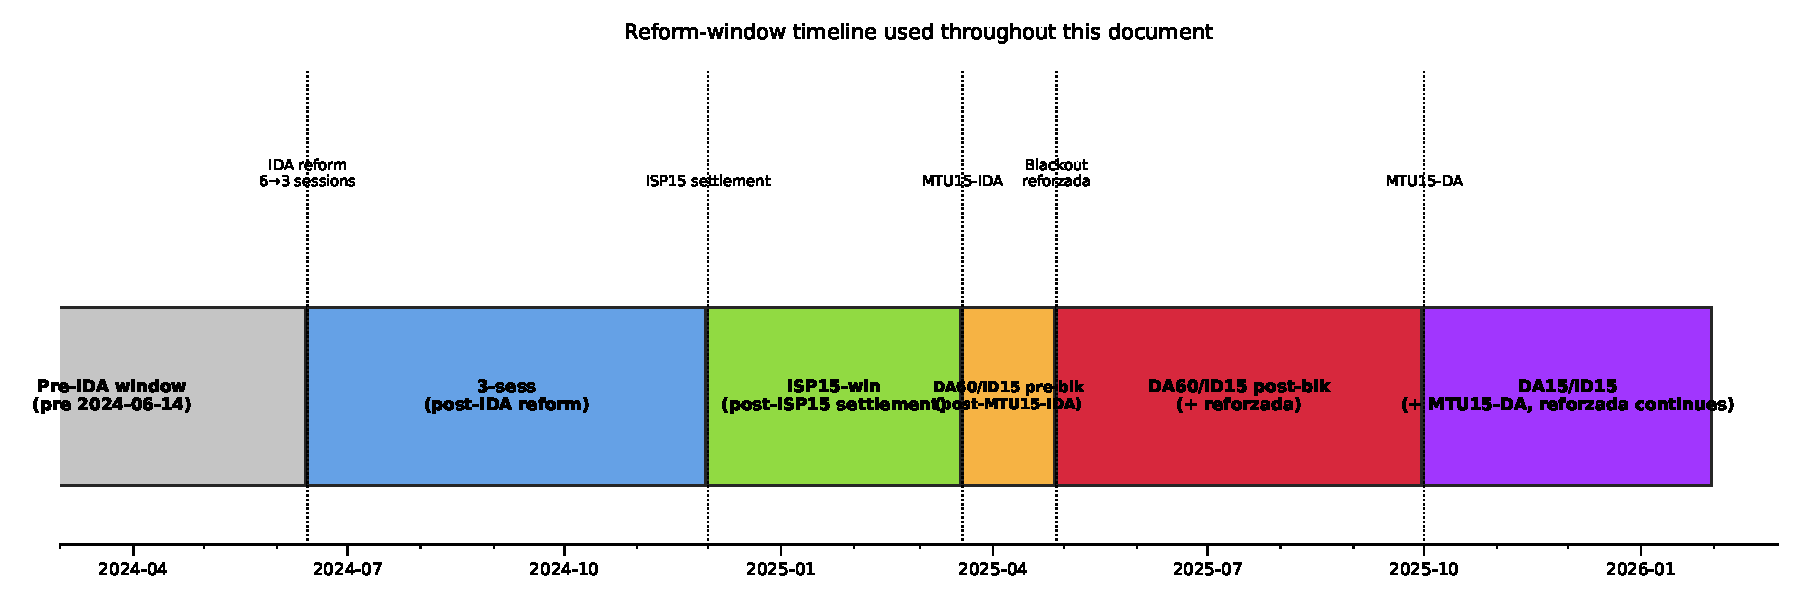
\includegraphics[width=0.98\textwidth]{../../figures/thesis/timeline_reform_windows.pdf}
\caption{\textbf{Reform-window timeline.} Five named windows partition the post-2024-06-14 sample; the pre-IDA window is the baseline regime. Dotted vertical lines mark the five reform dates that produce the window boundaries.}
\label{fig:bid_internal:timeline}
\end{figure}

\bigskip

% =====================================================================
\subsection*{Calendar coverage and same-calendar baselines}\label{sec:bid_internal:calendar_discipline}
% =====================================================================
\addcontentsline{toc}{subsection}{Calendar coverage and same-calendar baselines}

\noindent \textbf{Why this matters.} Spanish electricity is strongly seasonal: heating-driven demand peaks in winter, cooling in summer, hydro inflows peak in spring, solar production peaks at the summer solstice, wind blows hardest in winter. The five reform windows above do \emph{not} span the calendar uniformly --- each window covers a specific subset of calendar months, and these subsets differ across windows. Any cross-regime comparison that does not hold the calendar fixed therefore confounds the regime change with the seasonal pattern. \textbf{This applies to every variable in this document}: bid prices, $D_w$, $\Delta p$ / $\Delta q$, redispatch volumes, imbalance MWh, system-cost levels, RES capture rates. A reader who picks any table in this document should first read Table~\ref{tab:calendar_coverage} below to know which calendar months that regime covers and what comparator is available.

\begin{table}[H]
\centering
\caption{\textbf{Calendar coverage of each reform window, and same-calendar baseline availability.} ``Calendar months covered'' is the set of clock months that fall inside the window. ``Days'' is the window length. ``Same-calendar pre-IDA placebo'' indicates whether a clean same-calendar baseline exists in the pre-IDA period (2018-06-14 through 2024-06-13), where no granularity reform was active. ``Reforzada overlay'' flags windows in which the post-blackout reinforced-operation policy (active 2025-04-28 onward) is also in effect.}
\label{tab:calendar_coverage}
\setlength{\tabcolsep}{4pt}
\scriptsize
\begin{tabular}{@{}>{\raggedright\arraybackslash}p{2.4cm} >{\raggedright\arraybackslash}p{2.6cm} >{\raggedright\arraybackslash}p{2.1cm} r c >{\raggedright\arraybackslash}p{4.4cm}@{}}
\toprule
\textbf{Regime} & \textbf{Calendar dates} & \textbf{Months covered} & \textbf{Days} & \textbf{Reforzada?} & \textbf{Same-calendar pre-IDA placebo} \\
\midrule
\textbf{pre-IDA} & $\le$ 2024-06-13 & all 12, multi-year & -- & no & N/A (is the baseline) \\
\textbf{3-sess} & 2024-06-14 -- 2024-11-30 & Jun--Nov & 170 & no & Clean (Jun--Nov 2018--2023) \\
\textbf{ISP15-win} & 2024-12-01 -- 2025-03-18 & Dec--Mar & 108 & no & Clean (Dec--Mar 2018--2024) \\
\textbf{MTU15-IDA pre-blk} & 2025-03-19 -- 2025-04-27 & late Mar -- Apr & 40 & no & Clean (same 40 days 2018--2024) \\
\textbf{MTU15-IDA post-blk} & 2025-04-28 -- 2025-09-30 & May -- Sep & 156 & \textbf{yes} & Clean for granularity (May--Sep 2018--2023, pre-IDA); none for reforzada (no pre-2025-04-28 reforzada in data) \\
\textbf{DA15/ID15} & 2025-10-01 -- present & Oct--May (partial, ongoing) & 220+ & \textbf{yes} & None clean. 2024--25 same-calendar comparators are themselves a mix of post-MTU15-IDA + ISP15-win regimes \\
\bottomrule
\end{tabular}
\end{table}

\noindent\textbf{Three categories.} Each regime falls into one of three buckets for the purpose of cross-regime reading:

\begin{enumerate}\setlength{\itemsep}{2pt}
\item \textbf{Clean same-calendar placebo available.} \emph{3-sess, ISP15-win, MTU15-IDA pre-blk.} For each of these, we can restrict the pre-IDA baseline to the same calendar months in 2018--2024 (and average across years), and the difference (regime $-$ pre-IDA same-cal) is interpretable as the regime effect with seasonality differenced out. Any cross-regime reading that uses these windows defaults to this same-calendar comparison unless explicitly stated otherwise.

\item \textbf{Reforzada-confounded, partial calendar-match available.} \emph{MTU15-IDA post-blk.} The window spans May--Sep 2025, which has clean same-calendar comparators in pre-IDA (May--Sep 2018--2023). But these comparators are pre-reforzada. So the difference (MTU15-IDA post-blk $-$ pre-IDA same-cal) confounds (a) the granularity reform, (b) operación reforzada, and (c) the post-blackout system state. There is no calendar period in the data in which reforzada is active but MTU15 is not, so reforzada cannot be differenced out via a same-calendar pre-reform window. For descriptive purposes, May--Sep 2025 is best read as ``post-MTU15-IDA $+$ reforzada $+$ post-blackout, jointly''; see \S\ref{sec:prov:phf_minus_pdbf} on disentangling these channels.

\item \textbf{No clean calendar match.} \emph{DA15/ID15.} The window covers Oct 2025 onward. The same calendar months one year earlier (Oct 2024 -- May 2025) are themselves a mix of pre-MTU15-IDA, ISP15-win, MTU15-IDA pre-blk, and MTU15-IDA post-blk regimes --- so calendar-matching to ``one year ago'' does not produce a single-regime comparator. The cleanest available calendar comparators for DA15/ID15 are the same months in pre-IDA years (Oct 2023 -- May 2024 was largely pre-IDA, with the IDA-3 reform starting only mid-Jun 2024; Oct 2022 -- May 2023 and earlier are all pre-IDA). But even with pre-IDA same-calendar baselines, the reforzada overlay is unresolved by this comparator: DA15/ID15 is the union of MTU15-DA, MTU15-IDA, and reforzada in the same calendar window, and our data does not contain a period where any one of these three is active without the others. Therefore any DA15/ID15 reading should be flagged as descriptive only, with the three confounds explicitly named.
\end{enumerate}

\noindent\textbf{Fourier-deseasonalization.} For a daily outcome $y_t$ we fit a pooled Frisch-Waugh-Lovell regression on $t \in [2022\text{-}01\text{-}01, 2026\text{-}05\text{-}15]$:
\[
g(y_t) \;=\; \alpha \;+\; \sum_{r} \beta_r \,\mathbf{1}\{\text{regime}(t) = r\} \;+\; \sum_{k=1}^{4} \left[ a_k\, c_k(t) + b_k\, s_k(t) \right] \;+\; \sum_{j=1}^{6} \delta_j\, \mathbf{1}\{\operatorname{dow}(t) = j\} \;+\; \varepsilon_t,
\]
with omitted regime pre-IDA, link $g$ equal to $\log$ for positive levels and $\operatorname{logit}$ for bounded shares, and day-of-year sinusoids $c_k(t)=\cos(2\pi k\,\operatorname{doy}(t)/365)$, $s_k(t)=\sin(2\pi k\,\operatorname{doy}(t)/365)$. Four harmonics (annual, semi-annual, four-month, quarterly) capture the seasonal cycle; the six day-of-week dummies absorb weekly periodicity. Seasonality is pooled across regimes because the 40-day MTU15-IDA pre-blk window cannot identify regime-specific Fourier coefficients.

\paragraph{Seasonality-adjusted (SA) value.} $\hat y_r^{\text{SA}}$ is the predicted level of $y$ in regime $r$ at annual-mean Fourier (zero by orthogonality) and within-week DOW mean, with a Duan-smearing correction across in-sample residuals $\{\widehat e_i\}$ for the non-linear link:
\[
\hat y_r^{\text{SA}} \;=\; \frac{1}{n}\sum_{i=1}^{n} g^{-1}\!\left(\widehat\alpha + \widehat\beta_r + \tfrac{1}{7}\sum_{j=1}^{6}\widehat\delta_j + \widehat e_i\right).
\]
In tables, SA values sit in {\color{seasoncol}coloured brackets} next to the raw regime mean (omitted where the value is calendar-matched by construction). Where raw and SA move the same way the pattern survives seasonality control; where they diverge, only the SA value is comparable across regimes. For the reforzada-confounded windows (MTU15-IDA post-blk, DA15/ID15) the SA value still bundles granularity, reforzada, and the post-blackout system state --- it differences out the calendar, not the policy overlap.

\bigskip

\noindent\textbf{Reading guide.} Part A is about bidding and trading patterns. Part B is about the regulatory/post-clearing channels (reforzada, geographic dominance, CNMC sanctions, etc.) that are independent of the granularity reform but constrain how the identification can be set up.

% =============================================================================
\part{Synthesis --- read this first}\label{sec:prov:synthesis}
% =============================================================================

\noindent\emph{Executive summary: the phenomenon, the mechanism, and what each reform did, written for a reader who has not yet seen Parts~A and~B. Every claim points to the figure or table in those parts that sustains it. Numbers tagged {\color{seasoncol}(SA)} are seasonally adjusted; (cal-matched) are same-calendar-month comparisons; untagged numbers are raw.}

\section{The setting}\label{sec:prov:synthesis:setting}

\begin{itemize}\setlength{\itemsep}{3pt}
\item \textbf{Four market reforms in sixteen months}: intraday auctions $6 \to 3$ European sessions (Jun 2024); 15-min imbalance settlement (ISP15, Dec 2024); 15-min intraday auctions (MTU15-IDA, Mar 2025); 15-min day-ahead (MTU15-DA, Oct 2025). Calendar map: Table~\ref{tab:calendar_coverage}.
\item \textbf{Cutting across them}: the 28~April 2025 Iberian blackout and the \emph{operación reforzada} stance that followed --- the system operator keeps voltage-fragile-zone gas plants physically running whether or not they cleared the market.
\item \textbf{The intuition for the whole document}: the reforms are a \emph{granularity} story, reforzada is a \emph{market-power} story; they overlap in calendar time, and everything here is about telling the two apart.
\end{itemize}

\section{The headline phenomenon: combined-cycle gas leaves the auction}\label{sec:prov:synthesis:phenomenon}

\begin{itemize}\setlength{\itemsep}{3pt}
\item \textbf{The four big combined-cycle gas (CCGT) operators stopped clearing the day-ahead market.} DA-cleared volume fell $83\%$ same-calendar-month, Dec 2024 $\to$ Dec 2025 ($1{,}444 \to 244$ GWh, Table~\ref{tab:q1_drop_by_tech}); every other technology held flat or grew.
\item \textbf{The intuition: the gas did not stop generating --- it stopped generating \emph{through the auction}.} The output reappears on a different channel.
\item The ``post-DA gap'' (final program minus day-ahead-plus-bilateral) rose $\sim +1{,}044$ GWh/month for CCGT after the blackout, and \emph{fell} for every other technology on the same channel (Table~\ref{tab:gap_pretrends}).
\item Deseasonalised, the CCGT post-DA gap goes $\sim 47$ GWh/day (3-sess baseline) $\to \sim 389$ GWh/day (post-blackout) {\color{seasoncol}(SA)} --- a structural break, not a seasonal wobble. The gas plants increasingly get dispatched by the operator \emph{after} the auction clears, rather than competing inside it.
\end{itemize}

\section{The mechanism: stay out, get recalled, get paid more}\label{sec:prov:synthesis:mechanism}

\noindent\emph{Why would a profit-maximising plant walk away from the market it exists to sell into? Because being recalled afterwards pays better.} Four observable steps:

\begin{itemize}\setlength{\itemsep}{3pt}
\item \textbf{Stay out.} Naturgy's CCGT fleet bids $\sim\texteuro 840$/MWh in every zone --- dominant or not, 2024 and 2025 (cal-matched, Table~\ref{tab:bid_by_zonal_dominance}). Far above any plausible clearing price: a bid engineered \emph{not} to clear.
\item \textbf{Get recalled.} The operator adds the plant back via post-clearing redispatch under reinforced-operation security criteria. That leg --- ``Fase~I'' --- is paid \emph{pay-as-bid}, not at a uniform market price (\S\ref{sec:prov:phf_minus_pdbf}): a locally-indispensable plant names its own price on the recall.
\item \textbf{Collect the markup.} Fase~I-up averaged $\texteuro 168$/MWh under DA15/ID15 vs a bottom-up CCGT marginal cost of $\texteuro 100$--$110$ --- a $30$--$60\%$ markup over cost. And it \emph{widened} across the reform sequence: $\texteuro 44$--$59$/MWh premium at 3-sess $\to \texteuro 58$--$68$ at DA15/ID15 (Table~\ref{tab:mc_ccgt_premium}).
\item \textbf{Concentrated, and not new.} Naturgy alone captures $\sim$half of Big-4 post-clearing CCGT revenue (Table~\ref{tab:ccgt_post_clearing_rev}); per-day take $\sim\texteuro 2$M pre-reforzada $\to \sim\texteuro 5$--$8$M post. The CNMC sanctioned Naturgy for exactly this practice, same southern-corridor plants, in 2016--2017 (Table~\ref{tab:cnmc_sanctions}, expediente SNC-DE-175-17). \emph{The reforms did not invent the strategy --- they changed which channel makes it pay.}
\end{itemize}

\section{What each reform actually did}\label{sec:prov:synthesis:per_reform}

\begin{itemize}\setlength{\itemsep}{3pt}
\item \textbf{ISP15 (settlement, Dec 2024) --- the cleanest to read}, nothing else changed in its window. 15-min imbalance settlement mechanically shrinks the within-hour variance that gets settled: imbalance volume per cell fell $\sim 60\%$ --- $\sim 50$ pp mechanical variance-averaging $+\sim 10$ pp genuine behavioural improvement in balance-responsible-party forecasting (\S\ref{sec:prov:full_cascade:efficiency}).
\item \textbf{MTU15-IDA (intraday, Mar 2025) --- the biggest genuine efficiency gain.} 15-min intraday products mean within-hour scarcity gets resolved \emph{in the auction} instead of bleeding into real-time emergency redispatch. Real-time technical-restriction cost: $\sim\texteuro 5.8$M/day $\to \sim\texteuro 2.9$M/day $\to \sim\texteuro 1.2$M/day {\color{seasoncol}(SA)} by DA15/ID15 (Table~\ref{tab:efficiency_gains}, Fig.~\ref{fig:efficiency_gains}).
\item \textbf{MTU15-DA (day-ahead, Oct 2025) --- the hardest to read}, its window sits entirely inside reforzada. Small extra efficiency ($\sim\texteuro 1.5$M/day real-time + reserve savings) but the window also carries reforzada-driven Fase~I cost growth ($+\texteuro 2.5$M/day). Net per-day adjustment cost \emph{rises} --- not because granularity failed, but because the reinforced-operation stance is expensive and shares the calendar window. Fig.~\ref{fig:efficiency_gains} shows it: MTU15 channels shrink bar by bar while the Fase~I channel grows. The two are logically distinct; we never report their sum as ``the effect of MTU15-DA''.
\end{itemize}

\section{Who responds, and how their bidding changes}\label{sec:prov:synthesis:het}

\begin{itemize}\setlength{\itemsep}{3pt}
\item \textbf{The strategic actor is combined-cycle gas}; granularity handed it a new margin. Before MTU15, one price-quantity schedule per clock-hour; after, four within-hour schedules it can shape differently.
\item We measure that shaping two ways (\S\ref{sec:prov:dw_tables}): \emph{per-curve} metrics --- the price spread $\sigma_p$ and effective tranche count $N_{\text{eff}}$ of each single bid curve --- and the \emph{pairwise} $D_w$ dissimilarity between a unit's four within-hour quarter curves near MCP. For CCGT in critical hours, the share of cells with non-trivial within-hour shaping ($D_w > 0$) roughly \emph{doubles} across the three MTU15-IDA regimes (Table~\ref{tab:ida_pre_post}); hydro and pumped hydro move the same direction, weaker. \emph{The granular market created a new pricing margin, and the technologies with market power in the high-stakes hours exercised it.}
\item \textbf{No longer a one-firm story}: under DA15/ID15 all four big CCGT firms shape their within-hour bids (HC $79\%$, GE $75\%$, GN $72\%$, IB $59\%$ of critical-hour cells); before the blackout it was concentrated at Naturgy.
\item \textbf{Caveat for the regression design}: the critical-versus-flat asymmetry --- the backbone of the identification --- still holds in direction (CCGT $71\%$ critical vs $51\%$ flat under DA15/ID15) but is now a matter of \emph{degree}, not a clean treated-versus-untreated split: flat hours are no longer ``unshaped''.
\end{itemize}

\section{What this means for identification}\label{sec:prov:synthesis:scope}

\begin{itemize}\setlength{\itemsep}{3pt}
\item The three granularity reforms overlap in time with reforzada; the MTU15-DA window sits \emph{entirely} inside it. No single regression can be read as ``the effect of MTU15-DA'' without conflating a genuine granularity efficiency with a reforzada-driven cost.
\item \textbf{Strategy} (companion document \code{regression\_results.tex}): choose reform windows in which reforzada is held constant, and read each outcome one at a time rather than as one bundled effect.
\item \textbf{External check the mechanism is real} (not a measurement artefact): the CNMC's 2019 sanction (SNC-DE-175-17) and its 2026 expediente cohort pursue precisely the stay-out-and-get-recalled conduct documented here.
\end{itemize}

\bigskip
\noindent The rest of the document is the evidence base. Part~A documents the bidding and trading patterns one technology, one firm, one hour-class at a time; Part~B characterises the regulatory and post-clearing channels (reforzada, geographic dominance, CNMC enforcement) that surround the granularity reforms and constrain how the identification can be set up.

% =============================================================================
\part{Part A --- Bidding and trading patterns}
% =============================================================================

\noindent\emph{Reading guide for Part A.} Three setup sections come first. \S\ref{sec:prov:hour_class} defines the \textbf{hour-class taxonomy} (critical / flat / midday) used to slice every table and figure that follows. \S\ref{sec:prov:pricesetter} characterises \textbf{who price-sets} in the day-ahead market (\S\ref{sec:prov:pricesetter_da}) and, methodologically, in the intraday markets (\S\ref{sec:prov:pricesetter_ida}). \S\ref{sec:prov:dw_decomp} then defines the \textbf{bid-shape metrics} in two families: \emph{per-curve functionals} (one scalar per single bid curve --- $\sigma_p$, $N_{\text{eff}}$, the fPCA scores) and \emph{pairwise divergences} (a statistic of two curves --- $D_w$, $\Delta p$, $\Delta q$). Visual results (per tech $\times$ firm $\times$ quarter bid curves with mean clearing prices overlaid) come in \S\ref{sec:prov:bid_graphs}; quantitative tables come in \S\ref{sec:prov:dw_tables}.

% =====================================================================
\section{Hour-class taxonomy: critical, flat, midday}\label{sec:prov:hour_class}
% =====================================================================

\paragraph{Empirical classification: within-hour standard deviation of residual demand.}
The crit/flat/midday split is \textbf{not assumed} on demand-level grounds (``critical hours are the ones with the highest demand''). It is derived from the within-hour \emph{variability} of residual demand. The intuition is mechanical: \emph{MTU15 granularity has economic content only where the within-hour profile actually moves}. If residual demand is essentially flat within a clock-hour, the hourly clearing price is already a good summary; granular per-quarter pricing has no signal to add. If residual demand changes sharply within the hour (morning ramp, evening peak, solar fade), the hourly clearing price was a compromise across rapidly-changing within-hour conditions; granular pricing unlocks the ability to discriminate across quarters and is therefore where strategic bidding can have a quarter-specific footprint.

Concretely, for clock-hour $h$ on date $d$, let $D_{h,q,d}$ be the residual demand (= load $-$ wind $-$ solar) at quarter $q \in \{1,2,3,4\}$ of that hour. The hour's quarter-mean is $\bar D_{h,d} = \tfrac{1}{4}\sum_q D_{h,q,d}$. We compute, per (date, hour), the within-hour standard deviation
\[
 \sigma_{\text{within}}(h, d) \;=\; \sqrt{\tfrac{1}{4}\sum_{q=1}^{4}\bigl(D_{h,q,d} - \bar D_{h,d}\bigr)^2},
\]
and take the expectation over all 2025 dates to get a clock-hour metric
\[
 \sigma_{\text{within}}(h) \;=\; \mathbb{E}_d\bigl[\sigma_{\text{within}}(h, d)\bigr] \quad [\text{MW}].
\]
The 24-hour ranking of $\sigma_{\text{within}}(h)$ is the actual driver of the classification. Hours with high $\sigma_{\text{within}}$ are critical; hours with low $\sigma_{\text{within}}$ are flat; midday hours are excluded for a separate reason (below). In economic terms, high $\sigma_{\text{within}}$ means the within-hour residual-demand curve moves enough that equilibrium quarter prices and quantities should differ; hour-level pricing was a binding pooling constraint, and granular pricing relaxes it. Strategic firms with within-hour market power therefore have scope to exploit it in critical hours and essentially no scope in flat hours --- which is the heterogeneity Part A's CCGT bid-shape analysis is set up to detect.

\paragraph{Data, window, and frequency.}
$D_{h,q,d}$ is computed from two ENTSO-E Transparency Platform sources, both at 15-minute ISP resolution:
\begin{itemize}
\item Spanish system load: ENTSO-E A65 (ENTSO-E A65 load series), filtered to MTU = 15 minutes.
\item Spanish wind + solar generation: ENTSO-E A75 (ENTSO-E A75 wind+solar actual generation series), PSR types B16 (solar) + B18 (wind offshore) + B19 (wind onshore), filtered to MTU = 15 minutes.
\end{itemize}
Residual demand is the per-ISP arithmetic difference $D = \text{load} - \text{solar} - \text{wind}$.

\emph{Window.} The classifier runs on 2023-01-01 through 2026-05-14 ($\approx 3.4$ years), the largest window for which both A65 and A75 are uniformly available at 15-min granularity (pre-2023 the series are 60-min, so within-hour variance is undefined). The classifier is a structural feature of the within-day pattern, not a regime-specific statistic; all dates are pooled (weekday + weekend) and the weekday-only partition produces the same class assignments.

\paragraph{The 24-hour ranking.}
Table~\ref{tab:hour_classification_full} is reproduced from the main paper's Appendix~A.7. It shows the per-hour mean load, solar, wind, residual demand, $\sigma_{\text{within}}$, the coefficient of variation $\text{CV} = \sigma_{\text{within}} / \overline{\text{residual demand}}$, and the signed within-hour load change $\Delta\text{load} = \text{load}_{q_4} - \text{load}_{q_1}$, averaged over all dates 2023-01-01 through 2026-05-14. The critical-flat-midday classification falls out of $\sigma_{\text{within}}$ directly.

\emph{Why the CV column.} Both the \emph{absolute} within-hour swing ($\sigma_{\text{within}}$) and the \emph{level} of residual demand it sits on matter, and they need not rank hours the same way. The CV --- the swing normalised by the level --- makes the difference visible. Two readings stand out. First, the evening-peak hours 19h--22h are critical on $\sigma_{\text{within}}$ ($522$--$781$ MW) but have a \emph{low} CV ($2.3$--$3.9\%$), because residual demand is at its daily maximum ($\sim 20$--$23$ GW) and divides the swing down --- their within-hour curve moves a lot in MW but little relative to its own height. Second, the morning-ramp and evening-transition hours (08h, 16h) carry the highest CV ($7.5$--$9.0\%$): a large swing on a comparatively thin residual-demand base, the configuration in which a within-hour price-setter has the most relative room to discriminate. The classifier remains $\sigma_{\text{within}}$ --- the CV is shown as complementary context, not as an alternative threshold --- but the CV column flags that ``critical'' is not a uniform category: the morning ramp and the evening peak are critical for different reasons.

\begin{table}[H]
\centering\footnotesize
\caption{\textbf{Hour-of-day classification metrics, Spain 2023--2026} (ENTSO-E A65 + A75, 15-min ISP, $n \approx 3.4$ years of daily observations per hour). The classifier is $\sigma_{\text{within}}$ (column 6, MW). Critical hours: $\sigma_{\text{within}} \in [522, 1303]$. Flat hours: $\sigma_{\text{within}} \in [336, 357]$. Midday: $\sigma_{\text{within}} \in [468, 502]$ --- intermediate, but excluded for the separate reason discussed below. Dropped (transition) hours sit at the regime boundaries. \textit{Year-stability:} across the 3 full years 2023, 2024, 2025 (computed separately), the critical-set min $\sigma_{\text{within}}$ across years is 530 MW, exceeding the flat-set max (387 MW) by $1.4\times$; no within-class swaps across years.}
\label{tab:hour_classification_full}
\newcommand{\critrow}{\rowcolor{red!10}}%
\newcommand{\flatrow}{\rowcolor{blue!10}}%
\begin{tabular}{r r r r r r l}
\toprule
$h$ & load (GW) & solar (GW) & net-load (GW) & $\sigma_{\text{within}}$ (MW) & $\Delta$load (MW) & class \\
\midrule
{ 0} & 23.2 & 0.2 & 16.1 & 398 & -864 & \textit{dropped} \\
\textit{ 1} & 22.4 & 0.1 & 15.4 & 356 & -481 & \textit{flat} \\
\textit{ 2} & 22.0 & 0.1 & 15.1 & 272 & -193 & \textit{flat} \\
\textit{ 3} & 21.9 & 0.1 & 15.2 & 328 & +194 & \textit{flat} \\
{ 4} & 22.9 & 0.1 & 16.3 & 654 & +1179 & \textit{dropped} \\
\textbf{ 5} & 24.9 & 0.3 & 18.4 & 768 & +1795 & \textit{critical} \\
\textbf{ 6} & 27.0 & 1.9 & 18.9 & 1004 & +1420 & \textit{critical} \\
\textbf{ 7} & 28.3 & 5.8 & 16.7 & 1261 & +602 & \textit{critical} \\
\textbf{ 8} & 28.7 & 10.5 & 12.9 & 1122 & +218 & \textit{critical} \\
{ 9} & 28.8 & 13.5 & 10.2 & 795 & -102 & \textit{dropped} \\
{10} & 28.6 & 15.0 & 8.7 & 583 & -78 & \textit{dropped} \\
{11} & 28.7 & 15.5 & 8.2 & 481 & +116 & \textit{dropped} \\
{12} & 28.6 & 15.5 & 8.0 & 438 & -60 & \textit{dropped} \\
{13} & 28.3 & 15.2 & 7.9 & 458 & -290 & \textit{dropped} \\
{14} & 28.0 & 14.4 & 8.2 & 550 & -57 & \textit{dropped} \\
{15} & 28.3 & 13.0 & 9.4 & 758 & +344 & \textit{dropped} \\
\textbf{16} & 28.9 & 10.1 & 12.5 & 1237 & +634 & \textit{critical} \\
\textbf{17} & 30.0 & 6.4 & 16.7 & 1367 & +902 & \textit{critical} \\
\textbf{18} & 31.1 & 2.6 & 21.3 & 1186 & +847 & \textit{critical} \\
\textbf{19} & 32.0 & 0.7 & 23.8 & 549 & +163 & \textit{critical} \\
\textbf{20} & 31.0 & 0.3 & 23.2 & 619 & -1487 & \textit{critical} \\
\textbf{21} & 28.6 & 0.2 & 20.9 & 801 & -1926 & \textit{critical} \\
\textbf{22} & 26.4 & 0.2 & 18.8 & 695 & -1441 & \textit{critical} \\
{23} & 24.6 & 0.2 & 17.2 & 536 & -1093 & \textit{dropped} \\
\bottomrule
\end{tabular}
\end{table}

\paragraph{Classification rule.}
The partition is read off the table by contiguous-block structure: \textbf{critical} = the morning-ramp block (5h--8h) + the evening-peak block (16h--22h), 11 hours all with $\sigma_{\text{within}} \in [522, 1303]$ MW; \textbf{flat} = the overnight block (1h--3h), 3 hours all with $\sigma_{\text{within}} \in [336, 357]$ MW; \textbf{midday} = the solar-peak block (11h--14h), 4 hours with $\sigma_{\text{within}} \in [468, 502]$ MW \emph{and} residual demand $< 9$ GW. The 6 remaining hours (0, 4, 9, 10, 15, 23, $\sigma_{\text{within}} \in [412, 753]$ MW) straddle the thresholds and are dropped. No clustering or supervised threshold tuning is involved --- the partition can be reconstructed from the sorted table by visual inspection.

\paragraph{Why we distinguish critical from flat.}
Critical-hour $\sigma_{\text{within}}$ is roughly $1.5$--$4\times$ that of flat hours (522--1,303 MW vs 336--357 MW), reflecting fast within-hour shifts in residual demand: morning demand ramp + solar rise at 5h--9h, solar fade + evening peak at 16h--22h. Granular per-quarter pricing in critical hours can in principle discriminate prices across quarters that face very different supply/demand conditions, so it is where strategic bidding has scope. Flat hours have nearly-flat residual demand within the clock-hour and granular pricing has no economic content to extract --- the four quarter prices, absent friction, should be essentially the same. This is why flat is the within-day control: the (crit $-$ flat) differential strips out any day-level shock (gas, weather, regulation) that affects both hour-classes proportionally, while flat itself carries no granularity-exploitation signal.

\emph{Falsifier already documented in the main paper.} Main paper \S2.4: CCGT price-setting share is 9.1\% critical vs 9.0\% flat (almost identical), so TTF/gas-cost shocks cannot propagate asymmetrically across the two hour-classes. The within-day differencing therefore identifies behaviour, not cost shocks.

\emph{Outcome-side validation: post-MTU15-DA actually price-discriminates more in critical hours.} The classifier is a structural proxy: high $\sigma_{\text{within}}$ should predict where granular pricing delivers measurable price dispersion. Post-MTU15-DA (2025-10-01 to 2026-05-14, the only window with 15-min DA quarter prices), the within-hour DA quarter clearing-price standard deviation averages \textbf{6.58 EUR/MWh in critical hours vs 2.13 in flat hours (3.1$\times$ ratio)} --- midday is even tighter (1.51 EUR/MWh, solar-marginal regime). The classifier correctly identifies the hours where post-reform quarter prices actually diverge.

\paragraph{Why we exclude midday from the control.}
Midday hours (11--14) have $\sigma_{\text{within}} \in [468, 502]$ MW, intermediate between critical and flat. By the variability criterion alone, midday is neither clearly ``treated'' (granularity has some scope) nor clearly ``control'' (granularity has zero scope). What pushes midday into a third bucket is the \emph{level} of residual demand and the implied marginal-pricing technology: midday solar peak drives residual demand down to 8.5--8.9 GW (vs $\sim 15$--$23$ GW outside midday), and the marginal price-setting technology shifts from CCGT/hydro to solar PV + storage. Pooling midday into flat as a control would absorb both (a) the strategic-bidding signal we want and (b) the operational solar-vs-thermal differential (a separate channel that has its own dynamics). We exclude midday from the control set entirely. It appears in some descriptive overlays (channel-level histograms of $\Delta p$, $\Delta q$ show crit/midday/flat side by side for comparison), but it is never used as control in the DDD.

\paragraph{Why a 6-hour transition gap.}
Hours 0, 4, 9, 10, 15, 23 sit at the boundaries between regimes. Their $\sigma_{\text{within}}$ values are 412, 587, 753, 499, 677, 510 MW --- straddling the flat/critical thresholds. Rather than force a binary classification, we drop them. The 14-hour analytic sample (11 crit + 3 flat) is the analytic universe for every table in Part A; the 4 midday hours are reserved for descriptive overlay only.

\begin{figure}[H]
\centering
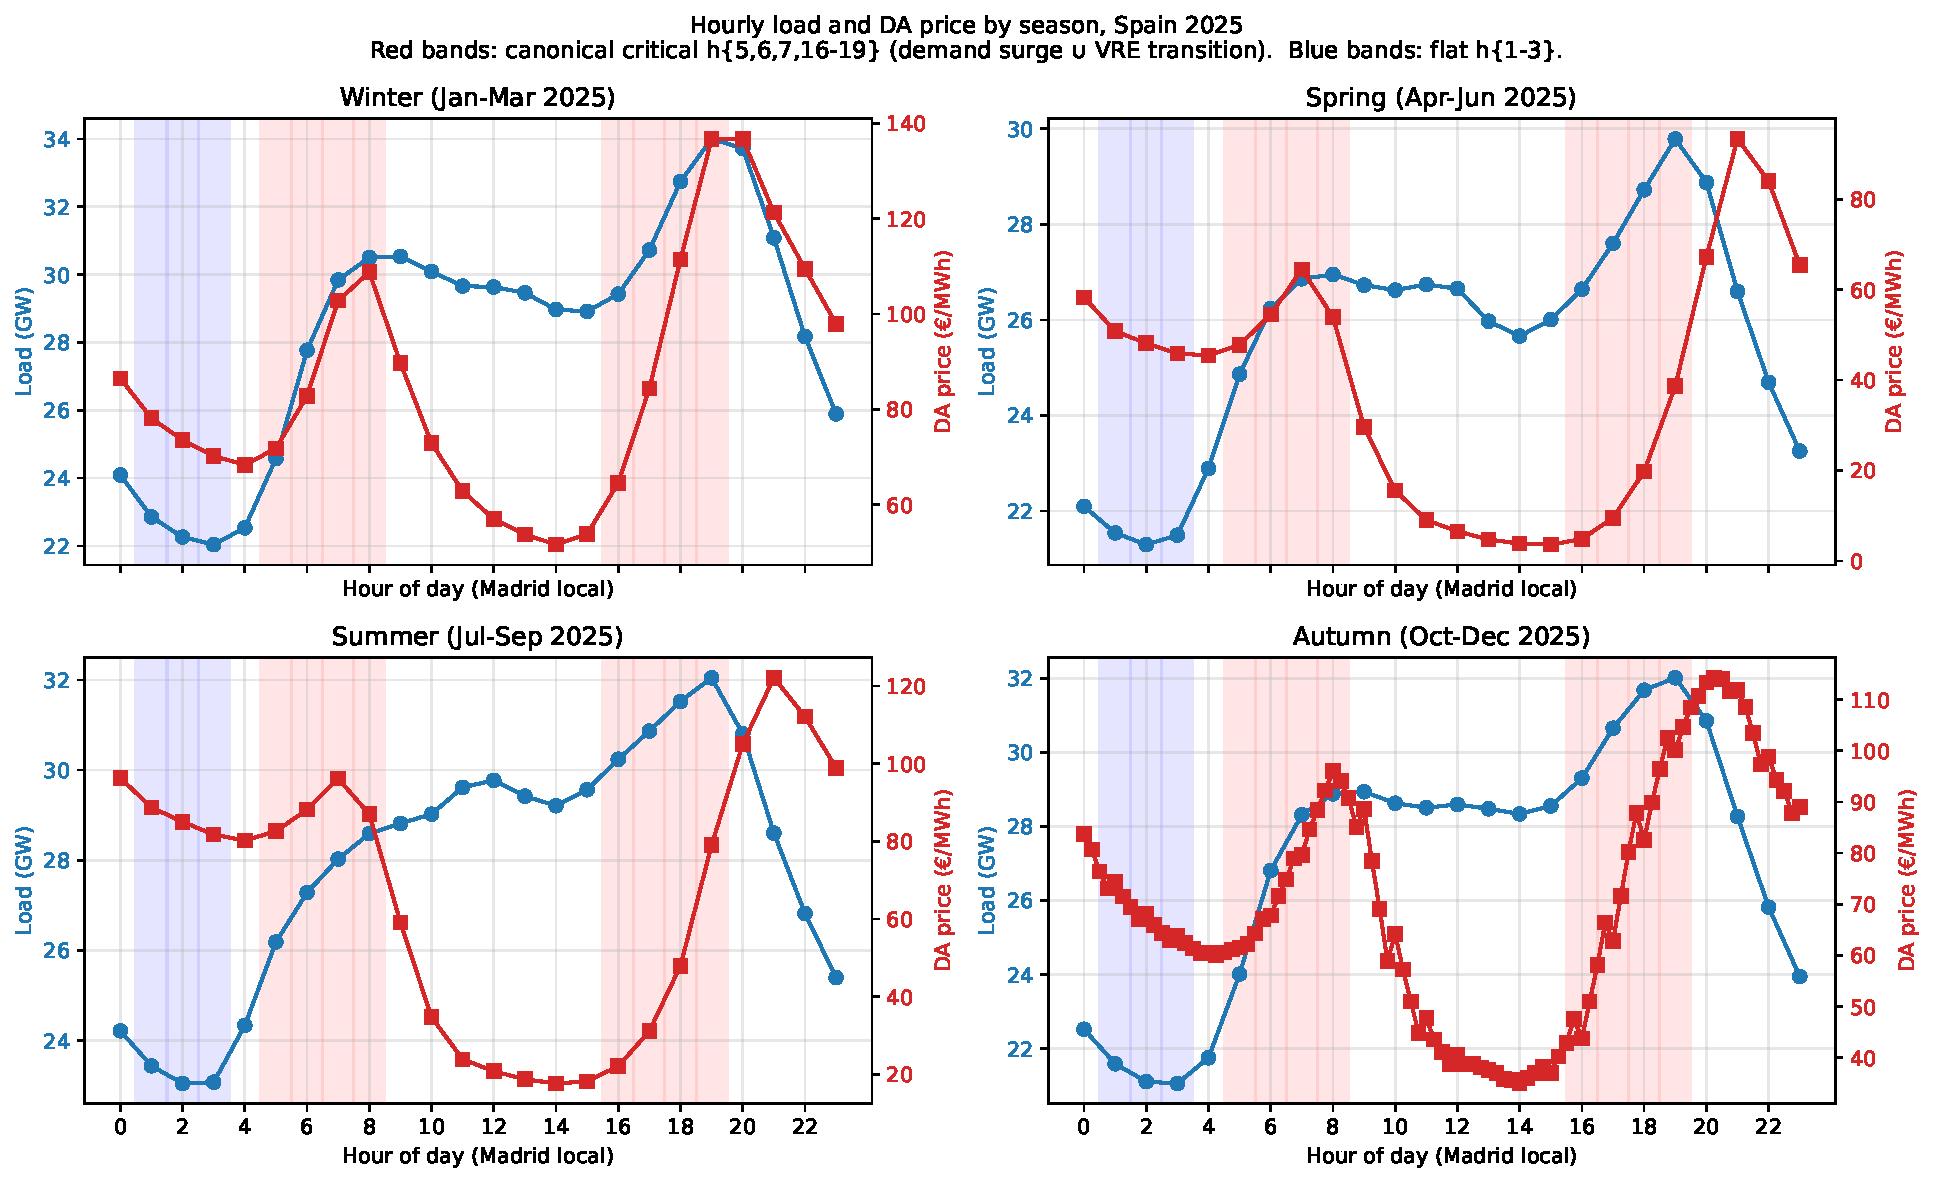
\includegraphics[width=0.95\textwidth]{fig_seasonal_critical_hours.pdf}
\caption{\textbf{Hourly load and DA price by season, Spain 2025.} Blue: demand; red: DA clearing price. Red bands: critical hours (05:00--09:00, 16:00--23:00); blue bands: flat hours (01:00--04:00). \emph{Note:} demand level is shown here for descriptive context only --- the formal classifier is $\sigma_{\text{within}}$ of residual demand (see Table~\ref{tab:hour_classification_full}), not demand level. The seasonal-stability of the within-day pattern is the relevant point. Reproduced from main paper \S2.1.}
\label{fig:hourclass_load}
\end{figure}

\begin{figure}[H]
\centering
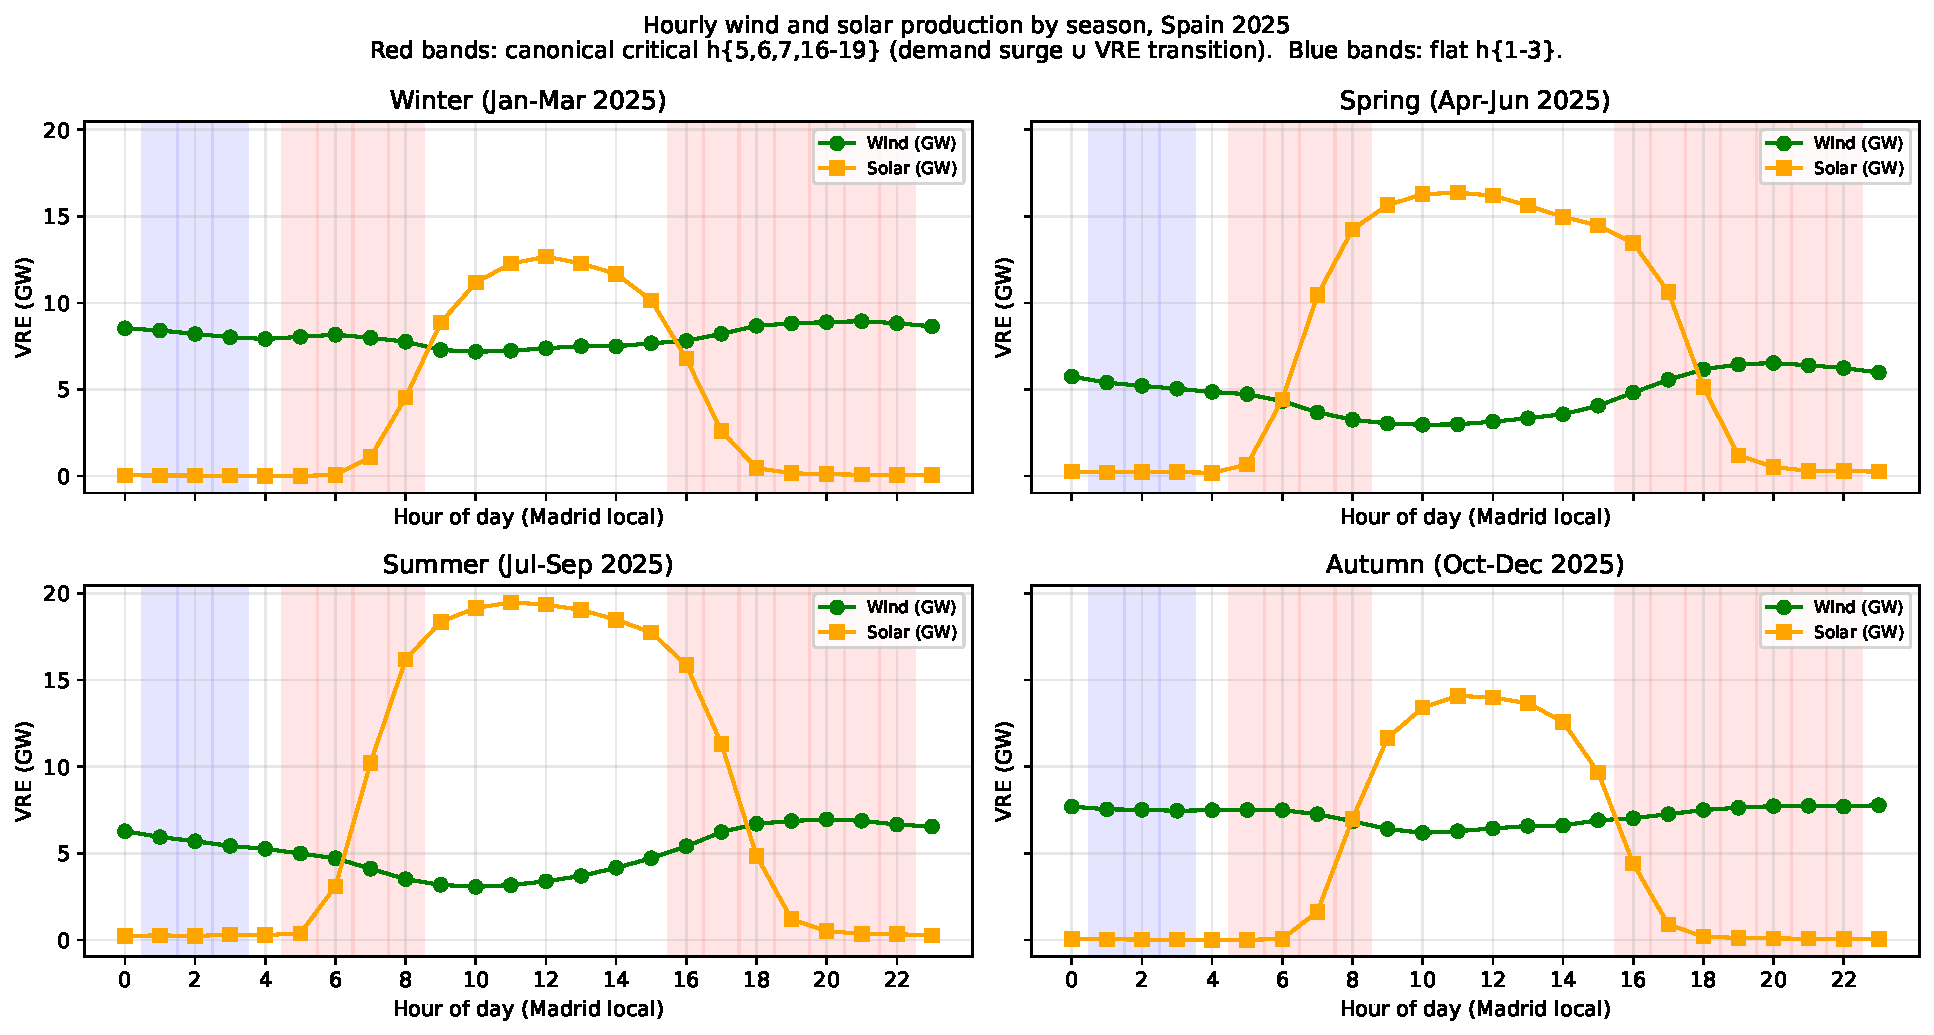
\includegraphics[width=0.95\textwidth]{fig_seasonal_vre.pdf}
\caption{\textbf{Hourly wind and solar production by season, Spain 2025.} Red bands: critical hours; blue bands: flat hours. Solar production concentrates in midday hours (11--14, white band between the two red bands) --- precisely the hours we exclude from the control. The high $\sigma_{\text{within}}$ in critical hours coincides with the morning solar rise and the evening solar fade (see Table~\ref{tab:hour_classification_full} for the per-hour values); the within-hour residual-demand swings in those windows are driven jointly by demand ramps and solar transitions. Reproduced from main paper \S2.1.}
\label{fig:hourclass_vre}
\end{figure}

% \paragraph{Source data.} \code{scripts/analysis/system/seasonal_critical_hours.py}; companion figure \code{fig_critical_hours_calibration.pdf} (variance of residual demand by hour, used to choose the crit-vs-flat boundaries) referenced in \code{paper.tex} \S2.1.


% =====================================================================
\section{Who price-sets}\label{sec:prov:pricesetter}
% =====================================================================

\subsection{For the day-ahead market}\label{sec:prov:pricesetter_da}

\paragraph{Method (compressed).} OMIE submits stepwise orders to EUPHEMIA: in-the-money fully accepted, out-of-the-money fully rejected, \textbf{at-the-money can be curtailed}. The price-setter is the unit whose at-MCP step is partially accepted. Operationally, with $q_{\text{below}}$ = sum of unit's bids strictly below MCP, $q_{\text{at}}$ = sum at MCP ($\pm 0.01$ EUR/MWh), and $q_{\text{assigned}}$ = unit's PDBC cleared MWh:
\[
 q_{\text{below}} + \varepsilon \;<\; q_{\text{assigned}} \;<\; q_{\text{below}} + q_{\text{at}} - \varepsilon
\]
Excluded: full acceptance ($q_{\text{assigned}} \ge q_{\text{below}} + q_{\text{at}}$, inframarginal at MCP) and curtailed-to-zero ($q_{\text{assigned}} \le q_{\text{below}}$, often MIC deactivation). Sources: clearing price from OMIE day-ahead clearing-price series; bid stack from OMIE day-ahead bid-detail and bid-header tables; cleared MWh from OMIE day-ahead programs. \textbf{Not} PDBF (bilaterals) or PHF (REE redispatch). Aggregations below MW-weighted by $q_{\text{at}}$ unless stated. Paradoxical rejection only applies to block orders (not in DET), so no separate filter is needed.
% Implementation: scripts/analysis/firm/price_setter_euphemia.py and scripts/analysis/firm/price_setter_deep_dive.py; outputs in results/regressions/firm/marginal_tech/ (incl. deep_dive/)

\emph{Naive vs corrected.} A naive rule that flags every unit with $p_{\text{bid}}=\text{MCP}$ (this is the rule CNMC uses in its annual market-supervision report, IS/DE/013/24; see Table~\ref{tab:cnmc_ccgt_metric} below) would pool all three cases; the direction of bias is tech-specific. For CCGT 2025Q4 critical, the CNMC-style 9.1\% becomes 2.7\% under partial-acceptance (most CCGT at-MCP steps are MIC-deactivated to zero); for 2024Q4 critical, 13.8\% becomes 18.1\%.

\paragraph{Side composition: sell-side dominates critical, buy-side dominates flat/midday in MTU15-DA.} Periods where at least one sell unit / at least one buy unit has an at-MCP step.

\begin{table}[H]
\centering\scriptsize
\setlength{\tabcolsep}{4pt}
\begin{tabular}{l r r r r r}
\toprule
Regime, hour-class & sell-only & buy-only & both & neither & $n$ periods \\
\midrule
DA15/ID15 Critical & 53\% & 25\% & 11\% & 11\% & 4{,}048 \\
DA15/ID15 \textbf{Flat} & 36\% & \textbf{42\%} & 10\% & 12\% & 1{,}104 \\
DA15/ID15 Midday & 28\% & \textbf{38\%} & 18\% & 17\% & 1{,}472 \\
DA60/ID15 post-blk Critical & 53\% & 19\% & 14\% & 14\% & 1{,}716 \\
DA60/ID15 post-blk Flat & 60\% & 17\% & 9\% & 13\% & 468 \\
3-sess Critical & 52\% & 21\% & 11\% & 15\% & 1{,}870 \\
\bottomrule
\end{tabular}
\caption{\textbf{At-MCP side presence}. ``neither'' = EUPHEMIA price-indeterminacy zone (MCP between bid steps, mid-point rule). In DA15/ID15 flat and midday, more periods are buy-side-only price-setting than sell-side-only.}
\label{tab:side_composition}
\end{table}

\paragraph{Sell-side price-setter shares by technology and regime (headline table).}

\begin{table}[H]
\centering\scriptsize
\caption{\textbf{Price-setter shares by technology and hour-class, across 5 reform-window regimes} (sell-side partial-acceptance, MW-weighted by $q_{\text{at}}$). C = Critical, F = Flat. Caveat: DA60/ID15 pre-blackout is 40 days only --- directional.}
\label{tab:pricesetter_tech_euphemia}
\setlength{\tabcolsep}{4pt}
\begin{tabular}{l r r r r r r r r r r}
\toprule
 & \multicolumn{2}{c}{\textbf{3-sess}} & \multicolumn{2}{c}{\textbf{ISP15-win}} & \multicolumn{2}{c}{\textbf{DA60/ID15 pre}} & \multicolumn{2}{c}{\textbf{DA60/ID15 post}} & \multicolumn{2}{c}{\textbf{DA15/ID15}} \\
\cmidrule(lr){2-3}\cmidrule(lr){4-5}\cmidrule(lr){6-7}\cmidrule(lr){8-9}\cmidrule(lr){10-11}
Tech & C & F & C & F & C & F & C & F & C & F \\
\midrule
Wind & 28.3 & 17.9 & 37.8 & 63.9 & 47.5 & 70.9 & 29.6 & 17.3 & 29.3 & 53.0 \\
Solar PV & 17.7 & 0.0 & 1.4 & 0.0 & 20.6 & 0.0 & 29.9 & 0.0 & 7.7 & 0.0 \\
Hydro pump & 10.4 & 13.3 & 17.0 & 2.7 & 2.2 & 10.8 & 8.0 & 19.3 & 28.4 & 13.0 \\
Hydro & 11.9 & 36.1 & 19.6 & 10.9 & 2.7 & 1.7 & 9.4 & 21.5 & 23.7 & 20.0 \\
Nuclear & 12.5 & 20.2 & 4.2 & 6.5 & 15.6 & 13.5 & 7.9 & 5.5 & 4.4 & 3.3 \\
CCGT & 8.0 & 8.9 & 17.2 & 11.1 & 0.8 & 0.0 & 6.2 & 33.1 & 2.7 & 2.0 \\
Cogen & 3.0 & 0.3 & 0.1 & 0.1 & 2.5 & 0.1 & 2.1 & 0.1 & 0.5 & 0.9 \\
Other RES & 3.9 & 1.5 & 0.6 & 0.2 & 3.4 & 0.8 & 3.1 & 1.2 & 1.2 & 2.2 \\
Import & 0.8 & 0.8 & 0.5 & 3.1 & 0.0 & 0.0 & 0.0 & 0.0 & 0.5 & 3.3 \\
\bottomrule
\end{tabular}
\end{table}

\paragraph{Cross-check: CNMC's broader marginal-tech metric.} The Spanish regulator CNMC publishes an analogous metric in its annual market-supervision report (\emph{Informe de supervisión del mercado peninsular mayorista al contado de electricidad. A\~no 2023}, IS/DE/013/24, 28 Jan 2025), where it states for example that \emph{``los ciclos combinados se convierten en la tecnolog\'ia marginal en un porcentaje elevado de las horas (21,7\% cuota ciclos, 43,3\% cuota renovable en septiembre''} of 2023 (\S2.5.3, p.~51). CNMC's metric counts a unit as marginal whenever its highest-accepted sell tranche lands at MCP, \emph{regardless of whether the at-MCP step is curtailed or fully accepted}. Our partial-acceptance metric above is strictly tighter (it requires the at-MCP step to be \emph{strictly partially} accepted). Table~\ref{tab:cnmc_ccgt_metric} reports the CNMC-style version of the CCGT row of Table~\ref{tab:pricesetter_tech_euphemia} for our 5 reform windows; the two metrics give the same qualitative ranking but the CNMC version is mechanically larger.
% Implementation: scripts/analysis/firm/marginal_tech_cnmc_style.py; output in results/regressions/firm/marginal_tech/cnmc_marginal_tech_shares.csv

\begin{table}[H]
\centering\scriptsize
\caption{\textbf{CCGT marginal-tech share, CNMC-style vs partial-acceptance.} CNMC-style = \% of MW-weighted votes where the rank-1 accepted sell tranche (highest $p_{\text{bid}}$ with $p_{\text{bid}}\le\text{MCP}$) belongs to a CCGT unit; ties at rank 1 split the vote equally across units. This matches the share concept used in CNMC IS/DE/013/24 Cuadro 11 (p.~81). Partial-acceptance = the strict EUPHEMIA-aware rule of Table~\ref{tab:pricesetter_tech_euphemia}. C = Critical, F = Flat, M = Midday. CNMC's reported September~2023 figure for CCGT (21.7\%, peninsular monthly average) is roughly the order of magnitude of our 3-sess critical-hour CCGT share under the CNMC-style metric (13.1\%) and the ISP15-win critical-hour share (14.1\%).}
\label{tab:cnmc_ccgt_metric}
\setlength{\tabcolsep}{4pt}
\begin{tabular}{l r r r r r r}
\toprule
 & \multicolumn{3}{c}{\textbf{CNMC-style (rank-1 at MCP)}} & \multicolumn{3}{c}{\textbf{Partial-acceptance (ours)}} \\
\cmidrule(lr){2-4}\cmidrule(lr){5-7}
Regime & C & F & M & C & F & M \\
\midrule
3-sess (Jun--Nov 2024) & 13.1 & 5.9 & 6.9 & 8.0 & 8.9 & --- \\
ISP15-win (Dec24--Mar25) & 14.1 & 13.0 & 14.7 & 17.2 & 11.1 & --- \\
DA60/ID15 pre-blk (Mar19--Apr27) & 2.2 & 0.0 & 0.7 & 0.8 & 0.0 & --- \\
DA60/ID15 post-blk (Apr28--Sep) & 11.1 & 20.5 & 0.4 & 6.2 & 33.1 & --- \\
\textbf{DA15/ID15 (Oct--Dec 2025)} & 9.1 & 9.3 & 1.9 & 2.7 & 2.0 & --- \\
\bottomrule
\end{tabular}
\end{table}

\emph{Why the two metrics diverge.} The largest gap is DA15/ID15 critical (9.1 CNMC vs 2.7 ours): under MTU15-DA, most CCGT at-MCP steps are \emph{MIC-deactivated to zero} ($q_{\text{assigned}}\le q_{\text{below}}$), which the CNMC rule still counts as ``marginal'' but the partial-acceptance rule does not. The DA60/ID15 post-blackout flat row goes the other way (20.5 CNMC vs 33.1 ours), because in that regime a couple of Endesa CCGT units (SROQ2, PGR5) submit single-block full-nameplate tranches at MCP that get \emph{partially} accepted (driving up the partial-acceptance share) but are not the rank-1 marginal step in many of those periods. Both metrics agree that DA60/ID15 pre-blackout has near-zero CCGT marginal presence and that DA15/ID15 critical is much lower than ISP15-win or 3-sess.

\paragraph{CCGT firm-level: GN never price-sets, IB and GE swap dominance.} Within the CCGT column above, who owns the at-MCP step?

\begin{table}[H]
\centering\scriptsize
\setlength{\tabcolsep}{5pt}
\begin{tabular}{l l r r r r r}
\toprule
Regime & Hour-class & IB & GE & GN & HC & OTHER \\
\midrule
3-sess & Critical & \textbf{60} & 31 & 0 & 0 & 8 \\
3-sess & Flat & 16 & \textbf{50} & 0 & 0 & 25 \\
ISP15-win & Critical & 35 & \textbf{57} & 0 & 0 & 5 \\
ISP15-win & Flat & 2 & \textbf{74} & 0 & 3 & 20 \\
DA60/ID15 post-blk & Critical & 31 & \textbf{69} & 0 & 0 & 0 \\
DA60/ID15 post-blk & Flat & 19 & \textbf{80} & 0 & 0 & 0 \\
\textbf{DA15/ID15} & Critical & \textbf{65} & 29 & 0 & 6 & 0 \\
\textbf{DA15/ID15} & Flat & \textbf{80} & 0 & 6 & 14 & 0 \\
\bottomrule
\end{tabular}
\caption{\textbf{Per-firm shares within the CCGT price-setter pool} (\% of CCGT $q_{\text{at}}$). \textbf{GN's CCGT bid stack is so heavily concentrated at scarcity prices ($\ge 500$ EUR/MWh) that GN essentially never lands at MCP}. IB and GE alternate as the dominant CCGT price-setter. The 33.1\% CCGT flat-hour figure in DA60/ID15 post-blackout is 80\% GE.}
\label{tab:ccgt_by_firm}
\end{table}

\emph{Top price-setting units in DA15/ID15 (for context).} MUEL (Iberdrola's Muela del Cortes pump-storage) is the workhorse: 496 events / $\sim$5.5 events per day. Other Iberdrola hydro (DUER 201, TAJO 171, SIL 130 events) and the IBEVD11 wind aggregator (153 events, but $\sim 1{,}613$ MW per event = 247 GW total $q_{\text{at}}$) dominate the top 7. Endesa's MLTG pump-storage (164 events) is the only non-Iberdrola unit in the top 5.

\paragraph{Reading across regimes (synthesis).}
\begin{itemize}
\item \textbf{Wind is the largest sell-side price-setter} in almost every cell (18--71\% MW share). RE-Mercado aggregator portfolios systematically land at-the-money; 70--99\% of wind/solar/cogen at-MCP events involve a single block at MCP with no in-the-money bids (the deep-dive companion data). CCGT, hydro, and pump-storage instead use true stacks (24--34\% single-block).
\item \textbf{Iberdrola dominates the marginal MW in DA15/ID15} (top-1 firm-share $\approx 65\%$ critical, $80\%$ flat; firm HHI $> 4{,}000$), through Hydro pump (MUEL), Hydro (DUER, TAJO, SIL), and the IBEVD11 wind aggregator.
\item \textbf{CCGT's share fluctuates strongly across regimes}: 8\% (3-sess) $\to$ 17\% (ISP15-win) $\to$ 0.8\% (DA60/ID15 pre-blk, tiny window) $\to$ 6\% / 33\% (flat) (DA60/ID15 post-blk) $\to$ 3\% (DA15/ID15) in critical hours. The 33\% flat-hour spike is 80\% GE-owned, driven by $\sim 2$ units (SROQ2, PGR5 --- both Endesa) submitting single full-nameplate ($\sim$360 MW) tranches at MCP (MIC-reservation style); cell-count-weighted alternative is 17\%.
\item \textbf{GN does not partial-accept at MCP, but is strategically active within-hour.} GN's CCGT bid mass sits at scarcity prices ($\geq 500$ EUR/MWh) and rarely lands at MCP for partial acceptance, but the bid \emph{shape} across the 4 within-hour quarters is the largest of any CCGT firm in terms of median price shift (see Table~\ref{tab:within_hour_shaping} below). Direct inspection of BES4 (GN) confirms: on 2025-10-15 hour 18, Q1 is binary (1 EUR / 1000 EUR), Q2 the same, Q3 adds a small near-clearing tier, Q4 has a full 10-step ladder at 81--97 EUR/MWh.
\item \textbf{Solar PV} dominates midday post-MTU15-DA ($35.1\%$, see CSV) and the negative/zero-MCP scarcity bin ($40$--$65\%$). CCGT never sets the price at $\text{MCP}\le 0$.
\item \textbf{Buy-side price-setters} are dominated by pump-load demand bids ($46$--$84\%$) and retailer demand bids ($14$--$53\%$). In DA15/ID15 flat hours, buy-side sets the price about $42\%$ of periods (vs $36\%$ sell-side).
\item \textbf{Cross-regime CCGT symmetry} (simple TTF/gas-shock falsifier) holds in 3-sess (8.0 vs 8.9) and DA15/ID15 (2.7 vs 2.0), but breaks in ISP15-win (17.2 vs 11.1) and DA60/ID15 post-blk (6.2 vs 33.1).
\end{itemize}

\subsection{For the intraday markets}\label{sec:prov:pricesetter_ida}

\paragraph{Method.} Identical partial-acceptance rule as \S\ref{sec:prov:pricesetter_da}, with three data substitutions: clearing price from OMIE intraday-auction clearing-price series (per session $\times$ period), bid stack from OMIE intraday-auction bid-detail data $+$ OMIE intraday-auction bid-header data (sell-side, latest version, pools across the 3 IDA sessions per day), cleared MWh per unit from OMIE intraday-auction programs per unit. Matched-period share is $26$--$32\%$ across regimes (similar to DA).
% Implementation: scripts/analysis/firm/price_setter_euphemia_ida.py; outputs in results/regressions/firm/marginal_tech/price_setter_euphemia_ida_*.csv

\begin{table}[H]
\centering\scriptsize
\caption{\textbf{IDA price-setter shares by technology, hour-class, and regime} (at-the-money partial-acceptance, sell side), MW-weighted by $q_{\text{at}}$. C = Critical, F = Flat. Shares sum to 100 per (regime, hour-class).}
\label{tab:pricesetter_ida}
\setlength{\tabcolsep}{4pt}
\begin{tabular}{l r r r r r r r r r r}
\toprule
 & \multicolumn{2}{c}{\textbf{3-sess}} & \multicolumn{2}{c}{\textbf{ISP15-win}} & \multicolumn{2}{c}{\textbf{DA60/ID15 pre}} & \multicolumn{2}{c}{\textbf{DA60/ID15 post}} & \multicolumn{2}{c}{\textbf{DA15/ID15}} \\
\cmidrule(lr){2-3}\cmidrule(lr){4-5}\cmidrule(lr){6-7}\cmidrule(lr){8-9}\cmidrule(lr){10-11}
Tech & C & F & C & F & C & F & C & F & C & F \\
\midrule
Wind & 35.5 & 15.7 & 24.8 & 40.2 & 52.6 & 53.8 & 37.8 & 18.8 & 31.9 & 42.4 \\
CCGT & 14.1 & 29.2 & 16.1 & 15.3 & 3.1 & 2.8 & 9.7 & 23.1 & \textbf{24.2} & \textbf{32.6} \\
Hydro pump & 12.9 & 23.4 & 17.2 & 2.2 & 2.5 & 13.0 & 6.2 & 26.1 & 14.0 & 3.8 \\
Solar PV & 10.5 & 0.0 & 1.7 & 0.1 & 20.3 & 0.0 & 22.8 & 0.0 & 7.5 & 0.1 \\
Hydro & 6.4 & 15.9 & 18.4 & 23.4 & 4.4 & 3.4 & 5.6 & 15.6 & 10.0 & 10.6 \\
Retailer & 10.2 & 6.2 & 10.4 & 12.1 & 5.3 & 7.5 & 7.3 & 11.8 & 5.7 & 5.2 \\
Nuclear & 2.7 & 3.2 & 0.0 & 0.0 & 1.0 & 13.8 & 2.5 & 1.3 & 2.5 & 0.0 \\
Other RES & 1.0 & 1.1 & 1.7 & 0.0 & 3.1 & 0.7 & 2.4 & 0.2 & 0.6 & 0.4 \\
\bottomrule
\end{tabular}
\end{table}

\paragraph{Reading the IDA table.}
\begin{itemize}
\item \textbf{CCGT is much more active as an IDA price-setter than as a DA price-setter in DA15/ID15.} Critical-hour CCGT IDA share is \textbf{24.2\%} (vs \textbf{2.7\%} in DA); flat-hour CCGT IDA share is \textbf{32.6\%} (vs \textbf{2.0\%} in DA). A factor of $\sim 9$--$16$. The natural reading: CCGTs sit out of DA (bidding above the clearing price; see also the $q_1$-drop story in Part B, \S\ref{sec:prov:q1_drop}) and re-enter via IDA, where they now systematically clear at the marginal step.
\item \textbf{Wind dominates IDA too}, but less than in DA: $32\%$ IDA critical share in DA15/ID15 vs $29\%$ DA critical share. Wind aggregators play in both markets.
\item \textbf{CCGT IDA share collapsed in the DA60/ID15 pre-blackout window} (3.1\% critical) but recovered post-blackout (9.7\%) and grew to 24.2\% under DA15/ID15. The post-MTU15-DA jump is striking and consistent with a DA-to-IDA strategic substitution.
\item \textbf{Retailer (buy-side, IDA)} sets the price 5--12\% of IDA critical-hour mass — comparable order to DA. Buy-side matters in IDA too.
\end{itemize}


% =====================================================================
\section{Bid-curve shape: per-curve functionals and pairwise divergences}\label{sec:prov:dw_decomp}
% =====================================================================

\noindent We measure bid-curve shape with two conceptually distinct families of statistics, and keep them separate throughout.
\begin{itemize}\setlength{\itemsep}{3pt}
\item \textbf{Family 1 --- per-curve functionals.} A functional maps a \emph{single} bid curve to a scalar, $T: f \mapsto T(f) \in \mathbb{R}$; no comparison between curves enters its definition. Cross-regime, cross-firm and cross-hour reading is then done by comparing the \emph{values} $T(f)$ across curves. This family holds the price spread $\sigma_p$ and the effective tranche count $N_{\text{eff}}$ (\S\ref{sec:prov:per_curve_def}), and the functional-PCA level/tilt scores $\xi_{ik}$ of \S\ref{sec:prov:fpca} --- the score $\xi_{ik} = \langle f_i - \bar f,\, \phi_k\rangle$ is itself a per-curve functional, a shape coordinate of the single curve $f_i$. \textbf{This is the primary descriptive object}: it asks what one bid curve looks like, and how that value moves across regimes.
\item \textbf{Family 2 --- pairwise divergences.} A divergence is a statistic of \emph{two} curves, $D(f_i, f_j)$: it does not summarise either curve on its own, it measures how far apart they are. This family holds $D_w$ and its $\Delta p$ / $\Delta q$ channel decomposition (\S\ref{sec:prov:dw_decomp_def}). We use it for one comparison only --- a unit's four within-hour quarter curves against each other --- as a within-hour-shaping diagnostic, secondary to Family~1.
\end{itemize}
\noindent The distinction is the one the advisor asked for: characterise each bid curve by its own value (Family~1), rather than by divergences between curves (Family~2). Family~2 is retained only because the within-hour quarter comparison has no single-curve analogue.

% =====================================================================
\subsection{Family 1 --- per-curve functionals: $\sigma_p$ and $N_{\text{eff}}$}\label{sec:prov:per_curve_def}
% =====================================================================

\noindent For each (unit, date, market-period) sell bid curve, restricted to the strategic band $|p - \text{MCP}| \le 50$ EUR/MWh, we compute two scalars:
\begin{itemize}\setlength{\itemsep}{2pt}
\item \textbf{Price functional --- price spread $\sigma_p$}: the MW-weighted standard deviation of the in-band tranche prices (EUR/MWh). It measures how much the unit \emph{varies its price} across the MW it offers near the clearing price. A single flat block $\Rightarrow \sigma_p = 0$; a graded ladder spanning the band $\Rightarrow \sigma_p$ large.
\item \textbf{Quantity functional --- effective tranche count $N_{\text{eff}}$}: the inverse Herfindahl of the tranche MW shares, $N_{\text{eff}} = (\sum_t q_t)^2 / \sum_t q_t^2$. It measures how the unit \emph{splits its quantity}: $N_{\text{eff}} = 1$ means all in-band MW sits in one block, larger $N_{\text{eff}}$ means the MW is divided into more comparable pieces.
\end{itemize}
\noindent Both are per-curve and require no curve-to-curve comparison, and are computed on the \emph{raw} bid curve (seasonality is handled at the aggregation step, by reading the values within calendar-matched windows). The two decouple: a unit can split into many tranches at nearly one price (high $N_{\text{eff}}$, low $\sigma_p$) or place two blocks far apart (low $N_{\text{eff}}$, high $\sigma_p$). The fPCA scores of \S\ref{sec:prov:fpca} are the third member of this family --- a multivariate per-curve functional that lets the data choose the modes of shape variation rather than fixing them a priori.

% =====================================================================
\subsection{Family 2 --- pairwise divergences: $D_w$, $\Delta p$, $\Delta q$}\label{sec:prov:dw_decomp_def}
% =====================================================================

\paragraph{$D_w$, in full.}
Let cell $(f, u, d, h)$ index a firm $f$, unit $u$, date $d$, clock-hour $h$. The hour partitions into 4 quarters $q \in \{1,2,3,4\}$. In quarter $q$ the unit submits a multiset of price-quantity sell tranches with $p\in[\underline p, \overline p] \subset \mathbb{R}$ (Spanish SDAC: $\underline p = -500$, $\overline p = 4{,}000$ EUR/MWh; negative bids are admissible) and $x>0$ (MWh, energy for the quarter-slot). Let $c_{d,h}$ be the hour-mean clearing price (justified below) and fix a strategic half-band of half-width $h = 50$ EUR/MWh (justified below) around it. \textbf{We work throughout with band-restricted supply curves}: $N_q$ is the number of \emph{distinct} prices submitted in quarter $q$ \emph{within} $[c-h, c+h]$, and $x_{qk}$ is the sum of quantities at $p_{qk}$. The band-local quarter-$q$ supply curve is the right-continuous step function
\[
 S_q(p) \;=\; \sum_{k=1}^{N_q} x_{qk}\,\mathbf{1}\{p_{qk}\le p\}, \qquad p \in [c-h, c+h],
\]
with $S_q(c-h) = 0$ and $S_q(c+h) = M_q$ (the band-mass of quarter $q$ --- the total MWh offered \emph{anywhere inside} the band $[c-h, c+h]$, not the offer at the maximum-price threshold). Infra-marginal mass below $c-h$ is excluded by construction: $D_w$ measures the within-band \emph{shape} of supply across quarters, not infra-marginal level offsets.

For two quarters $i, j$, the 1-D Wasserstein-1 distance is the $L^1$ area between cumulative curves, equivalently the $L^1$ distance between (extended) quantile functions:
\[
 W^{\text{band}}_1(S_i, S_j) \;=\; \int_{c-h}^{c+h}\!\big|S_i(p)-S_j(p)\big|\,dp \;=\; \int_{0}^{\max(M_i, M_j)}\!\big|S_i^{-1}(Q)-S_j^{-1}(Q)\big|\,dQ,
\]
where $S_q^{-1}(Q) = c+h$ for $Q > M_q$ pads the smaller curve to common total mass (Vallender, 1973). To isolate variation near the clearing price, weight by an (unnormalized) Epanechnikov-shape kernel:
\[
 K_h(p-c) \;=\; \max\!\left\{0,\;1 - \!\left(\frac{p-c}{h}\right)^{\!2}\right\}, \quad K_h \in [0,1], \quad K_h(c)=1,
\]
\[
 D^{(i,j)}_w \;=\; \int_{c-h}^{c+h}\! K_h(p-c)\,\big|S_i(p)-S_j(p)\big|\,dp \;\le\; W^{\text{band}}_1.
\]
$D_w$ has units EUR (quantity in MWh times price in EUR/MWh).

\paragraph{Why $c$ = hour-mean clearing price.} The band isolates the strategic pricing region --- the range where the unit's bids had a non-trivial probability of clearing. We centre on $c_{d,h}$, the hour-mean of the four within-hour quarter clearing prices, so the band is common to all 6 quarter-pairs in a cell; a quarter-specific centre would measure shifts of the reference, not of the curve.

\paragraph{Why $h = 50$ EUR/MWh.} Spanish DA clearing prices in 2024--25 sit in the 50--150 EUR/MWh range, so a $\pm 50$ band captures bid mass within roughly one ``clearing-price width'' of clearing --- the region where placement matters for being on the margin --- while excluding strategic high-cap bids (800--3{,}000 EUR/MWh). A sensitivity sweep $h \in \{20, 50, 100, 200\}$ preserves the qualitative ranking (GN dominant on $\Delta q$, GE leaning on $\Delta p$, IB/HC negligible, flat hours $\approx 0$); $h=50$ is the working choice.

\paragraph{Cell-level aggregation: mean across the 6 within-hour pairs.}
A cell has $\binom{4}{2} = 6$ pairwise dissimilarities $D_w^{(i,j)}$, aggregated to a cell-level statistic by the \emph{mean} $D^{\text{cell}}_w = \tfrac{1}{6}\sum_{i<j} D^{(i,j)}_w$. For the binary flag $D^{\text{cell}}_w > 0$ the choice of mean vs.\ max is irrelevant (a cell has any pair $>0$ iff mean $>0$ iff max $>0$); for conditional intensity we report the mean, which reads as the typical-pair within-hour shift.

\paragraph{Decomposition into price and quantity channels.}
We split the within-band variation into a price channel and a quantity channel:
\[
 \Delta q_{ij} \;=\; |M_i - M_j|\;\;[\text{MWh}],
 \qquad
 \Delta p_{ij} \;=\; \frac{1}{\min(M_i, M_j)}\int_{0}^{\min(M_i, M_j)}\!\!\big|S_i^{-1}(Q) - S_j^{-1}(Q)\big|\,dQ\;\;[\text{EUR/MWh}].
\]
$\Delta p$ captures the mean price shift on the common-mass portion --- a price-only adjustment with band-mass totals held fixed, in EUR/MWh. $\Delta q$ captures band-mass mismatch --- a quantity-only adjustment with prices on the common-mass portion held fixed, in MWh. Cell-level $\Delta p$, $\Delta q$ are the mean over the 6 pairs, consistent with the $D_w$ aggregation above.

\paragraph{Consistency and the $\Delta q$ caveat.} Extending the smaller quantile function to common mass $M_j$ and splitting the Wasserstein integral at $Q=M_i$ gives the bound
\[
 D^{(i,j)}_w \;\le\; W^{\text{band}}_1 \;\le\; \Delta p_{ij}\,M_i + 2h\,\Delta q_{ij},
\]
exact in the two limiting cases: $M_i = M_j \Rightarrow$ all variation on the price channel; coinciding quantile functions on common mass $\Rightarrow$ all variation on the quantity channel. \textbf{Read $\Delta p$ and $\Delta q$ as channel indicators (active/inactive, and which dominates), not as additive contributions} --- empirically the bound is loose by $\sim 13\times$ (the extra band-mass sits near the top of the band). Raw $\Delta q$ in MWh is also coarse on its own: 10 MWh of asymmetric mass is large in a 20 MWh cell and negligible in a 500 MWh one, so we lean on the active/inactive distinction rather than the raw level.

% =====================================================================
\subsection{Bid graphs by tech, firm, and within-hour quarter}\label{sec:prov:bid_graphs}

\noindent The figures in this subsection display the aggregate within-hour quarter bid (or demand) curves, broken down by firm and hour-class. Each curve overlays the mean DA (or IDA) clearing price as a reference so the strategic-band $|p - c| \le 50$ EUR/MWh region is visible. Aggregation: average across $\sim$92 dates per (firm, hour, quarter) cell for the DA Oct--Dec 2025 window. Day-specific quarter dispersion is smoothed by this construction; the per-curve price and quantity metrics in \S\ref{sec:prov:dw_tables} are the right quantitative complement.

\paragraph{CCGT (DA): aggregate per-firm quarter curves, critical vs flat.}
\textit{Reading} (\textbf{mixed}). The aggregate construction smooths per-day strategic shaping; the per-curve metric distributions at the end of \S\ref{sec:prov:dw_tables} are the right systematic measure.

\begin{figure}[H]
\centering
\begin{subfigure}[t]{0.49\textwidth}
\centering
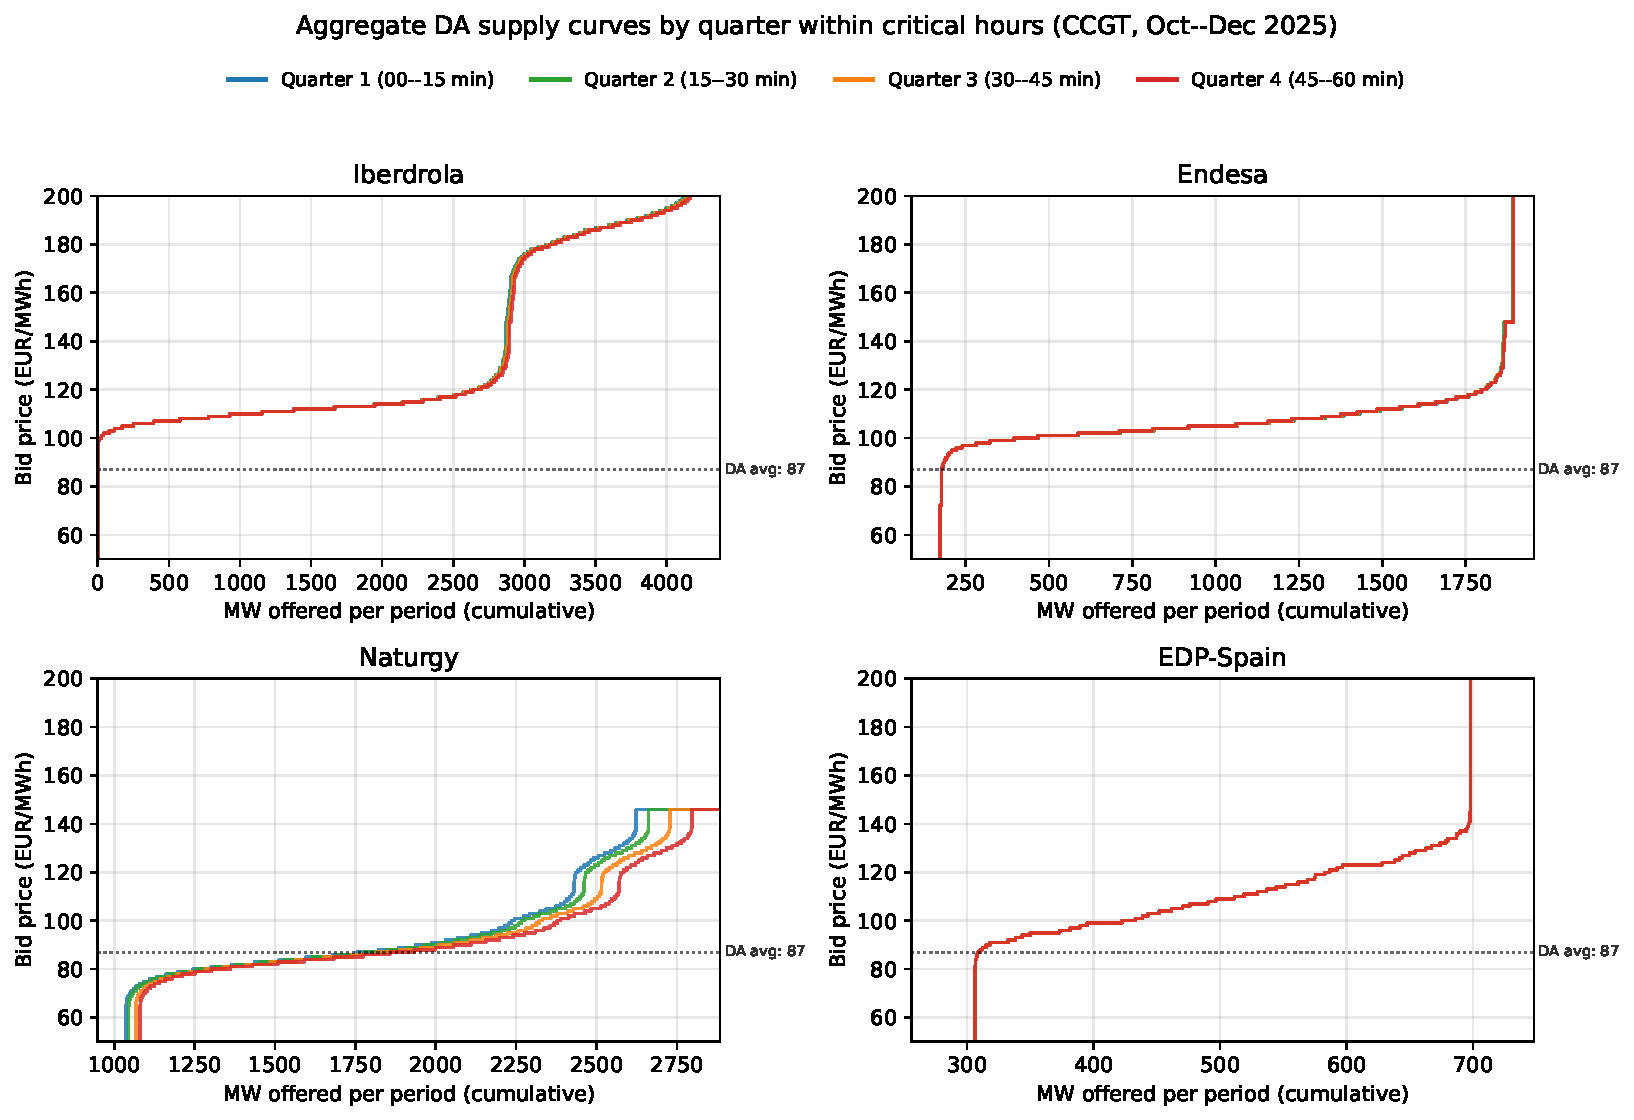
\includegraphics[width=\textwidth]{fig_per_firm_bid_curves_quarters_ccgt.pdf}
\caption{Critical hours (05:00--09:00, 16:00--23:00)}
\end{subfigure}\hfill
\begin{subfigure}[t]{0.49\textwidth}
\centering
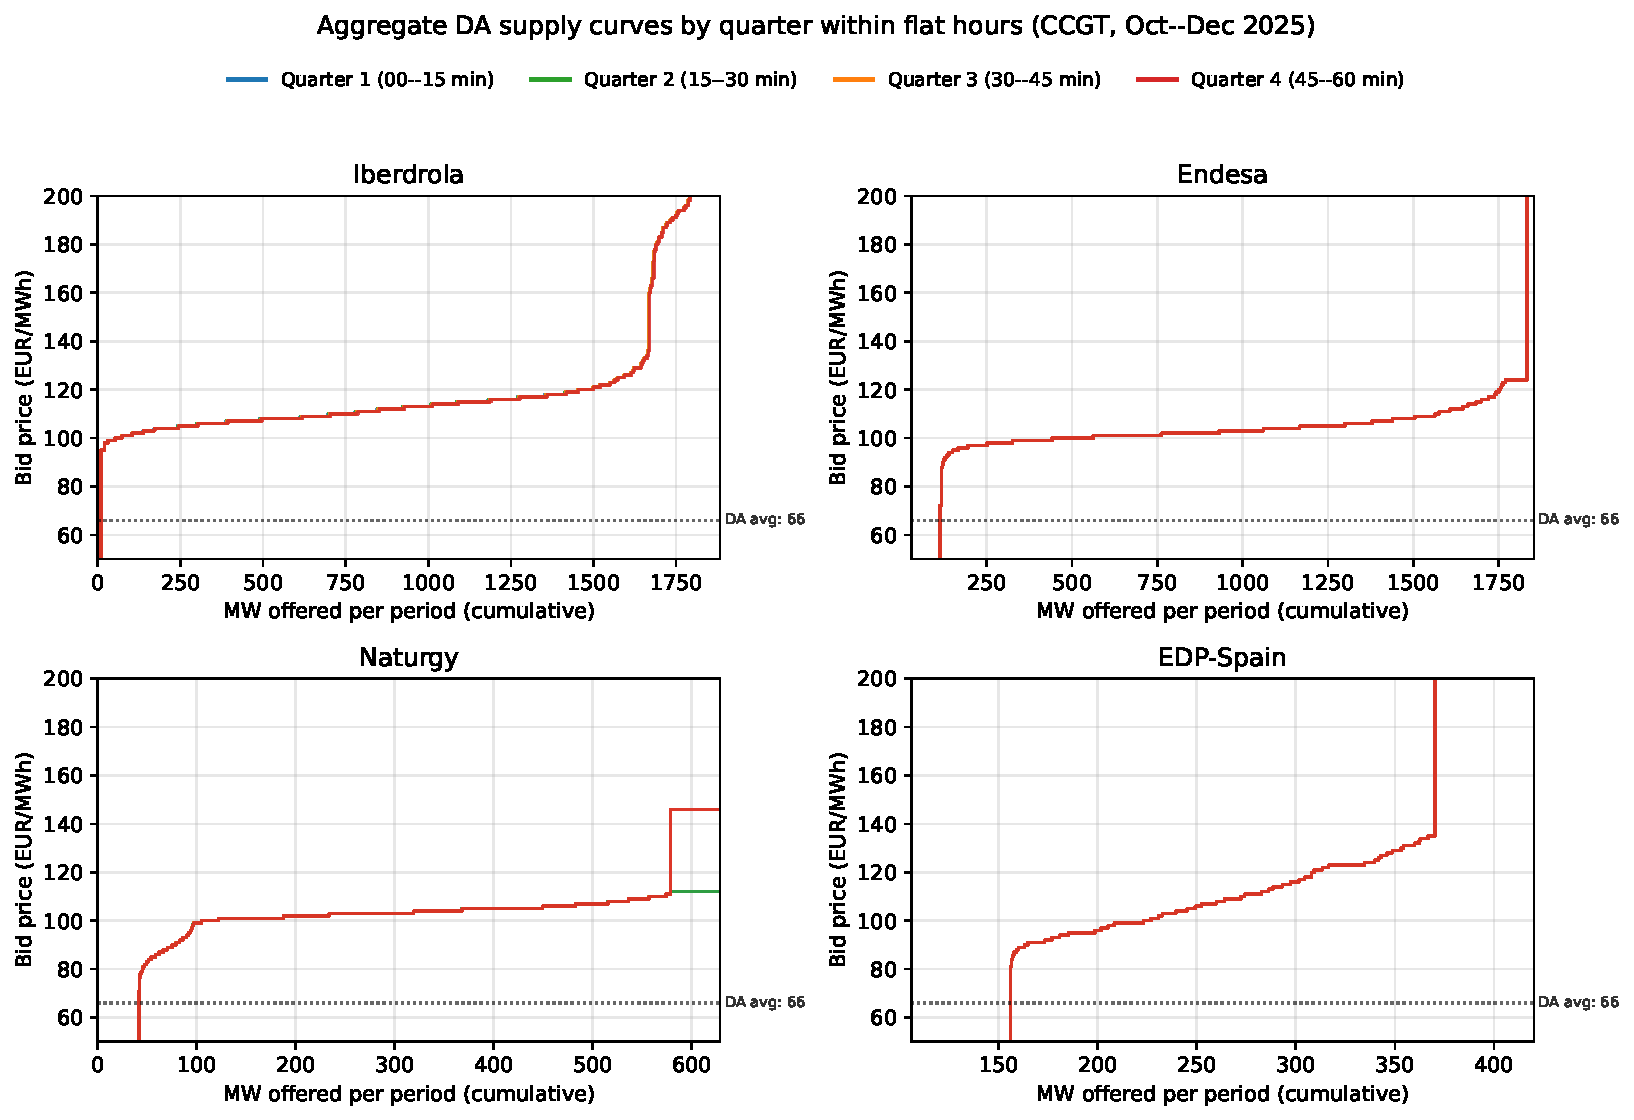
\includegraphics[width=\textwidth]{fig_per_firm_bid_curves_quarters_ccgt_flat.pdf}
\caption{Flat hours (01:00--04:00) --- falsification}
\end{subfigure}
\caption{Aggregate DA supply curves by quarter, CCGT, Oct--Dec 2025. Aggregated across $\sim$92 dates per (firm, hour, quarter) cell; day-specific quarter dispersion is smoothed in this visual.}
\end{figure}

\noindent In the post-MTU15-DA window the IDA per-firm pattern matches DA (dispersion concentrated in Naturgy, visible only in critical hours); the IDA-side figure is not reproduced separately.

\paragraph{Compact multi-tech grids: firm $\times$ tech $\times$ quarter, all techs side by side.}\label{sec:prov:compact_grids}
The grids below stack rows = Big-4 firms (Iberdrola, Endesa, Naturgy, EDP-Spain) against columns = techs (CCGT, Hydro, Nuclear, Wind, Solar PV). Each panel overlays the 4 within-hour quarter supply curves (Q1 blue $\to$ Q4 red) with the mean DA / IDA clearing price as a dotted horizontal line. \emph{Reading}: the same-quarter overlap in flat hours is the falsification; visible quarter spread in critical hours is the strategic signal.

\begin{figure}[H]
\centering
\begin{subfigure}[t]{0.49\textwidth}
\centering
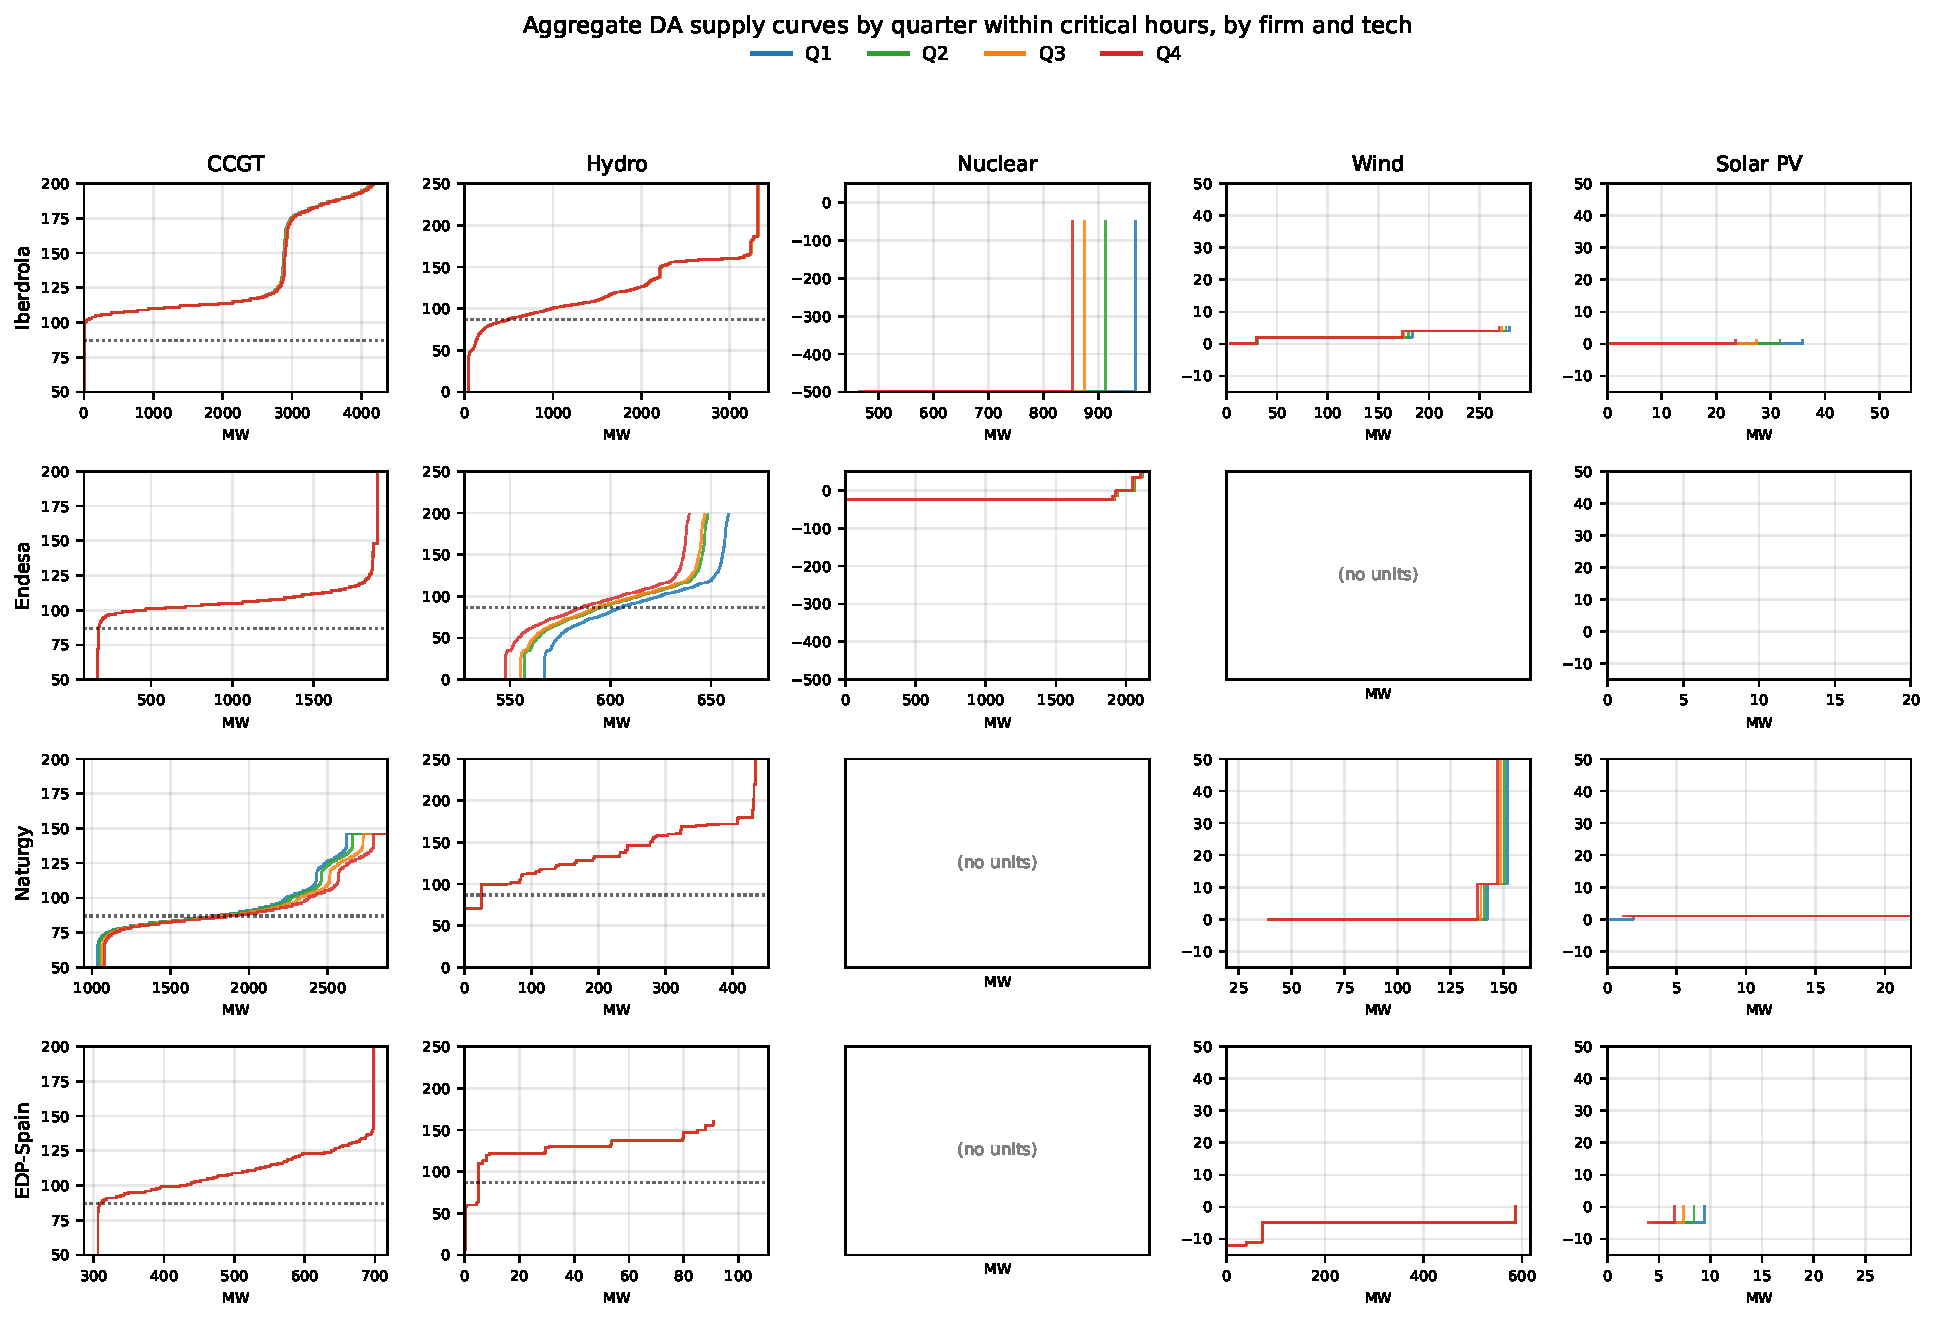
\includegraphics[width=\textwidth]{fig_bid_curves_grid_per_quarter.pdf}
\caption{DA, critical hours.}
\end{subfigure}\hfill
\begin{subfigure}[t]{0.49\textwidth}
\centering
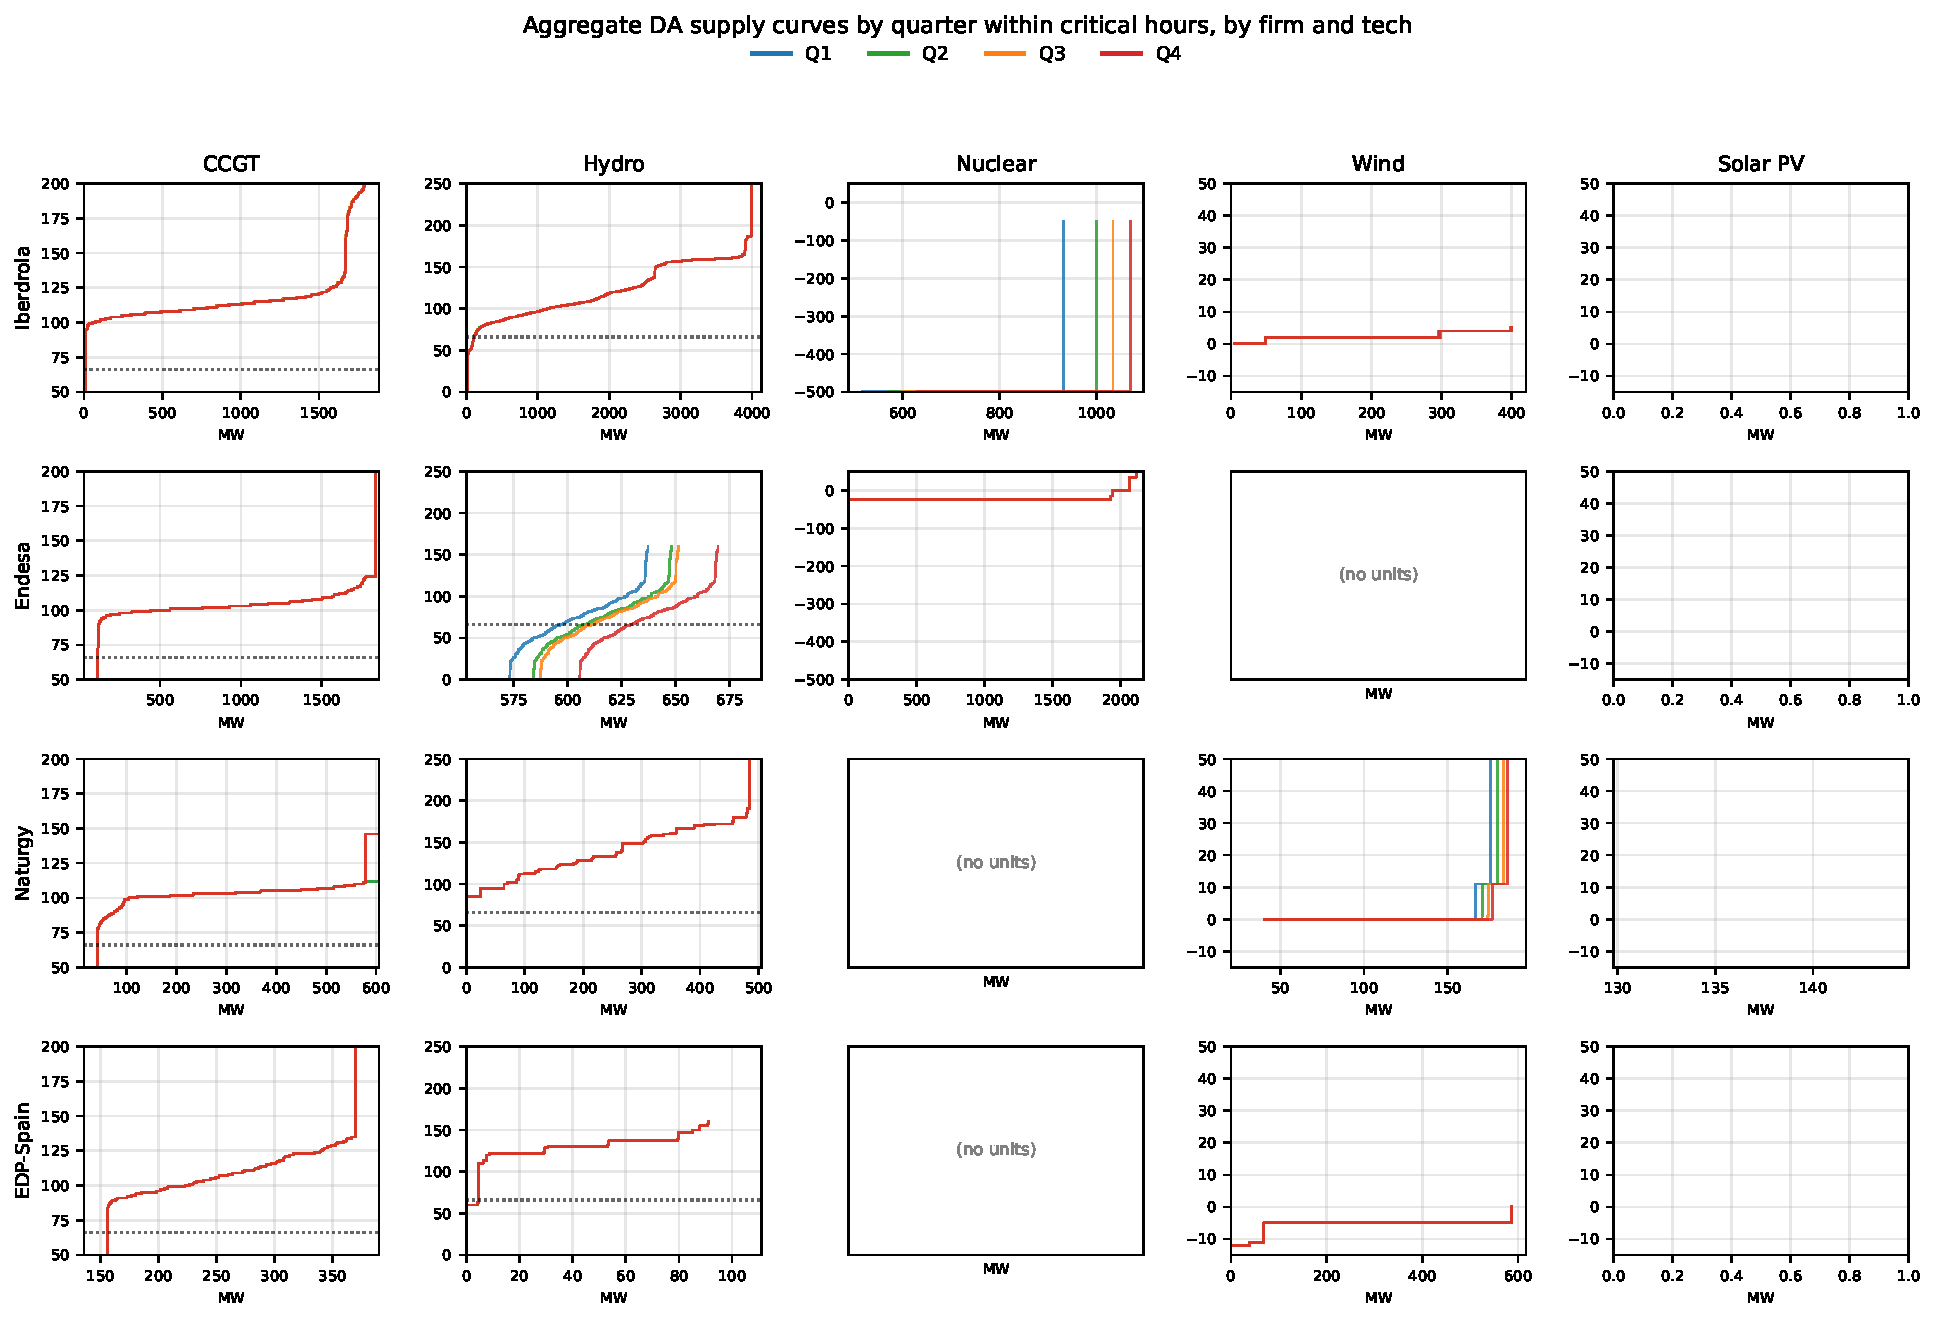
\includegraphics[width=\textwidth]{fig_bid_curves_grid_per_quarter_flat.pdf}
\caption{DA, flat hours --- falsification.}
\end{subfigure}
\caption{\textbf{DA compact grid (firms $\times$ techs $\times$ quarter), DA15/ID15.} Quarter overlap in flat hours is essentially complete; critical-hour spread is visible for GN CCGT and Endesa Hydro.}
\end{figure}

\begin{figure}[H]
\centering
\begin{subfigure}[t]{0.49\textwidth}
\centering
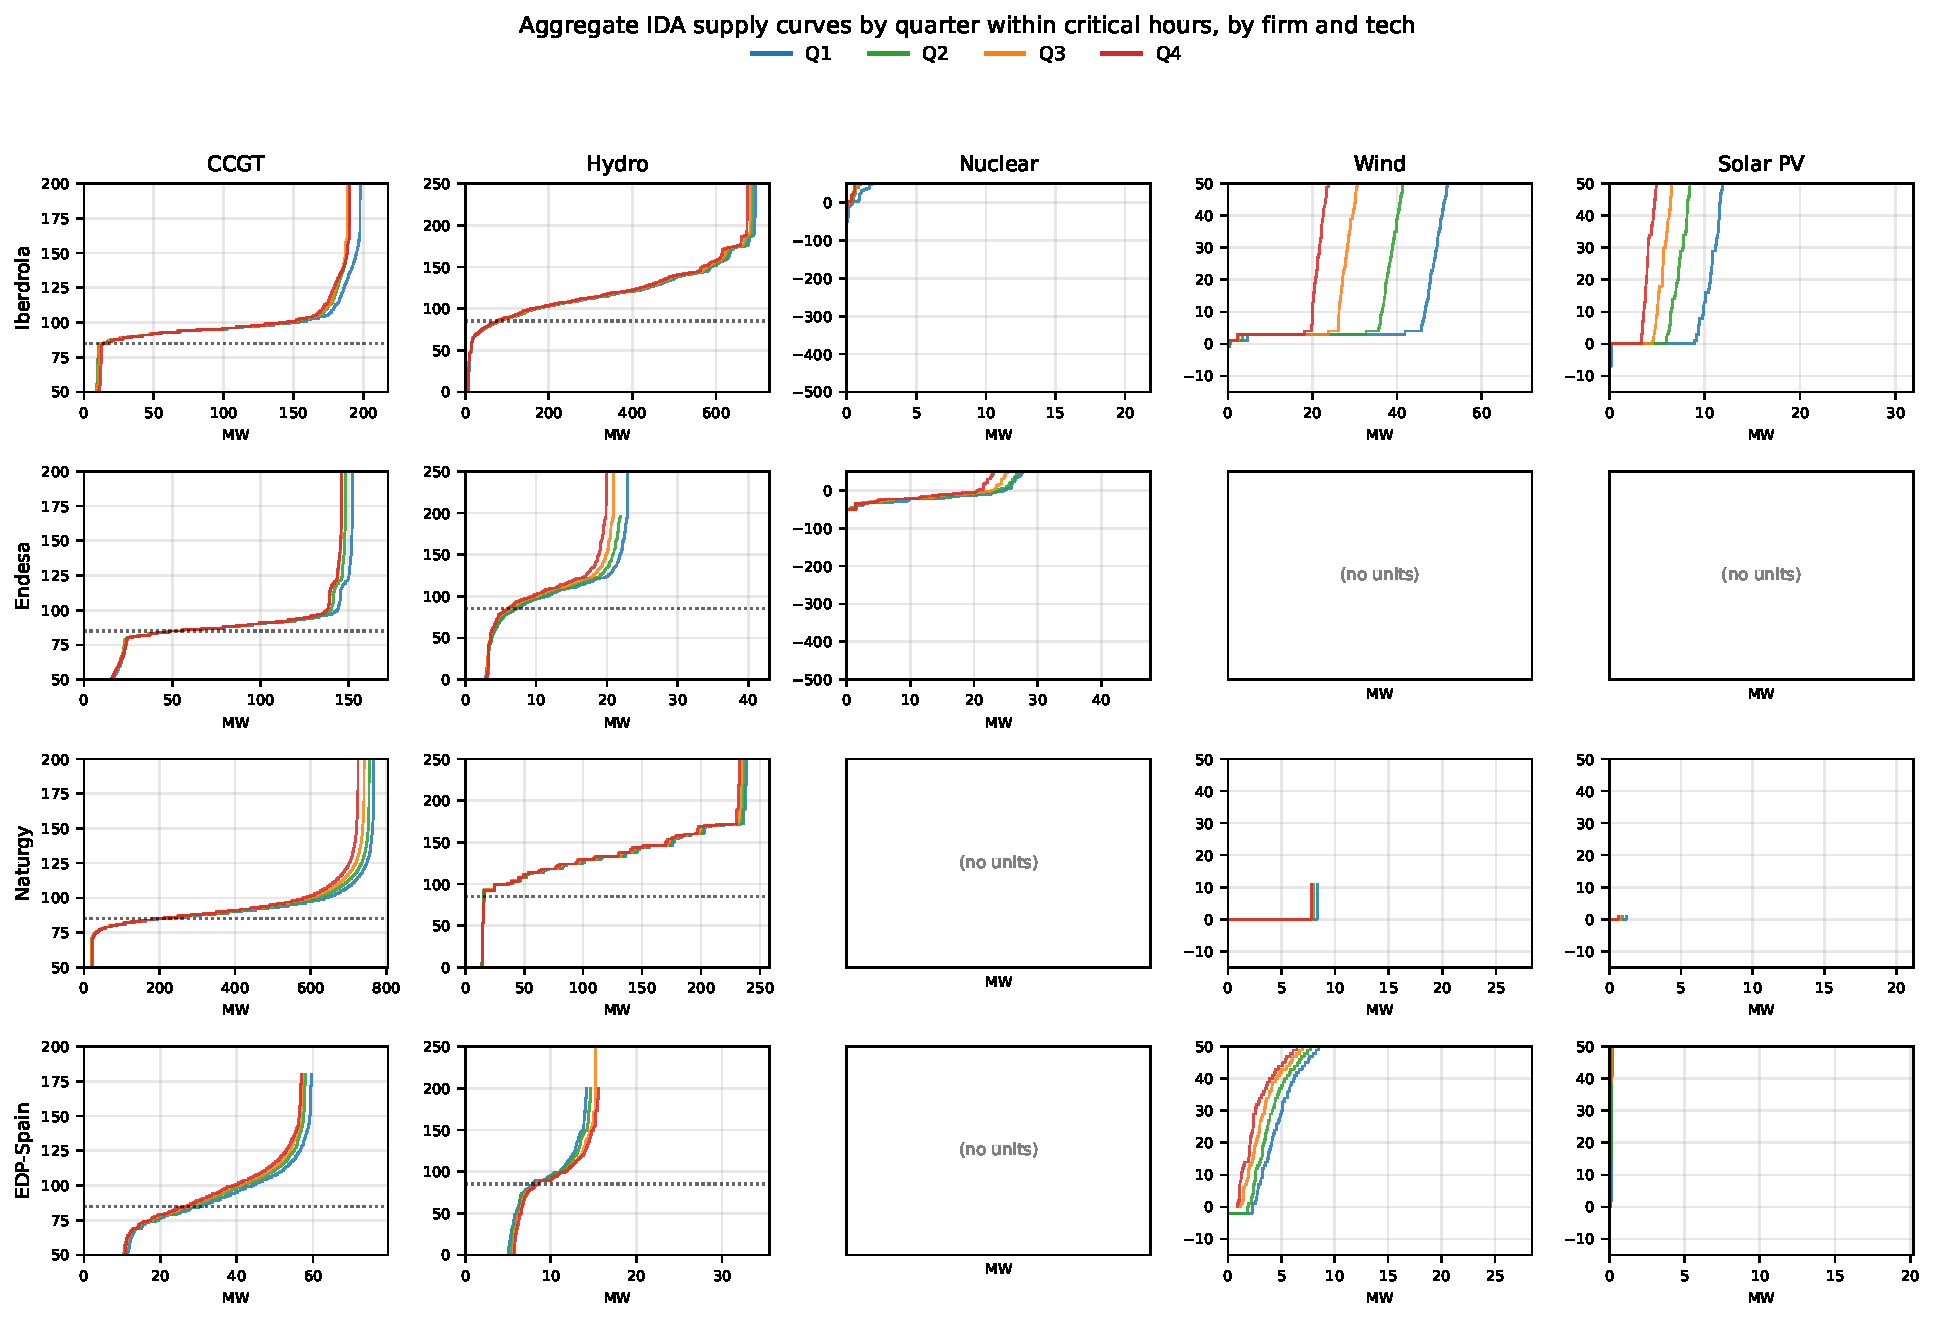
\includegraphics[width=\textwidth]{fig_bid_curves_grid_per_quarter_ida.pdf}
\caption{IDA, critical hours.}
\end{subfigure}\hfill
\begin{subfigure}[t]{0.49\textwidth}
\centering
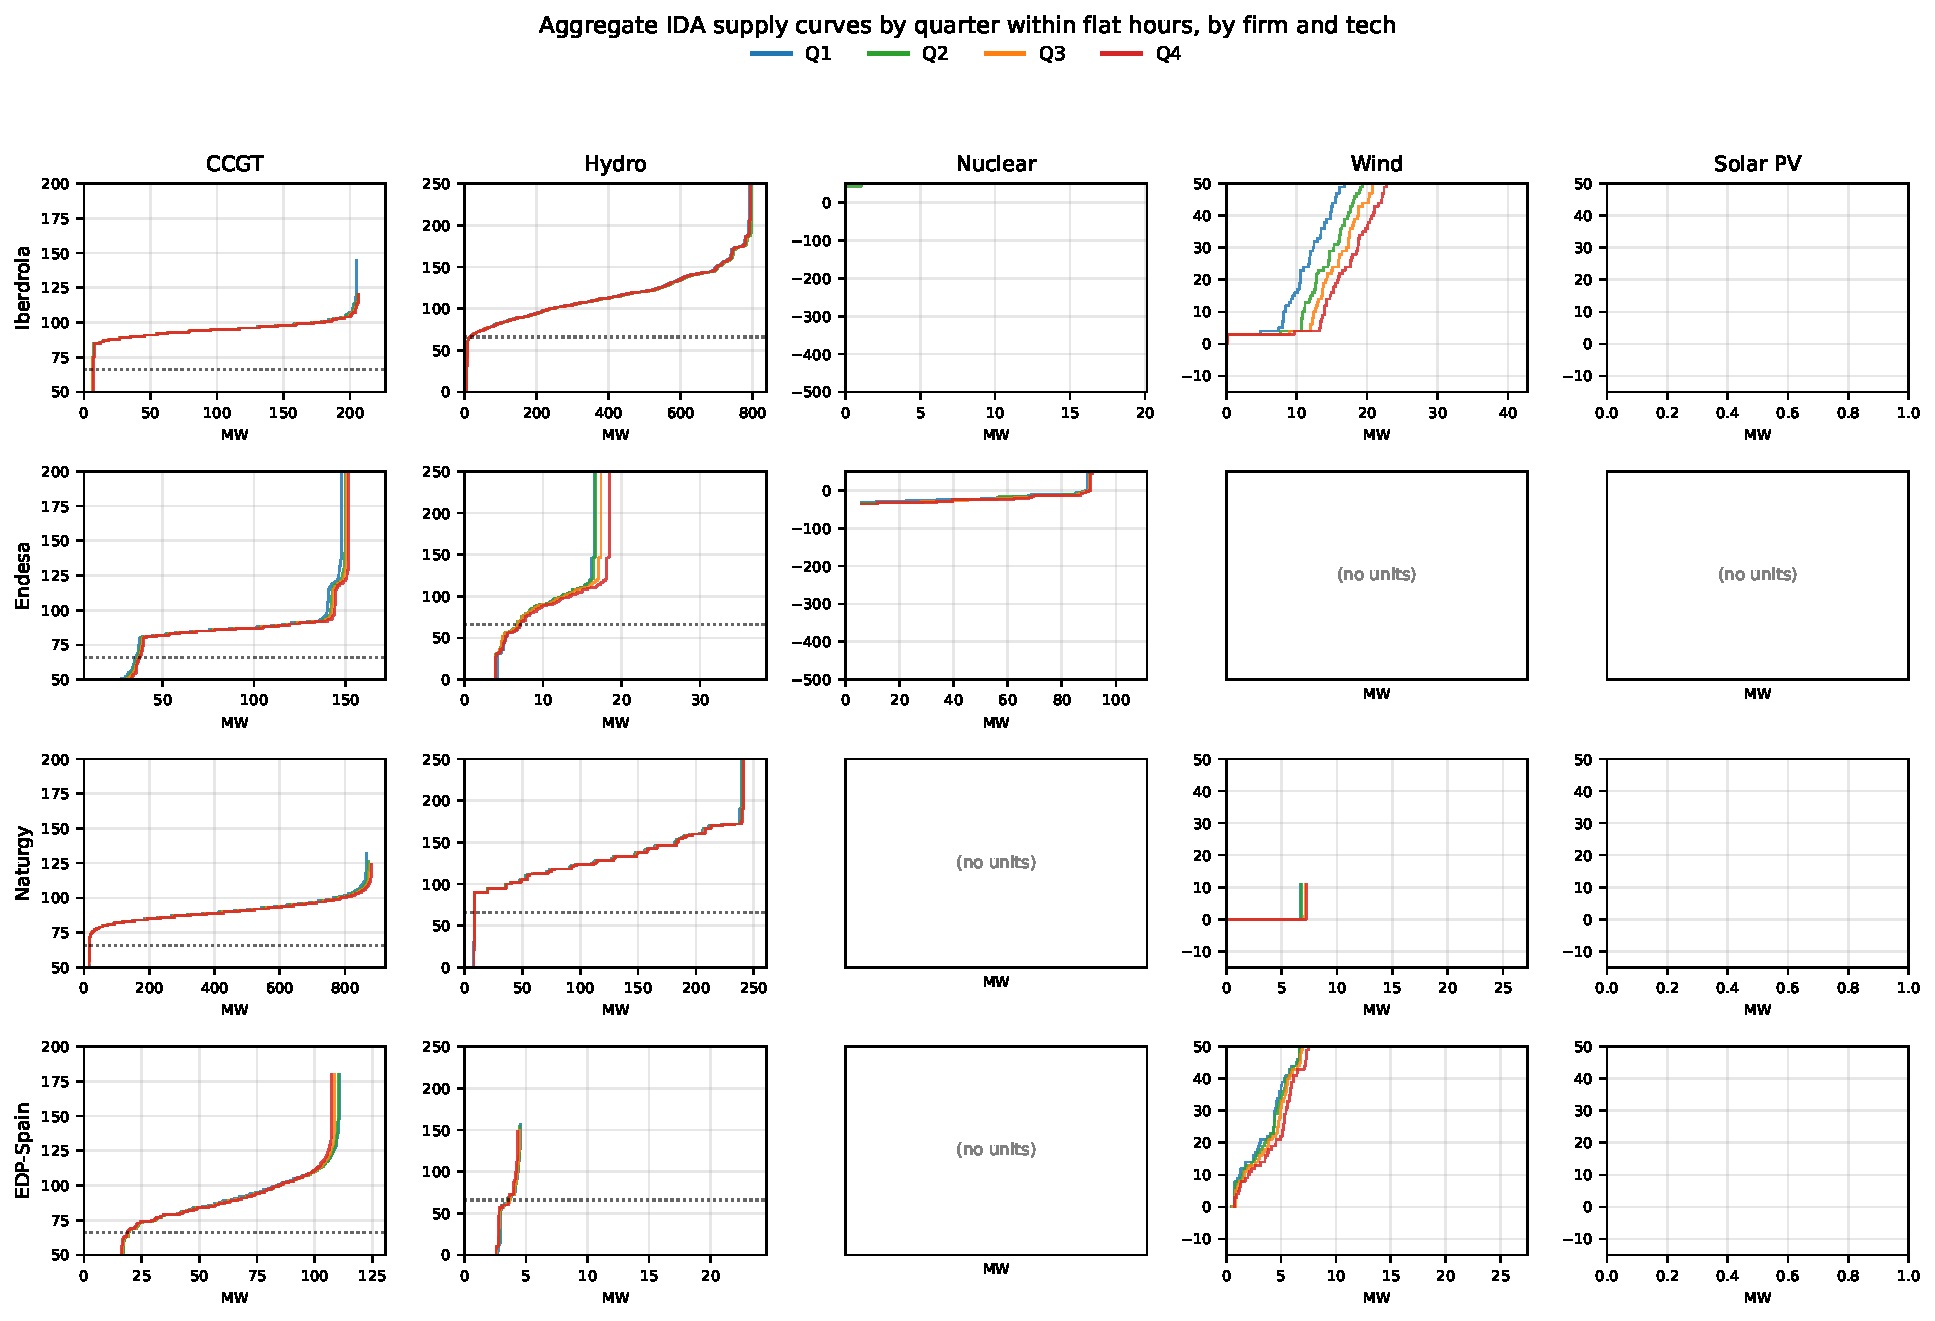
\includegraphics[width=\textwidth]{fig_bid_curves_grid_per_quarter_ida_flat.pdf}
\caption{IDA, flat hours.}
\end{subfigure}
\caption{\textbf{IDA compact grid (firms $\times$ techs $\times$ quarter), DA15/ID15.} IDA-side analogue; quarter spread on the supply side is more visible than in DA.}
\end{figure}

\begin{figure}[H]
\centering
\begin{subfigure}[t]{0.49\textwidth}
\centering
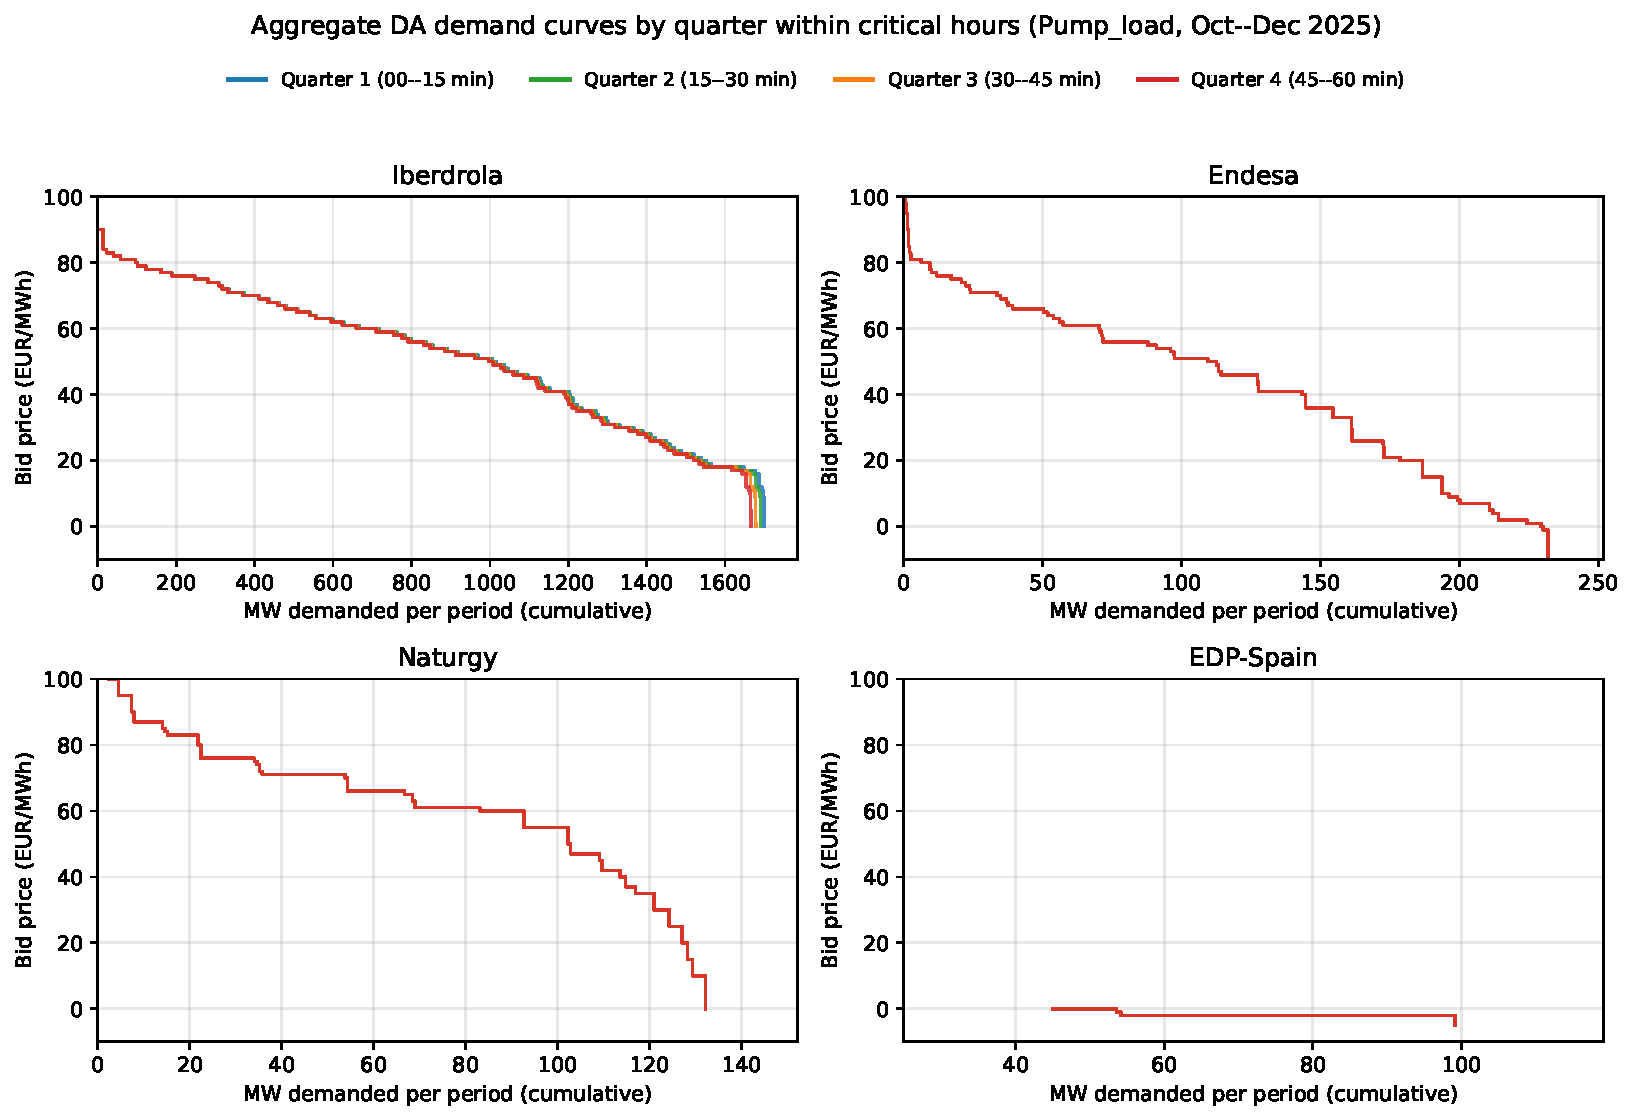
\includegraphics[width=\textwidth]{fig_per_firm_demand_curves_quarters_pump_load.pdf}
\caption{DA, critical hours}
\end{subfigure}\hfill
\begin{subfigure}[t]{0.49\textwidth}
\centering
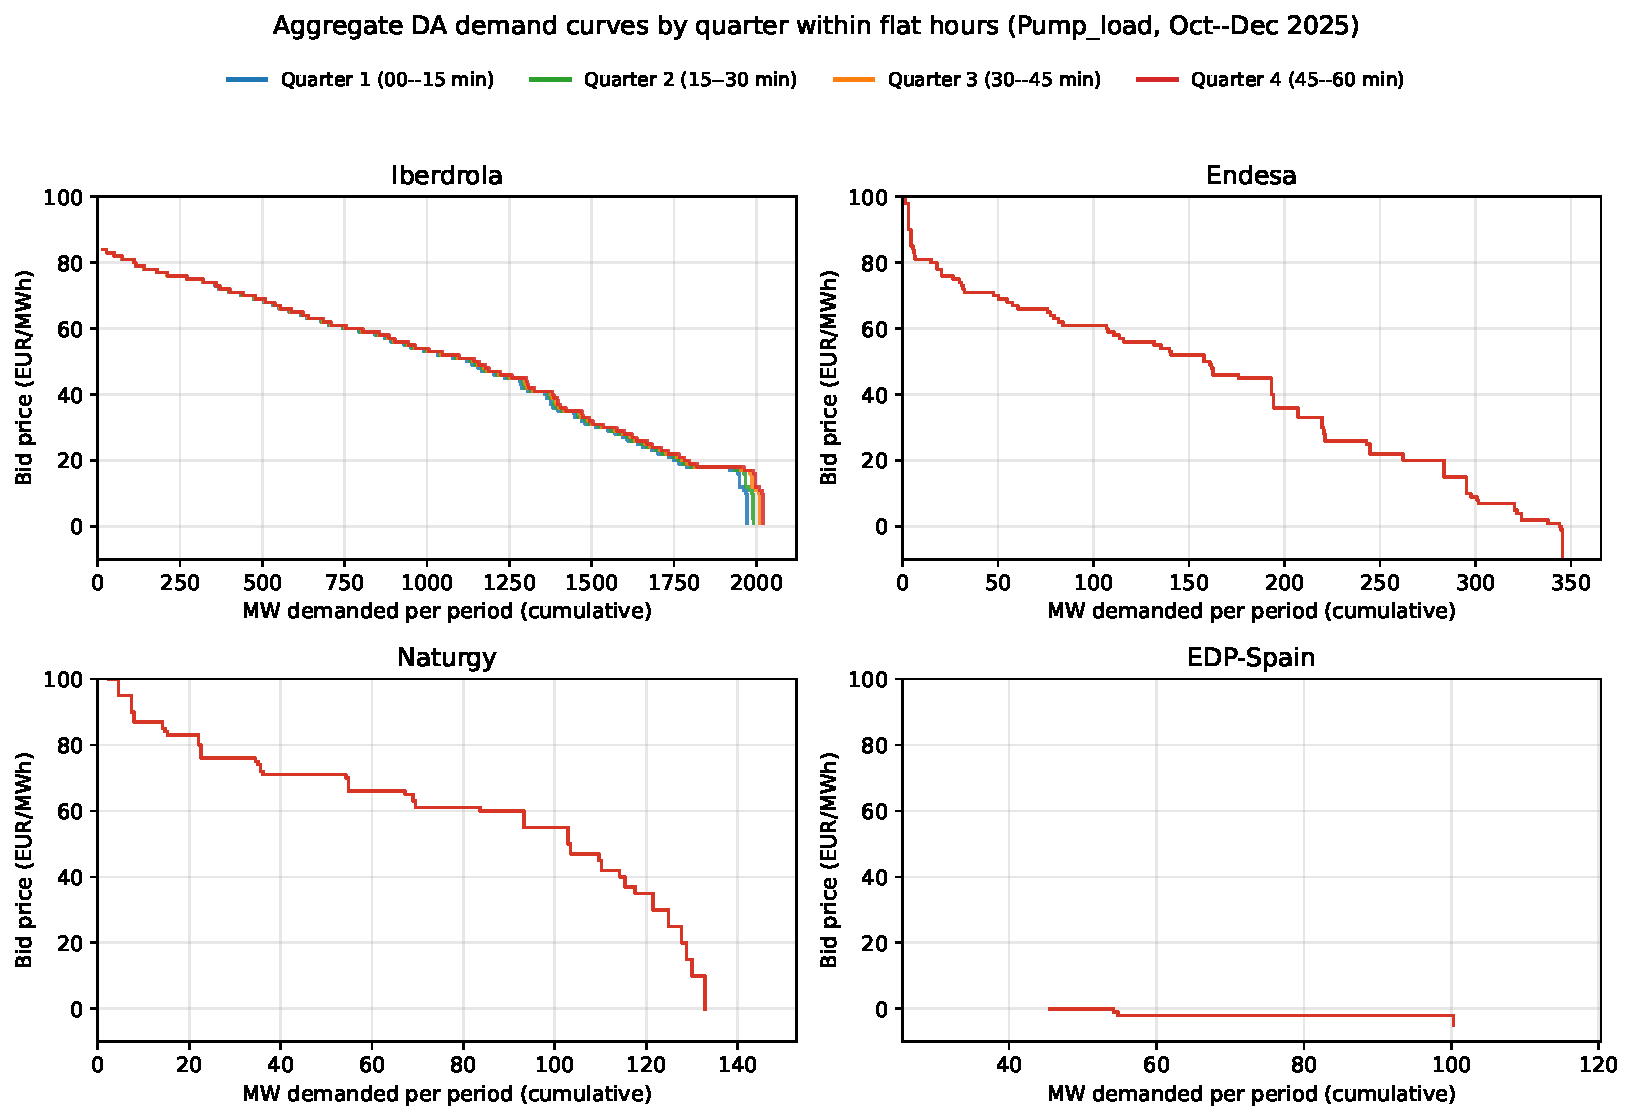
\includegraphics[width=\textwidth]{fig_per_firm_demand_curves_quarters_pump_load_flat.pdf}
\caption{DA, flat hours}
\end{subfigure}
\caption{Aggregate DA demand curves by quarter, pump-storage charge bids, Oct--Dec 2025. The IDA-side analogue is similar and is not reproduced.}
\end{figure}


% =====================================================================
\subsection{Results: per-curve functionals, and the pairwise $D_w$ diagnostic}\label{sec:prov:dw_tables}

\noindent The results below quantify what the bid-curve figures in \S\ref{sec:prov:bid_graphs} show visually: first the Family-1 per-curve functionals ($\sigma_p$, $N_{\text{eff}}$, defined in \S\ref{sec:prov:per_curve_def}), then the Family-2 pairwise $D_w$ diagnostic (\S\ref{sec:prov:dw_decomp_def}).

\paragraph{Per-curve functionals: price spread and effective tranche count.}
Table~\ref{tab:per_curve_metrics} and Figure~\ref{fig:per_curve_metrics} report $\sigma_p$ and $N_{\text{eff}}$ averaged over (unit, date, period) day-ahead sell-bid curves, by tech, hour-class and regime --- the cross-regime reading is a comparison of per-curve \emph{values}, with no differencing of curves.

\begin{table}[H]
\centering\footnotesize
\caption{\textbf{Per-curve bid-shape metrics by tech, hour-class and regime} (DA sell bids, in-band $|p-\text{MCP}|\le 50$, mean over (unit, date, period) curves). $\sigma_p$ = MW-weighted price spread (EUR/MWh); $N_{\text{eff}}$ = effective in-band tranche count. $452{,}762$ in-band curves.}
\label{tab:per_curve_metrics}
\setlength{\tabcolsep}{4pt}
\begin{tabular}{l l r r r r r r r r r r }
\toprule
 & & \multicolumn{2}{c}{3-sess} & \multicolumn{2}{c}{ISP15-win} & \multicolumn{2}{c}{DA60/ID15 pre} & \multicolumn{2}{c}{DA60/ID15 post} & \multicolumn{2}{c}{DA15/ID15} \\
Tech & Hour & $\sigma_p$ & $N_{\text{eff}}$ & $\sigma_p$ & $N_{\text{eff}}$ & $\sigma_p$ & $N_{\text{eff}}$ & $\sigma_p$ & $N_{\text{eff}}$ & $\sigma_p$ & $N_{\text{eff}}$ \\
\midrule
CCGT & Critical & 36.1 & 3.3 & 32.0 & 4.2 & 29.2 & 3.1 & 24.5 & 3.1 & 25.5 & 3.4 \\
CCGT & Flat & 27.5 & 2.5 & 45.2 & 2.7 & 17.1 & 2.3 & 20.2 & 2.6 & 18.4 & 2.2 \\
\addlinespace
Hydro & Critical & 17.5 & 4.0 & 16.3 & 4.0 & 13.1 & 3.5 & 15.5 & 3.5 & 18.3 & 3.9 \\
Hydro & Flat & 17.6 & 4.0 & 18.5 & 3.8 & 12.6 & 3.5 & 16.0 & 3.5 & 17.0 & 3.9 \\
\addlinespace
Hydro pump & Critical & 3.6 & 2.5 & 3.8 & 2.5 & 2.6 & 2.3 & 3.9 & 2.8 & 4.3 & 3.5 \\
Hydro pump & Flat & 2.1 & 2.6 & 3.9 & 2.9 & 2.4 & 2.3 & 2.6 & 2.4 & 2.9 & 4.2 \\
\addlinespace
\bottomrule
\end{tabular}
\end{table}

\begin{figure}[H]
\centering
\includegraphics[width=0.95\textwidth]{../../figures/working/per_curve_metrics.pdf}
\caption{\textbf{Per-curve bid-shape metrics across regimes} (DA, in-band). Left: price spread $\sigma_p$; right: effective tranche count $N_{\text{eff}}$. Each line is a (tech, hour-class) cell; solid = critical hours, dashed = flat. Hydro carries the widest price spread (water-value bidding spans a range); CCGT's $\sigma_p$ is consistently larger in critical than flat hours --- the strategic signal. $N_{\text{eff}}$ rises across the reform sequence for all three price-setting techs.}
\label{fig:per_curve_metrics}
\end{figure}

\paragraph{The pairwise $D_w$ diagnostic (Family 2).} The $D_w$ / $\Delta p$ / $\Delta q$ statistics below are the Family-2 \emph{pairwise} construction (\S\ref{sec:prov:dw_decomp_def}) --- they compare a unit's four within-hour quarter curves to each other. They remain a useful within-hour-shaping diagnostic, but the per-curve functionals above are the primary descriptive object. We report (i) the per-cell binary flag $D_w > 0$ across techs and firms (operational vs strategic decomposition, IDA pre/post-blackout) and (ii) the $\Delta p / \Delta q$ channel-shares and intensity tables.

\paragraph{DA Oct--Dec 2025: operational vs strategic decomposition by (tech, firm).}\label{sec:prov:operational_strategic}
\textit{Reading} (\textbf{mixed}). The original main-paper framing reported a critical--flat asymmetry with the interpretation ``only Naturgy CCGT shows the strategic signature''. The IDA pre/post-blackout analysis (below) and the multitech within-hour shaping table (at the end of this subsection) complicate this: GN's CCGT $D_w$ activity is real and large, IB hydro and pump-storage are also highly active, and under reforzada all four firms show the IDA-side strategic signature, not just Naturgy.

\begin{table}[H]
\centering\footnotesize
\caption{\textbf{DA Oct--Dec 2025 critical--flat asymmetry, by (channel, technology, firm).} Percentage of (firm, unit, date, hour) cells with $D_w > 0$. \emph{Channel}: Strategic = exploitation of within-hour granularity near clearing; Operational = forecast/load-shape updates; Mechanical = smooth pump-storage charge. Compare: IDA in Table~\ref{tab:ida_pre_post}, multitech in Table~\ref{tab:within_hour_shaping}.}
\label{tab:prov:operational_strategic_asym}
\setlength{\tabcolsep}{6pt}
\begin{tabular}{l l l r r r}
\toprule
Channel & Tech & Firm & \% crit & \% flat & Crit$-$Flat (pp) \\
\midrule
Strategic & CCGT & GN & 24.5 & 0.0 & $+24.5$ \\
Strategic & CCGT & IB & 5.8 & 3.9 & $+1.9$ \\
\addlinespace
Operational & Wind & IB & 97.2 & 97.3 & $-0.1$ \\
Operational & Wind & GN & 92.7 & 92.6 & $+0.1$ \\
Operational & Wind & HC & 93.7 & 93.8 & $-0.1$ \\
Operational & Solar PV & GN & 15.9 & 0.0 & $+15.9$ \\
Operational & Retailer & GE & 76.5 & 76.3 & $+0.2$ \\
Operational & Retailer & IB & 40.9 & 40.2 & $+0.7$ \\
Operational & Direct\_consumer & IB & 96.0 & 95.3 & $+0.7$ \\
\addlinespace
Mechanical & Pump\_load & IB & 3.2 & 5.5 & $-2.3$ \\
Mechanical & Pump\_load & GE & 0.0 & 0.0 & $0.0$ \\
Mechanical & Hydro\_pump & IB & 0.4 & 0.0 & $+0.4$ \\
Mechanical & Hydro\_pump & GE & 0.0 & 0.0 & $0.0$ \\
\bottomrule
\end{tabular}
\end{table}

\paragraph{IDA pre/post-blackout near-clearing dissimilarity.}\label{sec:prov:ida_pre_post}
For each (firm, unit, date, hour) CCGT IDA cell, Epanechnikov-weighted within-hour quarter dissimilarity $D_w$ ($h = 50$ EUR/MWh, centred on hour-mean IDA clearing price). Pre-blackout: 2025-03-19 $\to$ 2025-04-27. Post-blackout: 2025-04-28 $\to$ 2025-09-30 (reforzada). Hypothesis: REE post-clearing intervention should remove the leverage on clearing price, so pre $>$ post.

\begin{table}[H]
\centering
\caption{\textbf{IDA quarter-dissimilarity, pre vs post-blackout, CCGT.} Percentage of (firm, unit, date, hour) cells with $D_w > 0$ (i.e., quarters differ within the Epanechnikov band, $h = 50$~EUR/MWh, around hour-mean IDA clearing price). \emph{Pre-blackout}: 2025-03-19 $\to$ 2025-04-27 (40 days, MTU15-IDA active, reforzada-free). \emph{Post-blackout}: 2025-04-28 $\to$ 2025-09-30 (155 days, reforzada active).}
\label{tab:ida_pre_post}
\begin{tabular}{l r r r r r r}
\toprule
& \multicolumn{3}{c}{Pre-blackout} & \multicolumn{3}{c}{Post-blackout} \\
\cmidrule(lr){2-4}\cmidrule(lr){5-7}
Firm & Critical & Flat & Crit$-$Flat & Critical & Flat & Crit$-$Flat \\
\midrule
IB & 9.6 & 7.0 & $+2.6$ & 20.3 & 6.2 & $+14.1$ \\
GE & 14.1 & 10.0 & $+4.1$ & 43.8 & 33.2 & $+10.6$ \\
GN & 30.5 & 9.2 & $\mathbf{+21.3}$ & 53.8 & 37.9 & $+15.9$ \\
HC & 27.9 & 20.7 & $+7.2$ & 34.2 & 21.2 & $+13.0$ \\
\bottomrule
\end{tabular}
\end{table}

\textit{Reading} (\textbf{mixed}). (i) Pre: only GN shows clean asymmetry ($+21$pp). (ii) Post: all four firms show $+11$ to $+16$pp gap. (iii) Pre $>$ post rejected for every firm; rates roughly double. (iv) Flat-hour rates post-blackout 6--38\% (reforzada-driven operational adjustments); the critical-flat asymmetry is the \emph{lower bound} on strategic activity.

\textit{Verdict} (\textbf{mixed}). The directional prediction (pre $>$ post) is rejected, but the critical-vs-flat asymmetry survives and broadens to all four firms. Reading: pay-as-bid RT2 + intra-tech competition $\Rightarrow$ the strategic-bidding mechanism is essentially unchanged from pre-reforzada. The relevant new lever is geographic (\S\ref{sec:prov:geo}).

% \paragraph{Source data.} \code{scripts/analysis/bid/quarter_dissimilarity_ida.py}; outputs at \code{results/regressions/bid/quarter_dissimilarity_ida/}.


% =====================================================================
\paragraph{$\Delta p$ / $\Delta q$ channel shares (CCGT, DA Oct--Dec 2025).}\label{sec:prov:dw_decomp_results}
\emph{Methodology and decomposition: see \S\ref{sec:prov:dw_decomp_def}. Outcomes below are the share of cells where each channel is active and the median value conditional on active. Caveat: raw $\Delta q$ in MWh is coarse on its own --- see the $\Delta q$ caveat in \S\ref{sec:prov:dw_decomp_def}.}

\begin{table}[H]
\centering
\caption{\textbf{DA Oct--Dec 2025, CCGT.} \textbf{Outcomes:} \emph{$\Delta p$-active (\%)} = \% of cells with $\Delta p_{ij} > 0$ for at least one within-hour pair (price channel is active); \emph{$\Delta q$-active (\%)} = same for the quantity channel; \emph{med $\Delta p$} = median pair-wise $\Delta p$ in EUR/MWh over the cells where the price channel is active; \emph{med $\Delta q$} = same in MWh for the quantity channel. Strategic band $|p - c| \le 50$ EUR/MWh. Pair-wise statistics aggregated to cell via max across the 6 quarter-pairs.}
\label{tab:dw_decomp}
\begin{tabular}{l l r r r r r}
\toprule
Firm & Hour & $n$ cells & $\Delta p$-active (\%) & $\Delta q$-active (\%) & med $\Delta p$ (EUR/MWh) & med $\Delta q$ (MWh) \\
\midrule
\textbf{GN} & critical & 14\,930 & \textbf{0.01} & \textbf{18.4} & 3.4 & 147 \\
GN & flat & 4\,065 & 0.00 & 0.00 & --- & --- \\
\addlinespace
GE & critical & 5\,195 & 1.56 & 0.33 & 4.6 & 364 \\
GE & flat & 1\,413 & 0.00 & 0.00 & --- & --- \\
\addlinespace
IB & critical & 7\,831 & 0.10 & 1.94 & 3.9 & 70 \\
IB & flat & 2\,139 & 0.89 & 1.03 & 3.1 & 11 \\
\addlinespace
HC & critical & 2\,013 & 0.00 & 0.05 & --- & 60 \\
HC & flat & 549 & 0.00 & 0.00 & --- & --- \\
\bottomrule
\end{tabular}
\end{table}

\textit{Reading} (\textbf{supportive}). (i) GN: 18.4\% $\Delta q$-active, 0.01\% $\Delta p$-active --- shaping is quantity-only. (ii) Flat hours: 0\% on both channels for GN/GE/HC. (iii) GE has the opposite mix (1.56\% $\Delta p$ vs 0.33\% $\Delta q$), both small. (iv) IB/HC: negligible. \emph{Caveat:} the raw $\Delta q$ medians (e.g.\ GN crit 147 MWh, GE crit 364 MWh) should be read alongside firm-level mean band-mass to interpret the proportional size --- see setup section's caveat on $\Delta q$.

\textit{Verdict} (\textbf{supportive}). GN fixes the price ladder near the cap and re-allocates quantity across the 4 quarters: the Cournot version of price-raising. Unit tests (identical-curves $\to$ 0/0; same-price-diff-mass $\to$ 0/$+$; same-mass-diff-price $\to$ $+$/0) confirm the decomposition is mathematically correct.
% Unit tests: scripts/analysis/bid/w1_decomposition.py


% =====================================================================
\paragraph{$D_w$ distributions across firms, technologies, and regimes.}\label{sec:prov:dw_distributions}
The next table summarises the $D_w$ distribution by sample: the mass at $D_w = 0$ (no within-hour quarter variation in the band) and, conditional on $D_w > 0$, the median value.

\begin{table}[H]
\centering\scriptsize
\caption{\textbf{CCGT mass at $D_w = 0$ and conditional median $D_w$, by sample.} \textbf{Outcome:} share of (firm, unit, date, hour) cells with $D_w = 0$ (no within-hour quarter variation in the Epanechnikov band $|p-c| \le h$ around clearing) and, conditional on $D_w > 0$, the median $D_w$ value (units: EUR --- $D_w$ multiplies a quantity in MWh by a price in EUR/MWh, so it has dimension EUR; see \S\ref{sec:prov:dw_decomp}). Three samples: DA Oct--Dec 2025 (post-MTU15-DA), IDA pre-blackout (2025-03-19 to 2025-04-27), IDA post-blackout (2025-04-28 to 2025-09-30).}
\label{tab:dw_mass_median}
\setlength{\tabcolsep}{4pt}
\begin{tabular}{l l r r r r}
\toprule
Sample & Firm & \% crit cells $D_w {=} 0$ & \% flat cells $D_w {=} 0$ & med $D_w$ crit (EUR) & med $D_w$ flat (EUR) \\
\midrule
\multirow{4}{*}{DA Oct--Dec 2025} & IB & 98 & 98 & 415 & 154 \\
 & GE & 98 & 100 & 1\,333 & --- \\
 & GN & 77 & 100 & 5\,167 & 2\,287 \\
 & HC & 100 & 100 & --- & --- \\
\midrule
\multirow{4}{*}{IDA pre-blackout} & IB & 90 & 93 & 142 & 6 \\
 & GE & 86 & 90 & 503 & 108 \\
 & GN & 70 & 91 & 504 & 242 \\
 & HC & 72 & 79 & 735 & 761 \\
\midrule
\multirow{4}{*}{IDA post-blackout}& IB & 80 & 94 & 229 & 342 \\
 & GE & 56 & 67 & 498 & 165 \\
 & GN & 46 & 62 & 836 & 322 \\
 & HC & 66 & 79 & 835 & 674 \\
\bottomrule
\end{tabular}
\end{table}

\textit{Reading} (\textbf{supportive}). (i) DA mass-at-zero $\approx$ identical critical vs flat for every firm except GN (77\% vs 100\%). (ii) IDA: post-blackout shifts mass-at-zero down for every firm; \%crit-at-0 $<$ \%flat-at-0 in every (firm, regime). (iii) Conditional median $D_w$ in critical hours $\approx$ 2--3$\times$ flat for GN, GE on IDA. (iv) Strategic signature (mass-asymmetry critical $<$ flat) appears only in CCGT and Solar~PV; operational categories overlap.

\paragraph{Within-hour strategic shaping by (tech, firm), DA15/ID15 critical hours.} The partial-acceptance frame in \S\ref{sec:prov:pricesetter_da} ranks who clears at MCP. The bid-shape frame here asks who actively shapes within-hour bids across the 4 quarters, regardless of whether their bid lands at MCP. We compute $\Delta p_{\max}$ and $\Delta q_{\max}$ (kernel band $\pm 50$ around MCP). A unit is ``$\Delta p$-active'' in an hour-cell iff $\Delta p_{\max} > 0$ (similarly $\Delta q$-active).
% Multitech analysis: scripts/analysis/bid/w1_decomposition_top_units.py

\begin{table}[H]
\centering\scriptsize
\caption{\textbf{Within-hour strategic shaping by tech and firm, DA15/ID15 critical hours.} \%-act = share of hour-cells with $\Delta_{\max} > 0$; med-$\Delta$ conditional on active.}
\label{tab:within_hour_shaping}
\setlength{\tabcolsep}{3pt}
\begin{tabular}{@{}l l r r r r r r@{}}
\toprule
Tech & Firm (top units) & $n$ units & $n$ cells & \% $\Delta p$-act & \% $\Delta q$-act & med $\Delta p$ & med $\Delta q$ \\
 & & & & & & (EUR/MWh) & (MWh) \\
\midrule
CCGT & \textbf{IB} & 4 & 1{,}935 & \textbf{68.3} & 74.5 & 0.23 & 382 \\
CCGT & \textbf{GN} & 13 & 5{,}906 & \textbf{32.6} & 52.9 & \textbf{4.14} & 211 \\
CCGT & GE & 4 & 1{,}570 & 8.6 & 77.5 & 3.48 & 371 \\
\midrule
Wind & \textbf{GST} & 2 & 1{,}076 & \textbf{96.3} & \textbf{98.9} & 5.06 & 19 \\
Wind & IB (IBEVD11) & 1 & 250 & 23.6 & 27.2 & 0.34 & \textbf{1{,}291} \\
Wind & HC (EDP) & 3 & 1{,}638 & 9.3 & 17.2 & 0.65 & 238 \\
Wind & AXPO, NEXUS & 3 & 1{,}013 & 0.0 & 13--16 & --- & 1--13 \\
\midrule
Hydro & \textbf{IB} & 3 & 1{,}638 & \textbf{73.8} & 79.4 & 4.02 & 448 \\
Hydro & GE (GDLQ) & 1 & 402 & 22.4 & 23.9 & 0.16 & 73 \\
\midrule
Pump-st. & \textbf{IB (MUEL)} & 1 & 540 & \textbf{88.0} & 88.9 & 1.90 & \textbf{1{,}221} \\
Pump-st. & \textbf{GE (MLTG)} & 1 & 418 & \textbf{86.1} & 91.6 & 3.44 & 195 \\
\bottomrule
\end{tabular}
\end{table}

\textit{Reading} (\textbf{supportive}). GN ranks at 0\% of CCGT \emph{price-setting} (their bids are too high to land at MCP, see \S\ref{sec:prov:pricesetter_da}) but here actively shapes within-hour bids in $33\%$ of critical hours with the largest median $\Delta p$ of any CCGT firm. Iberdrola is the dominant strategic actor across CCGT (68\%), hydro (74\%), and pump-storage (88\%). Wind aggregators split sharply: Gesternova (independent) ladder-bids across quarters (96\% $\Delta p$-active); IBEVD11 (Iberdrola, volume giant) shifts quantities but not prices --- forecast-driven, not strategic; AXPO and NEXUS bid identically across all 4 quarters. The MTU15-DA reform is exploited by specific firm-unit combinations, not uniformly.


% =====================================================================
\subsection{Functional PCA of bid-curve shape changes across regimes}\label{sec:prov:fpca}
% =====================================================================

\paragraph{Motivation and method.} The two per-curve functionals of \S\ref{sec:prov:per_curve_def} ($\sigma_p$, $N_{\text{eff}}$) fix the shape coordinate in advance. Functional PCA (fPCA) is the data-driven member of the same Family~1: it still maps each single curve to scalars, but lets the data choose the modes. It treats each per-(unit, date, period) sell bid stack as a functional observation --- the inverse supply curve $f_i(q) = S_i^{-1}(q)$ on cumulative-MW quantiles $q \in [0,1]$ --- and extracts orthogonal modes of shape variation. With sample mean $\bar f$, fPCA finds an orthonormal basis $\{\phi_k\}$ with uncorrelated scores
\[
\xi_{ik} \;=\; \langle f_i - \bar f,\, \phi_k\rangle_{L^2} \;=\; \int_0^1 \left[f_i(q) - \bar f(q)\right] \phi_k(q)\, dq,
\]
and the Karhunen-Lo\`eve expansion $f_i(q) = \bar f(q) + \sum_k \xi_{ik}\, \phi_k(q)$ replaces each curve by $K$ scalar scores. PC1 typically captures a level shift, PC2 a cheap-vs-scarcity tilt, higher PCs finer shape. Quantile space is scale-normalised across units of any size; we pool per tech (a single pooled PCA would burn PC1 on cross-tech mean differences). To keep PC1 orthogonal to the calendar cycle we deseasonalise functionally before PCA: at each quantile grid point $q$, subtract the seasonality-only fit of the FWL spec of \S\ref{sec:bid_internal:calendar_discipline}, $f_i^{\text{SA}}(q) = f_i(q) - \widehat{\text{seas}}_i(q)$.

\textbf{Explained variance.} The first PC captures most of the variation:
\begin{center}\scriptsize
\begin{tabular}{l r r r r r r}
\toprule
Tech & PC1 & PC2 & PC3 & PC4 & PC5 & Cumulative top-5 \\
\midrule
CCGT & 0.86 & 0.08 & 0.03 & 0.01 & 0.01 & 0.98 \\
Hydro & 0.91 & 0.06 & 0.01 & 0.01 & 0.00 & 0.99 \\
Hydro pump & 0.89 & 0.07 & 0.01 & 0.01 & 0.00 & 0.99 \\
Nuclear & 0.62 & 0.17 & 0.08 & 0.04 & 0.02 & 0.93 \\
Wind & 0.78 & 0.10 & 0.04 & 0.02 & 0.01 & 0.96 \\
Solar PV & 0.89 & 0.06 & 0.02 & 0.01 & 0.00 & 0.98 \\
Cogen & 0.62 & 0.19 & 0.12 & 0.03 & 0.02 & 0.97 \\
\bottomrule
\end{tabular}
\end{center}

\paragraph{Score regression: pairwise reform-window design.} Each reform is isolated by restricting the sample to its immediate before/after windows (ISP15: 3-sess $\to$ ISP15-win; MTU15-IDA: ISP15-win $\to$ DA60/ID15 pre-blk; MTU15-DA: DA60/ID15 post-blk $\to$ DA15/ID15). For each (tech, firm) and reform we run, separately per PC $k$, on the SA scores:
\begin{align*}
\xi^{\text{SA}}_{i,k} = \alpha &+ \beta_{0,k}\, \mathds{1}[\text{post}_i]
 + \!\sum_{h \in \{\text{Flat}, \text{Mid}\}}\! \beta_{h,k}\, \mathds{1}[\text{post}_i]\,\mathds{1}[\text{hour}_i = h]
 + \gamma_k\, X_i + \varepsilon_{i,k},
\end{align*}
where $X_i$ collects calendar-month, hour-of-day, and within-hour quarter FE. The post-effect is $\beta_{0,k}$ on Critical hours, $\beta_{0,k} + \beta_{h,k}$ on Flat/Midday. Table~\ref{tab:fpca_pc123_all} reports each pre-post PC change projected back onto the curve domain via $\widehat\beta_k \cdot \phi_k$ (EUR/MWh, summed across quantiles).

\begin{table}[H]
\centering\scriptsize
\caption{\textbf{Pairwise PC1, PC2, PC3 coefficients across all three reforms (functional-SA), critical hours.} Cells in EUR/MWh on the curve domain (post coefficient projected via $\beta_k \phi_k(q)$, summed). The MTU15-IDA panel uses a 40-day post window. RES techs (Wind, Solar PV, Cogen, Solar Thermal) are aggregated per firm into ``OTH'' (RES has too many small distributed units for per-firm fPCA).}
\label{tab:fpca_pc123_all}
\setlength{\tabcolsep}{4pt}
% Merged fPCA PC1/PC2/PC3 tables for all three reforms (functional-SA scores).
\begin{tabular}{@{}l l r r r r r r r r r @{}}
\toprule
 & & \multicolumn{3}{c}{\textbf{ISP15}} & \multicolumn{3}{c}{\textbf{MTU15-IDA}} & \multicolumn{3}{c}{\textbf{MTU15-DA}} \\
\cmidrule(lr){3-5}\cmidrule(lr){6-8}\cmidrule(lr){9-11}
Tech & Firm & PC1 & PC2 & PC3 & PC1 & PC2 & PC3 & PC1 & PC2 & PC3 \\
\midrule
CCGT & GE & +3459 & +2042 & +903 & +2560 & -260 & -1022 & -15018 & +879 & -183 \\
 & GN & +315 & +109 & +32 & -206 & +107 & -38 & +862 & -736 & +30 \\
 & HC & -1573 & +240 & +175 & -611 & +9 & -323 & +2480 & -270 & +166 \\
 & IB & -1558 & -60 & -253 & +16 & -248 & +233 & +1849 & -583 & -218 \\
 & AXPO & -1567 & -188 & -139 & +189 & +12 & +60 & +1217 & -609 & -116 \\
 & REP & -1368 & +44 & -377 & -258 & -383 & +164 & +1451 & -630 & -163 \\
 & OTH & -1349 & -61 & -133 & +45 & -122 & -90 & +2183 & -485 & -78 \\
\addlinespace
Hydro & GE & +134 & +124 & +0 & -750 & -41 & -22 & -384 & -6 & +5 \\
 & GN & +351 & +95 & -8 & +252 & +58 & +31 & -173 & -59 & -42 \\
 & HC & +519 & -331 & +29 & -243 & -44 & +84 & +305 & -264 & -137 \\
 & IB & +1047 & -134 & -108 & -269 & -91 & +112 & -188 & +25 & +6 \\
 & REP & -10 & -47 & -20 & -322 & +95 & +77 & +55 & -39 & -89 \\
 & OTH & -374 & +100 & -8 & +85 & +30 & +12 & -702 & -18 & +3 \\
\addlinespace
Hydro pump & GE & -280 & +76 & -7 & -359 & -11 & +0 & -305 & -16 & +0 \\
 & GN & +333 & +77 & -9 & -112 & -83 & +105 & +1272 & -19 & +3 \\
 & IB & -59 & -108 & -41 & -471 & -132 & +68 & -57 & -44 & -29 \\
 & REP & -145 & +1 & +35 & -366 & -143 & +89 & -380 & +145 & -68 \\
\addlinespace
Nuclear & GE & -1076 & -361 & +64 & +0 & +512 & +238 & +1681 & -767 & -1498 \\
 & GN & -632 & +152 & +79 & -65 & +396 & +140 & +2132 & -1322 & +380 \\
 & IB & -842 & +87 & -13 & +62 & +393 & +188 & +763 & -1666 & -516 \\
\addlinespace
Wind & OTH & -50 & -9 & +4 & +17 & -1 & +1 & +8 & +17 & -12 \\
\addlinespace
Solar PV & OTH & +474 & +39 & +11 & +416 & -78 & +33 & +1599 & +102 & +6 \\
\addlinespace
Solar Thermal & OTH & +68 & +11 & +5 & -23 & +26 & -26 & -42 & +13 & +14 \\
\addlinespace
Cogen & OTH & -26 & -9 & +11 & +5 & -21 & +14 & +121 & +182 & -136 \\
\bottomrule
\end{tabular}

\end{table}

\paragraph{Reading the fPCA evidence.}
\begin{itemize}\setlength{\itemsep}{2pt}
\item \textbf{Headline level shifts.} GE-CCGT moves opposite to GN/IB/HC under every reform: up under ISP15 ($+3{,}459$ Critical, PC1) and MTU15-IDA, sharply down under MTU15-DA ($-15{,}018$ Critical, the largest single SA coefficient); IB-CCGT $+1{,}849$, HC-CCGT $+2{,}480$, GN-CCGT $+862$ under MTU15-DA.
\item \textbf{PC2/PC3 carry weight where the reform changes tilt, not level.} Nuclear under MTU15-IDA has PC1 near zero but PC2 $+393$ to $+512$ across GE/GN/IB --- a within-curve tilt PC1 misses. CCGT under MTU15-DA has positive PC1 but negative PC2 ($-270$ to $-879$) for five of seven firms: cheap-MW tranches repriced up more than the scarcity tail.
\item \textbf{Identification caveat.} MTU15-DA and reforzada are both active in the MTU15-DA post-window; the coefficient is the joint shift. Only the 40-day MTU15-IDA pairwise is a clean single-reform read. A year-fold placebo (2022/2023 calendar windows) flags the GE-CCGT ISP15 raw shift as seasonal, while the CCGT IB/HC/GE MTU15-DA critical-hour pattern survives both controls.
\end{itemize}

% =====================================================================
\section{Continuous-intraday repositioning per technology}\label{sec:prov:ci_per_tech}
% =====================================================================

\textbf{Why this matters.} The system-cost evidence in \S\ref{sec:prov:full_cascade} documents the redistribution of expenditure between TR (real-time technical restrictions) and Fase~I (pre-IDA pay-as-bid redispatch). What the cascade view does not show is the bidding-side mechanism through which the cost reallocation materialises. The hypothesis is that finer-grained intraday clearing absorbs within-hour scarcity that previously spilled into real-time correction; if true, this should be visible in the volume of repositioning that technologies do in the post-IDA continuous market (XBID). We characterise per-technology continuous-intraday (CI) activity across the reform regimes.

\textbf{Variable.} Each XBID matched trade pairs a buyer unit and a seller unit (with a contract quantity in MW for a delivery period of the relevant MTU length). For each (delivery date, technology) we sum the MWh of CI trades on the sell side (the technology of the seller unit) and on the buy side (the technology of the buyer unit), then average per day within each regime. The \emph{gross} CI activity per tech is the sum of sells and buys; the \emph{net} CI position is sells minus buys. \textbf{Sources}: XBID matched-trade panel and unit-to-technology bridge.
% trades_all.parquet (XBID matches) joined to lista_unidades.csv on seller_unit/buyer_unit.

\begin{table}[H]
\centering
\caption{\textbf{Gross continuous-intraday activity by technology and regime, GWh/day.} Sum of sell-side and buy-side MWh per (delivery date, technology), averaged per day per regime. Captures total CI repositioning by tech.}
% Source: results/regressions/bid/ci_position_adjustments/per_tech_gross_gwh_day.tex
\label{tab:ci_gross_per_tech}
\setlength{\tabcolsep}{4pt}
\scriptsize
\begin{tabular}{l r r r r r r }
\toprule
 & \textbf{pre-IDA} & \textbf{3-sess} & \textbf{ISP15-win} & \textbf{MTU15 pre-blk} & \textbf{MTU15 post-blk} & \textbf{DA15/ID15} \\
\midrule
CCGT & 1.3 & 3.9 & 4.4 & 1.9 & 2.4 & 3.7 \\
Nuclear & 2.4 & 3.8 & 3.5 & 1.3 & 3.8 & 4.1 \\
Hydro & 3.3 & 4.2 & 4.5 & 2.6 & 2.4 & 3.2 \\
Hydro pump & 1.6 & 2.2 & 2.1 & 1.5 & 1.1 & 1.0 \\
Wind & 5.5 & 6.5 & 5.1 & 3.5 & 3.6 & 7.5 \\
Solar PV & 3.7 & 3.5 & 2.1 & 2.2 & 3.0 & 3.5 \\
Solar Thermal & 0.4 & 0.7 & 0.5 & 0.6 & 0.6 & 0.3 \\
Biomass / RE thermal & 0.4 & 0.6 & 0.5 & 0.5 & 0.4 & 0.4 \\
Thermal non-RE & 0.2 & 0.3 & 0.4 & 0.4 & 0.3 & 0.3 \\
Battery / storage & 0.0 & 0.0 & 0.0 & -- & 0.1 & 0.1 \\
Cogen & -- & -- & -- & -- & -- & -- \\
\bottomrule
\end{tabular}

\end{table}

\begin{table}[H]
\centering
\caption{\textbf{Net continuous-intraday position by technology and regime, GWh/day.} Sells $-$ buys per (delivery date, technology). Positive values $=$ net seller (technology adds output via CI); negative $=$ net buyer (technology reduces output via CI).}
% Source: results/regressions/bid/ci_position_adjustments/per_tech_net_gwh_day.tex
\label{tab:ci_net_per_tech}
\setlength{\tabcolsep}{4pt}
\scriptsize
\begin{tabular}{l r r r r r r }
\toprule
 & \textbf{pre-IDA} & \textbf{3-sess} & \textbf{ISP15-win} & \textbf{MTU15 pre-blk} & \textbf{MTU15 post-blk} & \textbf{DA15/ID15} \\
\midrule
CCGT & +0.8 & +2.5 & +2.5 & +1.3 & +1.6 & +2.2 \\
Nuclear & $-$1.2 & $-$1.0 & $-$1.7 & +0.3 & $-$2.9 & $-$0.2 \\
Hydro & +0.7 & +0.9 & +1.1 & +0.2 & +0.2 & +0.6 \\
Hydro pump & +0.1 & $-$0.0 & +0.1 & $-$0.0 & +0.1 & $-$0.1 \\
Wind & $-$0.1 & $-$0.5 & $-$0.4 & +0.5 & +0.2 & $-$1.2 \\
Solar PV & +0.4 & $-$0.3 & $-$0.1 & $-$0.3 & $-$0.3 & +0.1 \\
Solar Thermal & $-$0.1 & $-$0.1 & $-$0.1 & +0.1 & $-$0.2 & $-$0.1 \\
Biomass / RE thermal & $-$0.1 & $-$0.3 & $-$0.2 & $-$0.2 & $-$0.2 & $-$0.2 \\
Thermal non-RE & $-$0.0 & $-$0.0 & $-$0.1 & +0.0 & $-$0.1 & $-$0.1 \\
Battery / storage & +0.0 & +0.0 & $-$0.0 & -- & +0.0 & +0.0 \\
Cogen & -- & -- & -- & -- & -- & -- \\
\bottomrule
\end{tabular}

\end{table}

\textit{Reading.}
\begin{itemize}\setlength{\itemsep}{2pt}
\item \textbf{System-wide gross CI activity falls during MTU15-IDA, then recovers under MTU15-DA.} The sum across techs of the gross CI volume (sells side) drops from $\sim$20 GWh/day pre-reforms to $\sim$13 GWh/day during the MTU15-IDA-only window (Mar--Sep 2025) and recovers to $\sim$19 GWh/day after MTU15-DA. The drop is consistent with the auction-based IDA15 absorbing intra-hour scarcity that previously fell to XBID. The recovery is consistent with the finer-grained DA15 producing more per-quarter mismatch that XBID is structurally well placed to close.

\item \textbf{Wind doubles its CI activity under MTU15-DA.} Wind onshore gross CI volume goes from 3.5--3.6 GWh/day in the MTU15-IDA-only window to 7.5 GWh/day under MTU15-DA --- the largest tech-specific increase in the table. Forecast-error correction at quarter-hour resolution is the natural reading: granular DA + granular CI lets wind units re-balance against their forecast at each ISP, where the pre-MTU15-DA infrastructure forced them to bundle into hourly settlement cells.

\item \textbf{CCGTs are systematic net SELLERS in CI in every regime.} The net-position column (Table~\ref{tab:ci_net_per_tech}) shows CCGT at $+0.8$ to $+2.5$ GWh/day across regimes; the firm adds output via the continuous market in the typical day. This is consistent with the headline ``DA-stay-out, re-enter via post-clearing channels'' narrative in \S\ref{sec:prov:q1_drop}--\S\ref{sec:prov:geo}: CCGTs that did not clear DA can rejoin via XBID (or via Fase~I redispatch), and the bid-side observable for the XBID side is the net-positive CI sell flow.

\item \textbf{Nuclear is the systematic net BUYER, especially in the post-blackout window.} Nuclear net-buys $-1.7$ to $-2.9$ GWh/day in the operational-reforzada window (a position reduction relative to DA-clearing). The mechanism is the RES-curtailment $+$ system-rebalancing regime that forced nuclear to back off when the grid favoured forced-on CCGTs.

\item \textbf{Hydro pumped storage shrinks in CI under reforms.} Pumped storage gross CI activity falls from $\sim 2.2$ GWh/day (3-sess) to $\sim 1.0$ GWh/day (DA15/ID15). Some of this activity likely migrates to balancing-reserve markets (aFRR, mFRR), where pumped storage has a comparative advantage as the fast-response fleet.

\item \textbf{Solar PV CI activity is moderate and roughly stable in net terms.} Solar PV net CI position oscillates around zero ($-0.3$ to $+0.1$ GWh/day) across regimes; the technology uses CI for both incremental sales (over-forecast hours) and buy-backs (under-forecast hours) without a structural directional bias.
\end{itemize}

\textit{Verdict.} The MTU15 efficiency reading from the cost side (\S\ref{sec:prov:full_cascade:efficiency}) maps onto a clear bidding-side pattern: technologies with high within-hour forecast variability (wind, solar PV) use the finer-grained CI more after MTU15-DA, and the inframarginal dispatchable fleet (CCGT, nuclear) uses CI in the direction that complements its post-clearing position --- CCGTs net-sell back into the program after staying out of DA, nuclear net-buys to absorb curtailment-driven displacement. The CI volume reduction in the MTU15-IDA-only window is the empirical face of the TR-channel savings documented in Table~\ref{tab:efficiency_gains}: granular IDA absorbs the scarcity that previously fell to XBID and to real-time TR. The CI recovery under MTU15-DA tracks the new granular DA generating more per-quarter rebalancing demand.

\subsection{Seasonality-adjusted CI volumes and per-firm within-hour quarter rebalancing}\label{sec:prov:ci_seasonality_adjusted}

\textbf{Why this needs its own subsection.} The aggregate CI volume per regime can hide a critical pattern: firms making \emph{offsetting} adjustments across the four 15-min quarters within an hour (sell in Q1, buy back in Q3) would aggregate to ~zero hourly net change but represent real within-hour rebalancing activity. We therefore keep per-quarter resolution explicitly --- never aggregating quarters into hourly totals before measuring the dispersion --- and report two complementary outcomes: (i) the daily gross CI volume per hour-class, Fourier-deseasonalized; (ii) the per-firm, per-(date, clock-hour) standard deviation of CI MWh \emph{across the four within-hour quarters}, which captures within-hour quarter heterogeneity directly.

\textbf{Outcome 1: CI volume, deseasonalized.} Fitting $\log(\text{GWh}_t) = \alpha + \sum_r \beta_r D_r + \sum_{k=1}^{4}\text{Fourier}_k(t) + \sum_{j=1}^{6}\delta_j \mathbf{1}\{\operatorname{dow}(t)=j\} + \varepsilon_t$ on the pooled 2022--2026 daily series (Duan-smeared inverse-link prediction at within-week DOW mean, annual-mean Fourier):

\begin{table}[H]
\centering\scriptsize
\caption{\textbf{Continuous-intraday daily volume by regime and hour-class, deseasonalized.} GWh per day; bracketed values are Fourier+DOW adjusted (seasonality-only Spec~A, Duan-smeared). The reform-window pattern --- volumes fall during MTU15-IDA-only, partial recovery under DA15/ID15 --- survives the SA correction in every cut.}
\label{tab:ci_volume_seasonality_adjusted}
\setlength{\tabcolsep}{4pt}
\begin{tabular}{l r r r r r}
\toprule
 & 3-sess & ISP15-win & MTU15-IDA pre-blk & MTU15-IDA post-blk & DA15/ID15 \\
\midrule
\textbf{Total system} GWh/day & 28.5~{\color{seasoncol}\scriptsize[32.3]} & 25.2~{\color{seasoncol}\scriptsize[27.0]} & 15.8~{\color{seasoncol}\scriptsize[12.3]} & 16.9~{\color{seasoncol}\scriptsize[18.1]} & 21.1~{\color{seasoncol}\scriptsize[22.8]} \\
\textbf{Critical hours} GWh/day & 14.2~{\color{seasoncol}\scriptsize[15.8]} & 12.3~{\color{seasoncol}\scriptsize[13.3]} & 7.1~{\color{seasoncol}\scriptsize[6.0]} & 8.3~{\color{seasoncol}\scriptsize[8.7]} & 10.3~{\color{seasoncol}\scriptsize[11.4]} \\
\textbf{Flat hours} GWh/day & 2.1~{\color{seasoncol}\scriptsize[2.6]} & 2.0~{\color{seasoncol}\scriptsize[2.1]} & 1.0~{\color{seasoncol}\scriptsize[0.8]} & 1.0~{\color{seasoncol}\scriptsize[1.2]} & 1.4~{\color{seasoncol}\scriptsize[1.6]} \\
\midrule
\textbf{CCGT} sell GWh/day & 3.2~{\color{seasoncol}\scriptsize[3.2]} & 3.5~{\color{seasoncol}\scriptsize[4.0]} & 1.6~{\color{seasoncol}\scriptsize[2.2]} & 2.0~{\color{seasoncol}\scriptsize[1.9]} & 2.9~{\color{seasoncol}\scriptsize[2.6]} \\
\textbf{Wind} sell GWh/day & 3.0~{\color{seasoncol}\scriptsize[3.5]} & 2.3~{\color{seasoncol}\scriptsize[2.2]} & 2.0~{\color{seasoncol}\scriptsize[1.3]} & 1.9~{\color{seasoncol}\scriptsize[2.2]} & 3.2~{\color{seasoncol}\scriptsize[3.0]} \\
\textbf{Solar PV} sell GWh/day & 1.6~{\color{seasoncol}\scriptsize[1.7]} & 1.0~{\color{seasoncol}\scriptsize[1.4]} & 0.9~{\color{seasoncol}\scriptsize[0.7]} & 1.4~{\color{seasoncol}\scriptsize[1.2]} & 1.8~{\color{seasoncol}\scriptsize[2.5]} \\
\textbf{Hydro} sell GWh/day & 4.0~{\color{seasoncol}\scriptsize[5.3]} & 4.2~{\color{seasoncol}\scriptsize[3.7]} & 2.4~{\color{seasoncol}\scriptsize[1.8]} & 2.0~{\color{seasoncol}\scriptsize[2.6]} & 2.6~{\color{seasoncol}\scriptsize[2.4]} \\
\bottomrule
\end{tabular}
\end{table}

\begin{table}[H]
\centering\tiny
\caption{\textbf{Per-(firm, tech, hour-class) CI sell volume per regime, GWh/day.} Disaggregation of the per-tech rows in Table~\ref{tab:ci_volume_seasonality_adjusted}. Cells: raw mean / {\color{seasoncol}[Fourier+DOW SA prediction]}. SA fit per (firm, tech, hour-class) using the shared SA helper; cells with $<200$ days fall back to raw-only. Restricted to the three price-setting techs (CCGT, Hydro, Hydro pump); RES and Nuclear CI volumes are dominated by aggregate trades not allocable to identifiable strategic firms.}
\label{tab:ci_volume_firm_tech_hc}
\setlength{\tabcolsep}{3pt}
% Per-(firm, tech, hour-class) CI sell volume GWh/day; raw + SA per regime.
\begin{tabular}{l l l r r r r r r }
\toprule
Tech & Firm & Hour-cl & pre-IDA & 3-sess & ISP15-win & DA60/ID15 pre-blk & DA60/ID15 post-blk & DA15/ID15 \\
\midrule
CCGT & IB & Critical & 0.29 & 0.31~{\color{seasoncol}\scriptsize[0.38]} & 0.44~{\color{seasoncol}\scriptsize[0.44]} & 0.19~{\color{seasoncol}\scriptsize[0.16]} & 0.30~{\color{seasoncol}\scriptsize[0.34]} & 0.22~{\color{seasoncol}\scriptsize[0.25]} \\
 &  & Flat & 0.20 & 0.22~{\color{seasoncol}\scriptsize[0.30]} & 0.15~{\color{seasoncol}\scriptsize[0.12]} & 0.09~{\color{seasoncol}\scriptsize[0.08]} & 0.10~{\color{seasoncol}\scriptsize[0.10]} & 0.05~{\color{seasoncol}\scriptsize[0.06]} \\
 &  & Midday & 0.27 & 0.25~{\color{seasoncol}\scriptsize[0.23]} & 0.14~{\color{seasoncol}\scriptsize[0.10]} & 0.02~{\color{seasoncol}\scriptsize[0.03]} & 0.02~{\color{seasoncol}\scriptsize[0.05]} & 0.05~{\color{seasoncol}\scriptsize[0.05]} \\
 & GE & Critical & 0.20 & 0.30~{\color{seasoncol}\scriptsize[0.37]} & 0.18~{\color{seasoncol}\scriptsize[0.11]} & 0.09~{\color{seasoncol}\scriptsize[0.11]} & 0.11~{\color{seasoncol}\scriptsize[0.07]} & 0.11~{\color{seasoncol}\scriptsize[0.16]} \\
 &  & Flat & 0.12 & 0.12~{\color{seasoncol}\scriptsize[0.09]} & 0.11~{\color{seasoncol}\scriptsize[0.08]} & 0.03~{\color{seasoncol}\scriptsize[0.01]} & 0.03~{\color{seasoncol}\scriptsize[0.03]} & 0.02~{\color{seasoncol}\scriptsize[0.05]} \\
 &  & Midday & 0.14 & 0.11~{\color{seasoncol}\scriptsize[0.08]} & 0.21~{\color{seasoncol}\scriptsize[0.19]} & 0.02~{\color{seasoncol}\scriptsize[0.03]} & 0.10~{\color{seasoncol}\scriptsize[0.10]} & 0.10~{\color{seasoncol}\scriptsize[0.13]} \\
 & GN & Critical & 0.45 & 0.60~{\color{seasoncol}\scriptsize[0.56]} & 0.56~{\color{seasoncol}\scriptsize[0.67]} & 0.47~{\color{seasoncol}\scriptsize[0.61]} & 0.54~{\color{seasoncol}\scriptsize[0.55]} & 1.01~{\color{seasoncol}\scriptsize[0.92]} \\
 &  & Flat & 0.15 & 0.09~{\color{seasoncol}\scriptsize[0.08]} & 0.11~{\color{seasoncol}\scriptsize[0.14]} & 0.05~{\color{seasoncol}\scriptsize[0.03]} & 0.09~{\color{seasoncol}\scriptsize[0.05]} & 0.11~{\color{seasoncol}\scriptsize[0.05]} \\
 &  & Midday & 0.14 & 0.18~{\color{seasoncol}\scriptsize[0.16]} & 0.17~{\color{seasoncol}\scriptsize[0.17]} & 0.01~{\color{seasoncol}\scriptsize[0.03]} & 0.11~{\color{seasoncol}\scriptsize[0.07]} & 0.17~{\color{seasoncol}\scriptsize[0.10]} \\
 & HC & Critical & 0.12 & 0.15~{\color{seasoncol}\scriptsize[0.15]} & 0.21~{\color{seasoncol}\scriptsize[0.20]} & 0.10~{\color{seasoncol}\scriptsize[0.13]} & 0.14~{\color{seasoncol}\scriptsize[0.13]} & 0.17~{\color{seasoncol}\scriptsize[0.20]} \\
 &  & Flat & 0.08 & 0.08 & 0.25 & 0.05 & 0.10 & 0.15 \\
 &  & Midday & 0.07 & 0.10 & 0.19 & 0.02 & 0.03 & 0.11 \\
 & REP & Critical & 0.15 & 0.24~{\color{seasoncol}\scriptsize[0.29]} & 0.19~{\color{seasoncol}\scriptsize[0.21]} & 0.05~{\color{seasoncol}\scriptsize[0.05]} & 0.11~{\color{seasoncol}\scriptsize[0.08]} & 0.09~{\color{seasoncol}\scriptsize[0.07]} \\
 &  & Flat & 0.13 & 0.27 & 0.27 & 0.12 & 0.13 & 0.13 \\
 &  & Midday & 0.10 & 0.19 & 0.16 & 0.01 & 0.08 & 0.01 \\
\addlinespace
Hydro & IB & Critical & 0.50 & 0.70~{\color{seasoncol}\scriptsize[0.92]} & 0.80~{\color{seasoncol}\scriptsize[0.84]} & 0.34~{\color{seasoncol}\scriptsize[0.24]} & 0.37~{\color{seasoncol}\scriptsize[0.39]} & 0.48~{\color{seasoncol}\scriptsize[0.41]} \\
 &  & Flat & 0.21 & 0.23~{\color{seasoncol}\scriptsize[0.25]} & 0.22~{\color{seasoncol}\scriptsize[0.20]} & 0.08~{\color{seasoncol}\scriptsize[0.08]} & 0.13~{\color{seasoncol}\scriptsize[0.16]} & 0.16~{\color{seasoncol}\scriptsize[0.12]} \\
 &  & Midday & 0.24 & 0.20~{\color{seasoncol}\scriptsize[0.25]} & 0.29~{\color{seasoncol}\scriptsize[0.22]} & 0.27~{\color{seasoncol}\scriptsize[0.12]} & 0.13~{\color{seasoncol}\scriptsize[0.15]} & 0.21~{\color{seasoncol}\scriptsize[0.12]} \\
 & GE & Critical & 0.12 & 0.35~{\color{seasoncol}\scriptsize[0.63]} & 0.15~{\color{seasoncol}\scriptsize[0.21]} & 0.21~{\color{seasoncol}\scriptsize[0.12]} & 0.18~{\color{seasoncol}\scriptsize[0.21]} & 0.31~{\color{seasoncol}\scriptsize[0.58]} \\
 &  & Flat & 0.04 & 0.07~{\color{seasoncol}\scriptsize[0.12]} & 0.04~{\color{seasoncol}\scriptsize[0.04]} & 0.02~{\color{seasoncol}\scriptsize[0.01]} & 0.03~{\color{seasoncol}\scriptsize[0.04]} & 0.05~{\color{seasoncol}\scriptsize[0.06]} \\
 &  & Midday & 0.08 & 0.09~{\color{seasoncol}\scriptsize[0.16]} & 0.05~{\color{seasoncol}\scriptsize[0.04]} & 0.09~{\color{seasoncol}\scriptsize[0.05]} & 0.05~{\color{seasoncol}\scriptsize[0.07]} & 0.09~{\color{seasoncol}\scriptsize[0.11]} \\
 & GN & Critical & 0.05 & 0.11~{\color{seasoncol}\scriptsize[0.13]} & 0.14~{\color{seasoncol}\scriptsize[0.09]} & 0.08~{\color{seasoncol}\scriptsize[0.06]} & 0.07~{\color{seasoncol}\scriptsize[0.11]} & 0.10~{\color{seasoncol}\scriptsize[0.07]} \\
 &  & Flat & 0.03 & 0.06~{\color{seasoncol}\scriptsize[0.04]} & 0.03~{\color{seasoncol}\scriptsize[0.03]} & 0.04~{\color{seasoncol}\scriptsize[0.06]} & 0.02~{\color{seasoncol}\scriptsize[0.02]} & 0.04~{\color{seasoncol}\scriptsize[0.05]} \\
 &  & Midday & 0.03 & 0.02~{\color{seasoncol}\scriptsize[0.03]} & 0.04~{\color{seasoncol}\scriptsize[0.02]} & 0.06~{\color{seasoncol}\scriptsize[0.09]} & 0.01~{\color{seasoncol}\scriptsize[0.02]} & 0.03~{\color{seasoncol}\scriptsize[0.02]} \\
 & HC & Critical & 0.25 & 0.33~{\color{seasoncol}\scriptsize[0.40]} & 0.46~{\color{seasoncol}\scriptsize[0.36]} & 0.13~{\color{seasoncol}\scriptsize[0.10]} & 0.20~{\color{seasoncol}\scriptsize[0.22]} & 0.27~{\color{seasoncol}\scriptsize[0.21]} \\
 &  & Flat & 0.17 & 0.12~{\color{seasoncol}\scriptsize[0.18]} & 0.22~{\color{seasoncol}\scriptsize[0.18]} & 0.17~{\color{seasoncol}\scriptsize[0.17]} & 0.07~{\color{seasoncol}\scriptsize[0.09]} & 0.15~{\color{seasoncol}\scriptsize[0.12]} \\
 &  & Midday & 0.19 & 0.19~{\color{seasoncol}\scriptsize[0.22]} & 0.24~{\color{seasoncol}\scriptsize[0.19]} & 0.12~{\color{seasoncol}\scriptsize[0.07]} & 0.08~{\color{seasoncol}\scriptsize[0.10]} & 0.11~{\color{seasoncol}\scriptsize[0.07]} \\
 & REP & Critical & 0.04 & 0.08~{\color{seasoncol}\scriptsize[0.11]} & 0.07~{\color{seasoncol}\scriptsize[0.06]} & 0.07~{\color{seasoncol}\scriptsize[0.05]} & 0.04~{\color{seasoncol}\scriptsize[0.03]} & 0.05~{\color{seasoncol}\scriptsize[0.07]} \\
 &  & Flat & 0.02 & 0.03 & 0.01 & 0.02 & 0.01 & 0.02 \\
 &  & Midday & 0.03 & 0.04 & 0.09 & -- & 0.02 & 0.02 \\
\addlinespace
Hydro pump & IB & Critical & 0.59 & 0.57~{\color{seasoncol}\scriptsize[0.69]} & 0.65~{\color{seasoncol}\scriptsize[0.56]} & 0.39~{\color{seasoncol}\scriptsize[0.33]} & 0.26~{\color{seasoncol}\scriptsize[0.32]} & 0.29~{\color{seasoncol}\scriptsize[0.24]} \\
 &  & Flat & 0.26 & 0.30~{\color{seasoncol}\scriptsize[0.29]} & 0.23~{\color{seasoncol}\scriptsize[0.30]} & 0.19~{\color{seasoncol}\scriptsize[0.16]} & 0.14~{\color{seasoncol}\scriptsize[0.14]} & 0.16~{\color{seasoncol}\scriptsize[0.12]} \\
 &  & Midday & 0.34 & 0.37~{\color{seasoncol}\scriptsize[0.48]} & 0.37~{\color{seasoncol}\scriptsize[0.39]} & 0.21~{\color{seasoncol}\scriptsize[0.24]} & 0.20~{\color{seasoncol}\scriptsize[0.21]} & 0.17~{\color{seasoncol}\scriptsize[0.11]} \\
 & GE & Critical & 0.14 & 0.18~{\color{seasoncol}\scriptsize[0.23]} & 0.10~{\color{seasoncol}\scriptsize[0.11]} & 0.12~{\color{seasoncol}\scriptsize[0.06]} & 0.10~{\color{seasoncol}\scriptsize[0.10]} & 0.15~{\color{seasoncol}\scriptsize[0.13]} \\
 &  & Flat & 0.10 & 0.07 & 0.08 & 0.00 & 0.11 & 0.24 \\
 &  & Midday & 0.10 & 0.11~{\color{seasoncol}\scriptsize[0.15]} & 0.08~{\color{seasoncol}\scriptsize[0.10]} & 0.11~{\color{seasoncol}\scriptsize[0.14]} & 0.08~{\color{seasoncol}\scriptsize[0.10]} & 0.08~{\color{seasoncol}\scriptsize[0.06]} \\
 & GN & Critical & 0.11 & 0.16~{\color{seasoncol}\scriptsize[0.15]} & 0.18~{\color{seasoncol}\scriptsize[0.17]} & 0.13~{\color{seasoncol}\scriptsize[0.07]} & 0.10~{\color{seasoncol}\scriptsize[0.10]} & 0.16~{\color{seasoncol}\scriptsize[0.15]} \\
 &  & Flat & 0.07 & 0.02 & 0.11 & 0.04 & 0.04 & 0.08 \\
 &  & Midday & 0.07 & 0.07 & 0.09 & 0.06 & 0.01 & 0.08 \\
 & HC & Critical & 0.07 & 0.08~{\color{seasoncol}\scriptsize[0.13]} & 0.08~{\color{seasoncol}\scriptsize[0.18]} & 0.03~{\color{seasoncol}\scriptsize[0.05]} & 0.10~{\color{seasoncol}\scriptsize[0.07]} & 0.13~{\color{seasoncol}\scriptsize[0.07]} \\
 &  & Flat & 0.07 & 0.05 & 0.18 & 0.07 & 0.14 & 0.15 \\
 &  & Midday & 0.07 & 0.11~{\color{seasoncol}\scriptsize[0.11]} & 0.08~{\color{seasoncol}\scriptsize[0.06]} & 0.05~{\color{seasoncol}\scriptsize[0.04]} & 0.06~{\color{seasoncol}\scriptsize[0.08]} & 0.04~{\color{seasoncol}\scriptsize[0.02]} \\
 & REP & Critical & 0.11 & 0.12~{\color{seasoncol}\scriptsize[0.15]} & 0.15~{\color{seasoncol}\scriptsize[0.08]} & 0.09~{\color{seasoncol}\scriptsize[0.09]} & 0.07~{\color{seasoncol}\scriptsize[0.05]} & 0.11~{\color{seasoncol}\scriptsize[0.15]} \\
 &  & Flat & 0.07 & 0.10 & 0.11 & 0.04 & 0.06 & 0.15 \\
 &  & Midday & 0.14 & 0.18~{\color{seasoncol}\scriptsize[0.18]} & 0.16~{\color{seasoncol}\scriptsize[0.13]} & 0.07~{\color{seasoncol}\scriptsize[0.05]} & 0.06~{\color{seasoncol}\scriptsize[0.06]} & 0.07~{\color{seasoncol}\scriptsize[0.21]} \\
\bottomrule
\end{tabular}
\end{table}

\textbf{Reading the volume evidence.} Total system CI volume on deseasonalized values: $32 \to 27 \to 12 \to 18 \to 23$ GWh/day across the five reform regimes. \emph{The reforms reduced CI volume substantially}: from a $\sim 32$ GWh/day pre-reform baseline to $\sim 23$ GWh/day under DA15/ID15 (a $-29\%$ decrease), with the trough at $\sim 12$ GWh/day during the 40-day MTU15-IDA-only window ($-62\%$ vs baseline). The decrease applies to both critical hours ($15.8 \to 11.4$ GWh/day adjusted) and flat hours ($2.6 \to 1.6$). The per-tech decomposition shows Hydro CI activity falling ($5.3 \to 2.4$, more than halved), CCGT roughly stable around 2--3 GWh/day, Wind recovering after a dip, Solar PV rising under DA15/ID15. \emph{The decrease in CI volume is the mirror image of the granular auction absorbing scarcity that previously fell to XBID and real-time TR.}

\textbf{Outcome 2: Per-firm within-hour quarter heterogeneity (post-MTU15-IDA only).} For each (firm, date, clock-hour) we compute the standard deviation of CI sell-side MWh across the four 15-min quarters of that clock-hour, then average across hours within (firm, hour-class, regime). This metric directly captures within-hour rebalancing intensity --- a firm trading 30 MWh in Q1, 5 MWh in Q2, 25 MWh in Q3, 10 MWh in Q4 has a within-hour std of $\sim 10$ MWh, whereas trading 17.5 MWh uniformly across the four quarters has std $= 0$. Aggregating to hourly totals would hide this entirely.

\begin{table}[H]
\centering\scriptsize
\caption{\textbf{Per-firm within-hour quarter std of CI sell-side MWh, by hour-class and regime.} Mean over (firm, date, clock-hour) of $\text{std}(\text{MWh}_{q})$ across the four within-hour quarters. Captures within-hour rebalancing intensity per firm. Critical hours show $\sim 2$--$5\times$ higher within-hour variation than flat hours, consistent with granular pricing having economic content only in high within-hour residual-demand variance hours.}
\label{tab:ci_per_firm_within_hour}
\begin{tabular}{l r r r r r r}
\toprule
 & \multicolumn{3}{c}{Critical (MWh)} & \multicolumn{3}{c}{Flat (MWh)} \\
 \cmidrule(lr){2-4}\cmidrule(lr){5-7}
Firm & MTU15-IDA pre & MTU15-IDA post & DA15/ID15 & MTU15-IDA pre & MTU15-IDA post & DA15/ID15 \\
\midrule
GN & 9.2 & 8.8 & \textbf{9.4} & 3.0 & 2.1 & 1.7 \\
IB & 12.9 & 14.1 & \textbf{13.0} & 5.7 & 5.2 & 5.2 \\
HC & 6.5 & 6.8 & \textbf{7.1} & 3.3 & 4.4 & 4.1 \\
GE & 4.1 & 3.2 & \textbf{2.9} & --- & 1.3 & 1.4 \\
\bottomrule
\end{tabular}
\end{table}

\textbf{Reading the per-firm within-hour evidence.} (i) Within-hour quarter std in CI is $\sim 2$--$5\times$ larger in critical hours than flat hours for every firm --- the same critical-flat asymmetry as the auction-side bid-shape evidence (\S\ref{sec:prov:dw_tables}). (ii) \textbf{IB has the highest within-hour CI rebalancing intensity} ($\sim 13$--$14$ MWh std in critical hours). (iii) \textbf{GN second} ($\sim 9$ MWh std). (iv) \textbf{HC moderate} ($\sim 6$--$7$ MWh). (v) \textbf{GE the lowest} ($\sim 3$--$4$ MWh). (vi) The per-firm within-hour std is roughly stable across the post-MTU15-IDA regimes for every firm --- the reform did not change the within-hour rebalancing intensity per firm.

\textit{Combined verdict on CI behaviour under MTU15.} \emph{The volume of CI trades fell with MTU15-IDA} (the granular IDA absorbed the scarcity that previously needed XBID) but \emph{the within-hour rebalancing intensity per firm did not}. Firms continue to make differently-sized trades across the four within-hour quarters in critical hours, with $\text{CV} \approx 0.3$--$0.5$. This intensity would have been invisible under MTU60: pre-reform, each hour's CI activity was lumped into a single hourly slot and within-hour heterogeneity had no place to manifest. Aggregating quarters into hourly totals \emph{would have hidden this entirely}, which is why per-quarter resolution is essential for the granularity-reform reading.

\subsection{CI volumes relative to DA, IDA, and bilateral channels}\label{sec:prov:ci_relative}

\textbf{Why this matters.} The CI volume numbers above are absolute (GWh/day). They do not tell us whether CI \emph{share of total trading activity} fell --- if DA and IDA volumes also fell, CI's share could be stable. Equally important, the bilateral channel (PDBF $-$ PDBC) is structurally large for Spanish electricity --- particularly for nuclear and hydro --- and may have absorbed some of the activity that migrated out of CI. We therefore present CI volumes as a share of total OMIE activity (DA $+$ IDA $+$ CI), and report the bilateral share of total dispatched volume (PDBF) for comparison.

\begin{table}[H]
\centering\scriptsize
\caption{\textbf{System-wide trading-channel mix per regime}, GWh/day on the regime mean. The OMIE auction-cleared volume (DA $+$ IDA $+$ CI) is summed across all techs each day, then averaged within regime. Bilateral $=$ PDBF $-$ PDBC, the contractual non-auction channel. Sample windows match Table~\ref{tab:calendar_coverage}.}
\label{tab:ci_relative_system}
\begin{tabular}{l r r r r r r r}
\toprule
Regime & DA & IDA & CI & Bilat & PDBF & \textbf{CI / OMIE (\%)} & \textbf{Bilat / PDBF (\%)} \\
\midrule
pre-IDA & 394 & 141 & 16.3 & 694 & 1\,088 & 2.95 & 63.8 \\
3-sess & 460 & 124 & 21.2 & 628 & 1\,088 & 3.50 & 57.7 \\
ISP15-win & 489 & 134 & 18.8 & 741 & 1\,230 & 2.93 & 60.2 \\
MTU15-IDA pre-blk & 559 & 153 & 12.4 & 543 & 1\,102 & \textbf{1.71} & 49.3 \\
MTU15-IDA post-blk & 537 & 151 & 12.7 & 630 & 1\,166 & 1.81 & 54.0 \\
DA15/ID15 & 400 & 100 & 14.9 & 711 & 1\,112 & 2.89 & 64.0 \\
\bottomrule
\end{tabular}
\end{table}

\textbf{Reading the system mix.} (i) \emph{CI share of OMIE-cleared volume fell from $\sim 3\%$ to $\sim 1.7\%$ during MTU15-IDA, then recovered to $\sim 2.9\%$ under DA15/ID15.} The fall is real in both absolute and relative terms during the MTU15-IDA-only window; under DA15/ID15 CI's share is back to its pre-reform level even though the absolute level is lower. (ii) Bilaterals are the largest channel everywhere: $\sim 60\%$ of PDBF dispatched volume is bilateral on average, with a dip to $49\%$ during MTU15-IDA pre-blk and a return to $64\%$ under DA15/ID15. So the user's intuition is right: \textbf{bilateral channels did grow back to dominance under DA15/ID15}, and the relative recovery of CI is small in comparison.

\begin{table}[H]
\centering\scriptsize
\caption{\textbf{CI share of OMIE-tech volume by tech and regime (\%), and bilateral share of PDBF-tech (\%).}}
\label{tab:ci_share_per_tech}
\begin{tabular}{l r r r r r r}
\toprule
Regime & pre-IDA & 3-sess & ISP15-win & MTU15-IDA pre-blk & MTU15-IDA post-blk & DA15/ID15 \\
\midrule
\multicolumn{7}{l}{\textit{CI share of OMIE-tech volume (\%)}} \\
CCGT & 2.1 & 8.6 & 6.4 & \textbf{22.8} & 6.7 & 8.4 \\
Nuclear & 0.2 & 0.2 & 0.2 & 0.2 & 0.1 & 0.4 \\
Hydro & 5.2 & 8.1 & 6.3 & 2.4 & 3.3 & 6.7 \\
Hydro pump & 6.2 & 9.1 & 8.3 & 5.6 & 3.8 & 4.5 \\
Wind & 1.3 & 2.1 & 1.3 & 1.0 & 1.4 & 1.9 \\
Solar PV & 2.1 & 1.4 & 1.2 & 0.7 & 0.7 & 2.0 \\
\midrule
\multicolumn{7}{l}{\textit{Bilateral share of PDBF-tech (\%)}} \\
CCGT & 20.6 & 12.2 & 11.9 & 0.0 & 8.5 & \textbf{21.7} \\
Nuclear & 86.4 & 68.1 & 72.6 & 25.9 & 60.2 & 64.4 \\
Hydro & 84.4 & 80.2 & 80.0 & 78.1 & 76.0 & 86.5 \\
Hydro pump & 0.9 & 2.2 & 2.8 & 13.1 & 8.6 & 15.7 \\
Wind & 20.1 & 23.1 & 19.3 & 12.8 & 22.4 & \textbf{43.2} \\
Solar PV & 15.0 & 24.2 & 22.2 & 23.1 & 22.9 & \textbf{33.0} \\
\bottomrule
\end{tabular}
\end{table}

\textbf{Reading the per-tech mix.} (i) \textbf{CCGT}: CI share of OMIE rose strikingly during the 40-day MTU15-IDA pre-blackout window ($23\%$) --- this is the q1-drop window where CCGT DA cleared volume collapsed and CI became correspondingly larger as a fraction. (ii) \textbf{Nuclear} barely uses CI ($\le 0.4\%$ in every regime). (iii) \textbf{Hydro and hydro pump}: CI shares are moderate ($\sim 6$--$9\%$ baseline), dipping during MTU15-IDA. (iv) \textbf{Wind} CI share grew under DA15/ID15 ($1.3$--$2.1\%$ baseline $\to 1.9\%$ in DA15/ID15). (v) \textbf{Solar PV} doubled its CI share under DA15/ID15 ($1.0$--$1.2\%$ pre $\to 2.0\%$ DA15/ID15). (vi) \textbf{Bilaterals are dominant for nuclear and hydro} ($60$--$86\%$ of dispatch), and \textbf{bilateral shares for renewables grew substantially under DA15/ID15} (Wind $20\% \to 43\%$; Solar PV $15\% \to 33\%$; CCGT $12\% \to 22\%$). The reform-window evolution of the bilateral channel is itself a substantive shift in market structure.

\subsection{CI transaction prices vs DA prices}\label{sec:prov:ci_prices}

\textbf{Variable.} For each (delivery date, tech) we compute the volume-weighted average CI trade price (EUR/MWh) where the seller's technology is the indicated tech, and compare to the DA spot price for the same day.

\begin{table}[H]
\centering\scriptsize
\caption{\textbf{Continuous-intraday transaction prices by tech and regime, EUR/MWh.} \emph{CI premium} $=$ CI volume-weighted price minus DA spot price for the same day. Positive premium $=$ the technology sells in CI \emph{above} the DA price (scarcity-side); negative $=$ sells \emph{below} (excess-supply-side).}
\label{tab:ci_prices_per_tech}
\begin{tabular}{l r r r r r r r r}
\toprule
 & \multicolumn{2}{c}{ISP15-win} & \multicolumn{2}{c}{MTU15-IDA post-blk} & \multicolumn{2}{c}{DA15/ID15} & \multicolumn{2}{c}{} \\
 \cmidrule(lr){2-3} \cmidrule(lr){4-5} \cmidrule(lr){6-7}
Tech & CI px & DA px & CI px & DA px & CI px & DA px & 3-sess CI prem & DA15 CI prem \\
\midrule
CCGT & 101 & 100 & 74 & 57 & 74 & 68 & $+7$ & $+6$ \\
Hydro & 101 & 100 & 71 & 57 & 71 & 65 & $+10$ & $+6$ \\
Hydro pump & 91 & 100 & 47 & 57 & 57 & 65 & $-5$ & $-9$ \\
Nuclear & 55 & 100 & 56 & 57 & 48 & 69 & $-28$ & $-21$ \\
Wind & 100 & 100 & 55 & 57 & 67 & 65 & $-3$ & $+2$ \\
Solar PV & 81 & 100 & 30 & 57 & 45 & 65 & $-21$ & $-20$ \\
\bottomrule
\end{tabular}
\end{table}

\textbf{Reading the price evidence.}
\begin{itemize}\setlength{\itemsep}{2pt}
\item \textbf{CCGT and Hydro sell in CI at a small premium} ($+\texteuro 6$/MWh) above DA price across regimes --- they are the techs adding output post-DA, so they capture scarcity rents in CI.
\item \textbf{Nuclear and Solar PV sell in CI at a large discount} ($-\texteuro 20$ to $-\texteuro 28$/MWh) below DA price --- they are typically excess-supply techs in CI, selling off output they cannot otherwise place.
\item \textbf{Hydro pump} sells in CI at a $-\texteuro 5$ to $-\texteuro 9$/MWh discount (consistent with pump-mode arbitrage on low-price periods).
\item \textbf{Wind} is roughly at DA price ($\pm 3$ EUR/MWh).
\item The discount/premium structure is stable across regimes --- the directional position of each technology in CI does not change with the reforms; only the volumes do.
\end{itemize}

\textit{Combined verdict.} \textbf{Yes, CI volumes fell in both absolute and relative terms during MTU15-IDA-only, but recovered close to pre-reform RELATIVE share under DA15/ID15} ($\sim 3\%$ of OMIE-cleared volume). The dominant story in the data is the \textbf{growth of the bilateral channel} ($63\%$ pre-IDA $\to 64\%$ DA15/ID15 system-wide, but with renewables and CCGT bilaterals roughly doubling their share post-reform). CI transaction prices reveal a stable cross-tech structure: CCGT and Hydro sell at a CI premium (scarcity-side), Nuclear/Solar PV sell at a CI discount (excess-supply-side), Wind at parity. The reforms changed the volumes but not the cross-tech directionality of CI pricing.



% =============================================================================
\part{Part B --- Regulatory and confounder context}
% =============================================================================

\paragraph{The REE program-and-intervention chain (brief primer).} Every delivery day a firm program for each unit-period is built up through a chain of OMIE clearings and REE redispatch steps. Each step writes the next-level program (PDBC $\to$ PDBF $\to$ PDVP $\to$ PHF $\to$ PHFC $\to$ P48); each transition involves either a market clearing or a REE technical-restriction (RT) intervention. The schematic is:

\begin{center}\scriptsize
\setlength{\tabcolsep}{4pt}
\begin{tabular}{l l l l}
\toprule
Step & New program & Mechanism & Active in our cost cascade as\ldots \\
\midrule
DA clearing (D-1, 12:00) & \textbf{PDBC} & OMIE marginal-price DA cleared MW & DA spot \\
\quad $+$ bilateral contracts & \textbf{PDBF} & OMIE adds BRP-communicated bilaterals & --- \\
\quad $+$ REE \textbf{pre-IDA RT} & \textbf{PDVP} & \emph{Fase I} (pay-as-bid congestion + reserve) $+$ \emph{Fase II} (offer redispatch) & \textbf{Fase I subir/bajar}, \textbf{Fase II subir/bajar} \\
\quad $+$ IDA session $s + $ REE \textbf{post-IDA RT} & \textbf{PHF}$(s)$ & Per-session IDA clear + REE security tweak (``RT2''); 3 sessions in SIDC era & --- (folded into IDA + DA settlement) \\
\quad $+$ continuous round $r + $ REE post-continuous RT & \textbf{PHFC}$(r)$ & 24 rounds/day; per-round continuous + REE tweak & --- (folded into continuous settlement) \\
\quad $+$ real-time RT (delivery, D) & \textbf{P48} & REE \emph{Tiempo Real} (TR) intervention; live updates & \textbf{TR subir/bajar} \\
\bottomrule
\end{tabular}
\end{center}

\noindent The energy for REE's redispatch comes from balancing services activated alongside: \textbf{FCR} (primary, automatic), \textbf{aFRR} (secondary; \emph{capacity} reserved D-1 by auction, \emph{energy} activated continuously via PICASSO/manual), \textbf{mFRR} (tertiary, manual), \textbf{RR} (replacement reserve), \textbf{Gestión de Desvíos} (between mFRR and aFRR for ramp deviations), and \textbf{RPA} (operational reserve). These six services together close the gap between PDBF and physical delivery. Imbalance settlement closes per ISP at the end of day D and is dual-priced (\emph{cobro} vs \emph{pago}). The full cost decomposition --- Fase I, Fase II, TR, aFRR, mFRR, RR, RPA, GD, RES curtailment, imbalance --- is in \S\ref{sec:prov:full_cascade}; the post-IDA RT proxy (PHF $-$ PIBCA) used throughout this Part B is documented in the project's Spanish-market reference \S5.5.
% Reference: docs/notes/SPANISH_MARKET_STRUCTURE.md.

\textbf{Two recurring labels in this Part:} (i) ``\emph{Reforzada}'' = REE's continuous post-blackout (2025-04-28 onward) stance of larger pre-IDA and post-IDA RT, primarily Fase I-up, to keep zonal voltage and inertia margins. (ii) ``\emph{RT2}'' (project shorthand) = the post-IDA RT leg specifically, measured as PHF.assigned $-$ PIBCA.assigned at maximum-session rows per (unit, period). Both are confounders for the MTU15-DA pairwise comparison (whose pre- and post-windows are both post-blackout).

\smallskip

\noindent\emph{Reading guide for Part B.} The empirical phenomenon comes first (\S\ref{sec:prov:q1_drop}: the CCGT $q_1$ drop --- the headline post-reform structural break in DA auction-cleared CCGT volume). Then the absorbing mechanism (\S\ref{sec:prov:phf_minus_pdbf}: REE post-clearing CCGT inclusion via the PO 3.2 restrictions cascade). Then the enabling structural feature (\S\ref{sec:prov:geo}: geographic CCGT concentration that gives certain firms pay-as-bid local power on their zones, and the bid-side evidence that dominance is exercised). Then the system-cost view (\S\ref{sec:prov:full_cascade}: the full ajuste cascade). Then the enforcement context (\S\ref{sec:prov:cournot_cnmc}: Cournot reading + CNMC 2019/2023 sanction precedent + 2026 blackout-cohort expedientes). All of these are confounders or structural features that any reform-window identification needs to hold constant.

% =====================================================================
\section{The $q_1$ drop: CCGT auction-cleared collapse}\label{sec:prov:q1_drop}
% =====================================================================

\textbf{Variable.} $q_1$ = sum of PDBC (OMIE DA auction-cleared) MWh, restricted to the Big-4 pivotal fleet (\emph{Iberdrola, Endesa, Naturgy, EDP-HC}), aggregated per (technology, calendar month). Programs used: PDBC (OMIE), PDBF (PDBC $+$ bilateral contracts, OMIE), PHF (post-IDA program at max session, OMIE). \textbf{Same-calendar-month} comparison absorbs within-year seasonality.

\subsection{The three-component decomposition}\label{sec:prov:q1_drop:components}

\noindent The Big-4 fleet's monthly volume per technology can be written as $q_{\text{final}} = $ PDBC $+$ Bilaterals $+$ (IDA $+$ REE-RT), with PDBF and PHF as intermediate programs in the OMIE chain. The next two figures separate the three components for the full Big-4 aggregate (top) and CCGT by firm (bottom).

\begin{figure}[H]
\centering
\includegraphics[width=0.95\textwidth]{../../figures/working/fig_q_components_by_tech_weekly.pdf}
\caption{\textbf{Weekly three-component decomposition per technology}, Big-4 pivotal-firm aggregate. DA cleared (PDBC, blue) $+$ Bilaterals (PDBF $-$ PDBC, green) $+$ IDA $+$ REE-RT (PHF $-$ PDBF, red) = $q_{\text{final}}$ (PHF, black line). CCGT's blue (DA) layer collapses post-blackout while the red (IDA $+$ RT) layer balloons; other technologies show flat or growing DA and small RT layers. Vertical guides: MTU15-IDA (Mar 2025), Blackout (Apr 2025), MTU15-DA (Oct 2025).}
\end{figure}

\begin{figure}[H]
\centering
\includegraphics[width=0.95\textwidth]{../../figures/working/fig_q_components_ccgt_by_firm_weekly.pdf}
\caption{\textbf{Weekly three-component decomposition per CCGT firm.} Same construction. The DA $\to$ RT shift is firm-wide; the magnitude of the red (IDA $+$ RT) layer post-blackout is roughly proportional to the firm's zonal CCGT dominance (\S\ref{sec:prov:geo}): GN largest, IB / GE intermediate, HC smallest.}
\end{figure}

\begin{figure}[H]
\centering
\includegraphics[width=0.95\textwidth]{../../figures/working/fig_gap_dev_pdbf.pdf}
\caption{\textbf{Parallel-trends visual on the post-clearing gap (PHF $-$ PDBF, IDA $+$ RT only).} Deviation from each tech's 2024 mean (zero baseline). Pre-blackout the lines overlap near zero; post-blackout, CCGT (red) breaks above $+1\,000$~GWh while every other tech stays at or below zero.}
\end{figure}

\subsection{Headline table and reading}\label{sec:prov:q1_drop:headline}

\begin{table}[H]
\centering
\caption{\textbf{Same-calendar-month auction-cleared DA volume by technology, GWh.} \textbf{Program: PDBC} (OMIE DA auction-cleared MW; bilateral contracts \emph{excluded}, since they enter only at PDBF). Pivotal-firm aggregate. Only CCGT collapses; every other technology grows or stays flat. \emph{\color{seasoncol}Seasonality is controlled by construction here}: each column pair compares the same calendar month one year apart (Dec 2024 vs Dec 2025, etc.), so any seasonal contribution cancels exactly. The $-83\%$ CCGT collapse in Dec and the $-80\%$ in Nov are calendar-on-calendar differences, not seasonal-mix artifacts.}
\label{tab:q1_drop_by_tech}
\begin{tabular}{l r r r r r r r r r}
\toprule
 & \multicolumn{3}{c}{Dec 2024 $\to$ Dec 2025} & \multicolumn{3}{c}{Nov 2024 $\to$ Nov 2025} & \multicolumn{3}{c}{Aug 2024 $\to$ Aug 2025} \\
\cmidrule(lr){2-4}\cmidrule(lr){5-7}\cmidrule(lr){8-10}
Tech & Pre & Post & \% & Pre & Post & \% & Pre & Post & \% \\
\midrule
\textbf{CCGT} & \textbf{1444} & \textbf{244} & \textbf{-83\%} & \textbf{637} & \textbf{130} & \textbf{-80\%} & \textbf{532} & \textbf{360} & \textbf{-32\%} \\
Nuclear & 1253 & 2587 & +106\% & 933 & 1909 & +105\% & 1997 & 2243 & +12\% \\
Hydro & 1016 & 640 & -37\% & 509 & 611 & +20\% & 303 & 424 & +40\% \\
Hydro\_pump & 195 & 247 & +27\% & 182 & 341 & +87\% & 239 & 406 & +70\% \\
Wind & 732 & 696 & -5\% & 666 & 1081 & +62\% & 379 & 449 & +18\% \\
Solar PV & 57 & 34 & -40\% & 37 & 100 & +170\% & 37 & 136 & +268\% \\
\bottomrule
\end{tabular}
\end{table}

\begin{table}[H]
\centering\tiny
\caption{\textbf{$q_1$ per-firm, per-hour-class same-calendar-month decomposition (mean DA-cleared MWh per unit-period-cell).} Disaggregation of Table~\ref{tab:q1_drop_by_tech} to (tech, firm, hour-class). Same Dec24/Dec25, Nov24/Nov25, Aug24/Aug25 month pairs. CCGT critical-hour drops are uniform across firms (IB $-11\%$, GE $-6\%$, GN $-10\%$, HC $-18\%$ Dec24$\to$25); CCGT flat-hour drops are larger (GN $-30\%$, HC $-50\%$). Solar PV collapses uniformly ($-75$ to $-99\%$) across firms in critical hours; HC Solar PV grows ($+90$ to $+279\%$) --- the firm-class-hour signal would be invisible at the per-tech aggregate.}
\label{tab:q1_drop_per_firm_hour_class}
\setlength{\tabcolsep}{3pt}
% Per-(firm, tech, hour-class) q1 mean MWh same-calendar month comparison.
\begin{tabular}{l l l r r r r r r r r r }
\toprule
 & & & \multicolumn{3}{c}{Dec 24 -> Dec 25} & \multicolumn{3}{c}{Nov 24 -> Nov 25} & \multicolumn{3}{c}{Aug 24 -> Aug 25} \\
\cmidrule(lr){4-6}\cmidrule(lr){7-9}\cmidrule(lr){10-12}
Tech & Firm & Hour-cl & Pre & Post & \% & Pre & Post & \% & Pre & Post & \% \\
\midrule
CCGT & IB & Critical & +368 & +329 & -11\% & +314 & +327 & +4\% & +316 & +276 & -13\% \\
 &  & Flat & --- & --- & --- & +125 & +299 & +140\% & +197 & +210 & +6\% \\
 & GE & Critical & +383 & +360 & -6\% & +343 & +349 & +2\% & +304 & +349 & +15\% \\
 &  & Flat & +324 & +375 & +16\% & --- & --- & --- & +311 & +350 & +13\% \\
 & GN & Critical & +354 & +318 & -10\% & +345 & +309 & -11\% & +314 & +291 & -7\% \\
 &  & Flat & +323 & +225 & -30\% & +386 & +326 & -15\% & +353 & +352 & -0\% \\
 & HC & Critical & +359 & +295 & -18\% & --- & --- & --- & --- & --- & --- \\
 &  & Flat & +308 & +153 & -50\% & --- & --- & --- & --- & --- & --- \\
\addlinespace
Hydro & IB & Critical & +674 & +96 & -86\% & +338 & +174 & -49\% & +219 & +201 & -8\% \\
 &  & Flat & +352 & +29 & -92\% & +297 & +75 & -75\% & +139 & +146 & +5\% \\
 & GE & Critical & +100 & +117 & +17\% & +106 & +114 & +7\% & +58 & +77 & +35\% \\
 &  & Flat & +72 & +110 & +53\% & +104 & +116 & +12\% & +54 & +93 & +71\% \\
 & GN & Critical & +145 & +117 & -19\% & +114 & +62 & -45\% & +97 & +97 & +0\% \\
 &  & Flat & +156 & +44 & -72\% & --- & --- & --- & --- & --- & --- \\
 & HC & Critical & +11 & +6 & -50\% & +5 & +25 & +401\% & +4 & +22 & +442\% \\
 &  & Flat & +1 & +1 & +9\% & --- & --- & --- & +1 & +21 & +2976\% \\
\addlinespace
Hydro pump & IB & Critical & +662 & +769 & +16\% & +569 & +934 & +64\% & +861 & +996 & +16\% \\
 &  & Flat & --- & --- & --- & --- & --- & --- & +594 & +785 & +32\% \\
 & GE & Critical & +77 & +99 & +29\% & +95 & +101 & +7\% & +82 & +118 & +42\% \\
 &  & Flat & +36 & +49 & +36\% & +49 & +73 & +49\% & +60 & +96 & +61\% \\
\addlinespace
Nuclear & IB & Critical & +92 & +348 & +281\% & +60 & +302 & +401\% & +35 & +143 & +307\% \\
 &  & Flat & +99 & +374 & +276\% & +68 & +359 & +429\% & +21 & +110 & +431\% \\
 & GE & Critical & +792 & +893 & +13\% & +794 & +912 & +15\% & +846 & +845 & -0\% \\
 &  & Flat & +793 & +900 & +13\% & +806 & +917 & +14\% & +847 & +849 & +0\% \\
\addlinespace
Wind & IB & Critical & +518 & +32 & -94\% & +245 & +83 & -66\% & +128 & +31 & -76\% \\
 &  & Flat & +573 & +87 & -85\% & +347 & +128 & -63\% & +135 & +10 & -93\% \\
 & GN & Critical & +26 & +35 & +36\% & +31 & +38 & +23\% & +16 & +18 & +11\% \\
 &  & Flat & +31 & +43 & +40\% & +36 & +50 & +39\% & +19 & +18 & -6\% \\
 & HC & Critical & +133 & +132 & -1\% & +132 & +187 & +42\% & +106 & +114 & +8\% \\
 &  & Flat & +130 & +126 & -3\% & +136 & +191 & +41\% & +121 & +123 & +1\% \\
\addlinespace
Solar PV & IB & Critical & +13 & +3 & -75\% & +9 & +11 & +26\% & +49 & +29 & -41\% \\
 & GE & Critical & +1 & +0 & -89\% & +1 & +0 & -92\% & +0 & +0 & -64\% \\
 & GN & Critical & +13 & +0 & -99\% & +3 & +1 & -59\% & +2 & +0 & -88\% \\
 & HC & Critical & +6 & +11 & +90\% & +5 & +15 & +204\% & +14 & +51 & +279\% \\
\bottomrule
\end{tabular}
\end{table}

\textit{Reading.} (i) CCGT $q_1$ Big-4 fleet: Dec 2024 = 1\,444 GWh $\to$ Dec 2025 = 244 GWh (\textbf{$-83$\%}). Nov same comparison: $-80$\%. (ii) Nuclear, Wind, Hydro\_pump, Solar PV \emph{grow} in the same window. (iii) The intensive margin (per-cell mean MWh \emph{conditional} on being cleared) is stable for CCGT at $\approx$300 MWh; what collapses is the extensive margin (number of unit-day-hours cleared at all). (iv) Renewables do not ``wait for RT2'' because REE does not call them up in PO 3.2 (their increase offers are constrained by primary energy availability per the REE \emph{Guía}, \S5); nuclear does not because it is baseload-must-clear. Only CCGT has the strategic option to stay out of DA and rejoin via the post-clearing redispatch. (v) The per-firm-hour-class decomposition (Table~\ref{tab:q1_drop_per_firm_hour_class}) shows the $q_1$ drop is broadly uniform within CCGT firms across hour-classes (no firm bidding-out only in critical hours and clearing in flat); Solar PV collapses uniformly across IB/GE/GN while HC Solar PV grows.

\textit{Verdict.} The $q_1$ drop is mechanism-specific: CCGT firms with strong post-clearing backstop (zonal dominance, \S\ref{sec:prov:geo}) increasingly bid above DA clearing under \emph{operación reforzada}, are rescued by REE through pay-as-bid Fase~I (\S\ref{sec:prov:phf_minus_pdbf}), and post a near-constant cap-padded DA bid ladder (\S\ref{sec:prov:geo:bid_by_dominance}). The collapse is the empirical face of the practice CNMC sanctioned in 2019 (\S\ref{sec:prov:cournot_cnmc}), now at fleet-wide scale.

\subsection{Parallel-trends on the post-clearing gap}\label{sec:prov:q1_drop:parallel}

\begin{table}[H]
\centering
\caption{\textbf{Post-DA gap by technology, mean GWh / month.} \textbf{Programs: PHF $-$ PDBF.} PHF (\emph{Programa Horario Final}, maximum-session) is the post-IDA dispatch target after all IDA sessions and REE post-IDA RT. PDBF (\emph{Programa Diario Base de Funcionamiento}) is PDBC $+$ bilateral contracts. Bilaterals therefore appear in \emph{both} the minuend (PHF) and the subtrahend (PDBF) at the same MW level and cancel out, so the residual is IDA + REE post-IDA RT only. The bilateral channel itself (PDBF $-$ PDBC) is reported separately in Table~\ref{tab:bilat_check}.}
\label{tab:gap_pretrends}
\begin{tabular}{l r r r r}
\toprule
Tech & 2024 mean & 2025 pre-blackout & post-blackout & Post $-$ 2024 \\
\midrule
\textbf{CCGT} & \textbf{848} & \textbf{1\,069} & \textbf{1\,892} & \textbf{+1\,044} \\
Nuclear & 279 & 207 & 85 & $-$194 \\
Hydro & $-$25 & $-$202 & $-$293 & $-$268 \\
Hydro\_pump & 29 & 24 & 4 & $-$25 \\
Wind & $-$11 & $-$8 & $-$63 & $-$52 \\
Solar PV & 1 & $-$1 & $-$40 & $-$41 \\
\bottomrule
\end{tabular}
\end{table}

\textit{Reading.} (i) Pre-blackout, all technologies stay within $\pm$300 GWh of their 2024 baseline (visible in Figure on the right panel). (ii) CCGT pre-drift $+220$ GWh from 2024 to 2025 pre-blackout, modest. (iii) Post-blackout, CCGT alone breaks parallel trends with $+1\,044$ GWh jump --- $\approx 5\times$ the pre-drift, a structural break not a continuation of trend. (iv) Nuclear / Hydro / Wind / Solar all \emph{lose} volume on the same channel ($-$25 to $-$268 GWh): REE displaces clean tech post-DA to make room for the forced-on CCGTs, consistent with the per-firm decomposition in \S\ref{sec:prov:phf_minus_pdbf}.

\textit{\color{seasoncol}Seasonality robustness.} The CCGT post-blackout jump survives Fourier-deseasonalization. Running $\text{gap}_t = \alpha + \sum_r \beta_r \mathbf{1}\{\text{regime}_t = r\} + \sum_{k=1}^{4} \text{Fourier}_k(t) + \varepsilon_t$ on the daily CCGT post-DA gap series (PHF-PDBC, all CCGT units) pooled 2022-2026 gives a regime-mean CCGT gap that rises from $\sim$47 GWh/day (3-sess baseline) to $\sim$389 GWh/day (MTU15-IDA post-blackout) to $\sim$417 GWh/day (DA15/ID15) at \emph{average day-of-year}. The structural break is preserved.

\subsection{Bilateral channel as a sanity check}\label{sec:prov:q1_drop:bilat}

The $q_1$ collapse uses PDBC (auction-cleared only). A confound would be CCGT firms moving output \emph{from} auction-cleared \emph{to} bilateral, without any change in physical dispatch. Table~\ref{tab:bilat_check} shows the bilateral channel directly. For CCGT the channel is small ($\sim 90$--$128$ GWh/month, no upward trend across the reform window); the auction-cleared collapse is real, not a relabel of output as bilateral. For other technologies (Hydro, Nuclear, Wind) the bilateral channel is structurally large --- $1$--$4$ TWh/month --- and dominates the auction-cleared volume; their PDBC numbers in Table~\ref{tab:q1_drop_by_tech} therefore understate physical output by a large constant offset, but the \emph{year-over-year change} is still informative.

\begin{table}[H]
\centering
\caption{\textbf{Bilateral channel by technology and regime, GWh / month.} \textbf{Programs: PDBF $-$ PDBC} (bilateral-contract executions reported by BRPs and folded into PDBF). Pivotal-firm aggregate. CCGT bilaterals are small and roughly stable; Hydro/Nuclear/Wind bilaterals are an order of magnitude larger and structurally part of their dispatch.}
\label{tab:bilat_check}
\setlength{\tabcolsep}{4pt}
% auto-built by scripts/analysis/firm/bilat_channel_check.py
% Bilateral channel (PDBF - PDBC), GWh/month mean per regime
\begin{tabular}{l r r r r r}
\toprule
 & 3-sess & ISP15-win & DA60/ID15 pre-blk & DA60/ID15 post-blk & DA15/ID15 \\
\midrule
CCGT & 90 & 117 & 0 & 46 & 128 \\
Hydro & 2273 & 3627 & 4099 & 2537 & 3348 \\
Hydro pump & 5 & 15 & 61 & 37 & 40 \\
Nuclear & 2780 & 2887 & 638 & 2319 & 2449 \\
Wind & 716 & 605 & 371 & 642 & 1464 \\
Solar PV & 373 & 216 & 412 & 547 & 302 \\
\bottomrule
\end{tabular}

\end{table}

\subsection{Identification implication}\label{sec:prov:q1_drop:ident}

The Ito--Reguant-style $q_2/q_1$ ratio (where $q_2$ is a counterfactual that includes the unit's full bid stack and $q_1$ is what cleared) is itself endogenous to \emph{operación reforzada}: the unit-day-hours that clear DA in 2025 are a selected sub-sample relative to 2024 (only the heaviest demand days, where even the high bid clears). Same-calendar-month $+$ unit FE help but do not fully address this composition shift. The cleaner descriptive approach is to focus on the \emph{bid side} (the decision to stay out) rather than on the conditional clearing ratio $q_2 / q_1$. The bid-side reading is in \S\ref{sec:prov:geo:bid_by_dominance}.


% =====================================================================
\section{REE post-clearing inclusion as the absorbing mechanism}\label{sec:prov:phf_minus_pdbf}
% =====================================================================

\subsection{Three measurement paths}\label{sec:prov:phf_minus_pdbf:paths}

The post-DA correction can be measured three different ways depending on the source:

\begin{itemize}\setlength{\itemsep}{1pt}
\item \textbf{Path A} --- per-unit \textbf{PHF $-$ PDBF} from OMIE programs (max-session PHF). Captures IDA + REE post-IDA RT combined; bilaterals cancel out (they appear identically in both terms).
\item \textbf{Path B} --- system-aggregate \textbf{totalrp48preccierre} with \emph{tipo redespacho} codes that isolate the PO 3.2 system-security restrictions (the project-canonical mapping of these codes is in the project's Spanish-market reference \S13).
\item \textbf{Path C} --- per-firm \textbf{ENTSO-E A75 B04 metered $-$ PDBF}, the full DA-to-physical-delivery gap. Coarser per firm because A75 lacks unit-level resolution.
\end{itemize}

Path A is the workhorse measurement throughout this section. Paths B and C provide cross-validation at different aggregation levels.

\subsection{Full post-clearing intervention by \emph{tipo redespacho} code}\label{sec:prov:phf_minus_pdbf:fullview}

\begin{figure}[H]
\centering
\includegraphics[width=0.97\textwidth]{../../figures/working/fig_ree_intervention_full.pdf}
\caption{\textbf{Full REE post-clearing intervention by \emph{tipo redespacho} code, ESIOS archive 28 (\texttt{totalrp48preccierre}).} Top: UP-redispatch GWh / month; bottom: DOWN-redispatch (negative axis). Labels follow the project-canonical reference \S13: 33 $=$ real-time TR (general); 34 $=$ inter-zonal / network TR; \textbf{61 $=$ system-security TR under PO 3.2 (the post-IDA / real-time channel)}; 68 $=$ reserve management; 69 $=$ voltage control / black-start; 81 $=$ catch-all ``other''; 92 $=$ mFRR activation; 94 $=$ system balancing. Codes not documented in the project reference (19, 22, 24, 32, 38, 65, 66, 80, 82, 85, 89, 95, 96) are pooled into \emph{Uncategorised}. Code 23 ($\sim$10.8 TWh up over 2024-2026, up-only) is excluded from this delivered-energy view because its profile is consistent with a capacity-reservation series (MW $\times$ hours, PO 7.2 banda-secundaria); stacking it on the same axis as activated-energy channels would be apples-to-oranges.}
\label{fig:ree_intervention_full}
\end{figure}

\subsection{Per-firm $\times$ per-technology Path~A reading}\label{sec:prov:phf_minus_pdbf:perfirm}

\noindent \textbf{Programs: PHF $-$ PDBF, per (firm, technology, month).} Pre window 2024-01 $\to$ 2025-03; post window 2025-05 $\to$ 2026-01 (\emph{operación reforzada}). Bilaterals cancel out (in both terms at the same MW); the residual is IDA $+$ REE post-IDA RT.

\begin{table}[H]
\centering
\caption{\textbf{Post-DA intervention by firm and technology, GWh / month.} \textbf{Programs: PHF $-$ PDBF}, same construction as Table~\ref{tab:gap_pretrends} but resolved per firm. The bilateral channel (PDBF $-$ PDBC) is small for CCGT (Table~\ref{tab:bilat_check}); does \emph{not} drive this gap.}
\label{tab:phf_pdbf_alltech}
\begin{tabular}{l l r r r r}
\toprule
Tech & Firm & Pre (GWh/mo) & Post (GWh/mo) & $\Delta$ (GWh/mo) & Ratio \\
\midrule
CCGT & GE & 213 & 413 & +200 & 1.94 \\
 & GN & 397 & 932 & +534 & 2.34 \\
 & HC & 42 & 94 & +52 & 2.25 \\
 & IB & 146 & 316 & +169 & 2.16 \\
\addlinespace
Hydro & GE & -58 & -253 & -195 & 4.33 \\
 & GN & 5 & -33 & -38 & -6.96 \\
 & HC & -0 & -11 & -11 & 40.05 \\
 & IB & 33 & -84 & -117 & -2.55 \\
\addlinespace
Hydro\_pump & GE & 2 & -15 & -17 & -7.14 \\
 & GN & 4 & 3 & -1 & 0.70 \\
 & IB & 23 & -1 & -24 & -0.03 \\
\addlinespace
Nuclear & GE & 241 & 23 & -218 & 0.10 \\
 & IB & 1 & -137 & -138 & -- \\
\addlinespace
Wind & GN & -9 & -36 & -27 & 4.02 \\
 & HC & -13 & -50 & -36 & 3.71 \\
 & IB & 8 & -81 & -89 & -10.63 \\
\addlinespace
Solar PV & GE & -0 & -0 & -0 & 9.13 \\
 & GN & -3 & -11 & -8 & 3.29 \\
 & HC & 0 & 1 & +1 & 6.26 \\
 & IB & 3 & -42 & -45 & -12.10 \\
\addlinespace
\bottomrule
\end{tabular}
\end{table}

\textit{Reading.} (i) Every CCGT firm doubles its post-DA gap; GN gains the most ($+534$ GWh/mo). (ii) The mirror decrease in Wind / Solar / Hydro / Nuclear shows that REE substitutes CCGT for clean tech post-PDBF. (iii) Cross-checking against the system view in Figure~\ref{fig:ree_intervention_full}: the two largest delivered-energy channels in 2024-2026 are the PO 3.2 system-security restrictions (code 61, $\sim$12 TWh each direction) and the catch-all code 81 ($\sim$12 TWh each direction; the latter's exact content is not documented in the project reference and we treat it as not interpretable at the channel level). Among the documented channels, only code 61 is pay-as-bid \emph{and} local-grid binding --- the combination that yields zonal market power. (iv) Below the hour-class mean, critical hours carry $\sim 3$--$5\times$ the per-day gap of flat or midday for every CCGT firm, and the reform-window shift is whole-distribution rather than tail-driven.

\textit{Verdict.} Pay-as-bid pricing of RT-forced volume $\times$ zonal dominance (\S\ref{sec:prov:geo}) is a local-monopoly channel. The aFRR / mFRR / GD / RR channels in Figure~\ref{fig:ree_intervention_full} are reported for completeness but they are competitively priced (system-marginal clearing on PICASSO / MARI / TERRE) and not subject to local-zone bargaining. Only PO 3.2 system-security TR (code 61) carries the pay-as-bid $+$ local-grid binding combination.

\subsection{Per-firm CCGT post-clearing revenue (proxy)}\label{sec:prov:phf_minus_pdbf:revenue}

Multiplying each (firm, tech, month) intervention by the regime-mean Fase~I-up pay-as-bid price (ESIOS indicator 705) yields a proxy for post-clearing redispatch revenue. The proxy sums Fase~I $+$ Fase~II $+$ TR up redispatch revenues (cannot isolate Fase~I alone without unit-level pairing). It under-attributes RES-curtailment compensation, which uses a separate price series. Big-4 CCGT only:

\begin{table}[H]
\centering\scriptsize
\caption{\textbf{Per-firm CCGT up-redispatch revenue (proxy), EUR million per regime window.} Computed as $\sum_{m \in \text{regime}}$ (intervention MWh)$_m$ $\times$ regime-mean Fase~I-up pay-as-bid price (ESIOS indicator 705). The Big-4 sum in DA15/ID15 ($\sim\texteuro 1{,}390$M) sits close to the REE-published Fase~I-up cost ($\texteuro 1{,}200$M in Table~\ref{tab:cascade_costs_official}); the $\sim 15\%$ overshoot reflects the inclusion of TR-up and Fase~II-up volumes that our PHF~$-$~PDBF gap aggregates into the same Fase~I-up multiplier.}
\label{tab:ccgt_post_clearing_rev}
\setlength{\tabcolsep}{4pt}
% auto-built by scripts/analysis/regulatory/per_firm_RT2_revenue
% UP-redispatch revenue proxy = intervention_mwh × regime-mean Fase I up price (id 705)
% Captures Fase I + Fase II + TR up redispatch combined, not Fase I alone.
\begin{tabular}{l r r r r r r}
\toprule
Firm & 3-sess & ISP15-win & pre-blk & post-blk & \textbf{DA15/ID15} & Total \\
\midrule
\textbf{GN} & 336 & 337 & 84 & 751 & 703 & 2211 \\
\textbf{GE} & 195 & 164 & 32 & 331 & 343 & 1065 \\
\textbf{IB} & 145 & 84 & 27 & 230 & 286 & 771 \\
\textbf{HC} & 38 & 53 & 8 & 85 & 58 & 242 \\
\midrule
Big-4 sum & 714 & 638 & 151 & 1397 & 1390 & 4289 \\
\bottomrule
\end{tabular}

\end{table}

\textit{Reading.} \textbf{GN captures $\sim 50\%$ of Big-4 CCGT post-clearing revenue} in every regime. The reform-window evolution for GN CCGT: \texteuro 336M (3-sess) $\to$ \texteuro 337M (ISP15-win) $\to$ \texteuro 84M (40-day pre-blk, $\sim$\texteuro 766M annualised) $\to$ \texteuro 751M (post-blk) $\to$ \texteuro 703M (DA15/ID15). In per-day terms: $\sim$\texteuro 2M/day pre-reforzada, $\sim$\texteuro 5--8M/day post-reforzada. \textbf{The reform-induced increase in CCGT post-clearing revenue is geographically concentrated} in GN's southern-corridor zones (Sur, Levante, Cataluña per Table~\ref{tab:zonal_concentration}). The operationally-required-by-REE CCGTs are the ones that capture the Fase~I rent; firms outside the voltage-fragile zones (HC, smaller share of IB and GE) capture less.

\subsection{CCGT marginal cost and the Fase~I scarcity rent}\label{sec:prov:phf_minus_pdbf:mc}

To assess how much of the Fase~I price represents rent above short-run marginal cost (SRMC), we compute a transparent bottom-up MC estimate for the Spanish CCGT fleet using observable fuel and CO\textsubscript{2} inputs.

\textbf{Formula.}
\[
\mathrm{MC}_{\text{CCGT}} = \frac{P_{\text{gas}}}{\eta} + \frac{P_{\text{CO}_2} \cdot \mathrm{EF}}{\eta} + \mathrm{VOM}
\]
where $P_{\text{gas}}$ is the natural-gas spot price (EUR/MWh-thermal, LHV basis), $\eta$ is the thermal-to-electric efficiency, $P_{\text{CO}_2}$ is the EUA spot price, $\mathrm{EF}$ is the gas combustion emission factor (tCO\textsubscript{2}/MWh-thermal), and VOM is variable operations \& maintenance.

\textbf{Parameters.} $\eta = 0.55$ LHV (Spanish fleet, 2002--2008 vintage, 52--57\% range; IEA \emph{Projected Costs} 2020) --- the central estimate, with $\eta=0.52$ as a conservative lower bound on the premium; $\mathrm{EF} = 0.20$ tCO\textsubscript{2}/MWh-thermal (IPCC 2006 default for natural gas); $\mathrm{VOM} = 4$ EUR/MWh-elec (upper end of the IEA range, conservative). $P_{\text{gas}}$ from ESIOS id 1940 (TNP hub, converted at $13.33$ MWh/ton); $P_{\text{CO}_2}$ from ESIOS id 1391. Start-up/no-load costs are excluded from the formula and add $\sim 5$--$15$ EUR/MWh-elec for units called specifically for Fase~I, so the headline premium below overstates true rent by $\sim 10$ EUR/MWh. ESIOS id 705 (Fase~I-up) is the accepted-energy pay-as-bid price, not a capacity reservation price; the opportunity-cost benchmark is the unit's SRMC.

\textbf{Result.} Monthly aggregates with the central parameters give CCGT marginal cost in the range \texteuro 100--130/MWh-elec across the reform-window months, against DA spot \texteuro 53--120/MWh and Fase~I-up pay-as-bid \texteuro 145--261/MWh (Table~\ref{tab:cascade_prices_up}):

\begin{table}[H]
\centering\scriptsize
\caption{\textbf{Approximate CCGT marginal cost vs market and Fase~I prices, per regime.} All in EUR/MWh-elec. MC$_{\text{central}}$ from monthly ESIOS gas + CO\textsubscript{2} prices using $\eta = 0.55$, $\mathrm{EF} = 0.20$, VOM $= 4$. ``Premium over MC" is the Fase~I up price minus MC$_{\text{central}}$ \emph{before} adding the $\sim 5$--$15$ EUR/MWh start-up/no-load adjustment discussed above. After start-up adjustment, the true rent is roughly $\sim 10$ EUR/MWh smaller.}
\label{tab:mc_ccgt_premium}
\setlength{\tabcolsep}{5pt}
\begin{tabular}{l r r r r}
\toprule
Regime & DA spot & Fase~I up (id 705) & MC$_{\text{central}}$ & Premium over MC \\
\midrule
3-sess (Jun--Nov 24) & 77 & 159 & $\sim$ 100--115 & $+44$ to $+59$ \\
ISP15-win (Dec24--Mar25) & 118 & 187 & $\sim$ 125--150 & $+37$ to $+62$ \\
DA60/ID15 pre-blk & 54 & 145 & $\sim$ 130 & $+15$ \\
DA60/ID15 post-blk & 63 & 165 & $\sim$ 100--110 & $+55$ to $+65$ \\
\textbf{DA15/ID15} & 76 & 168 & $\sim$ 100--110 & \textbf{$+58$ to $+68$} \\
\bottomrule
\end{tabular}
\end{table}

\textit{Reading.} The Fase~I-up price exceeds bottom-up CCGT marginal cost by 40--70 EUR/MWh in every regime, i.e., a \textbf{30--60\% mark-up over short-run MC} (after start-up adjustment) captured pay-as-bid by zonally-dominant CCGTs. DA spot in 2024--2026 sits at or below CCGT MC much of the time.

\textbf{Caveats.} Reading prices against MC is cleaner in Fase~I (pay-as-bid: any accepted bid above MC is positive cash flow) than in DA, where a bid above MC could be either competitive non-clearing or strategic markup. And the premium is scoped to the units that clear Fase~I --- disproportionately zonally-constrained-corridor CCGTs ($\sim 20$--$30\%$ of the fleet, Table~\ref{tab:zonal_concentration}), not ``Spanish CCGTs'' in general.


% =====================================================================
\section{Geographic CCGT concentration and zonal market power}\label{sec:prov:geo}
% =====================================================================

\textbf{Why this matters.} PO 3.2 redispatches relieve transmission-grid constraints \emph{locally}, and the resulting redispatch energy is paid pay-as-bid (\S\ref{sec:prov:phf_minus_pdbf}). The zonal-dominant CCGT operator therefore holds local market power on the Fase~I / TR bids in its zone, independent of the EUPHEMIA day-ahead clearing. The fewer the eligible CCGTs in a constrained zone, the higher the resulting Fase~I price.

\textbf{Variable.} CCGT installed capacity (MW) per (zone, firm), with HHI computed on capacity shares within each zone ($\times 10{,}000$). \textbf{Sources}: OMIE unit roster (zone $=$ plant city, conservative proxy for the REE PO 3.2 zonal book) joined with ESIOS archive 110 (master data on registered installations).

\begin{figure}[H]
\centering
\includegraphics[width=0.95\textwidth]{../../figures/working/fig_ccgt_zonal_capacity.pdf}
\caption{\textbf{Spanish CCGT installed capacity (MW) by zone and firm.} Bars stack each firm's MW; zone labels (Sur, Levante, etc.) are grouped from plant-city assignments. Galicia and Centro are duopolies; Sur / Levante / Cataluña have wider firm diversity but GN holds the largest share in each.}
\end{figure}

\begin{table}[H]
\centering
\caption{\textbf{Per-zone CCGT capacity concentration.} HHI on within-zone capacity shares ($\times 10{,}000$).}
\label{tab:zonal_concentration}
\begin{tabular}{l r r r l r r}
\toprule
Zone & Plants & Capacity (MW) & \#~firms & Top firm & Top share (\%) & HHI \\
\midrule
Galicia & 2 & 1\,247 & 2 & \textbf{GE} & 68.6 & 5\,695 \\
Norte & 10 & 2\,347 & 2$^\ast$ & non-Big-4$^\ast$ & 67.0 & 5\,577 \\
Aragón & 3 & 1\,870 & 2$^\ast$ & non-Big-4$^\ast$ & 57.7 & 5\,119 \\
Centro & 2 & 759 & 2 & \textbf{IB} & 50.9 & 5\,001 \\
Levante & 12 & 6\,117 & 3 & \textbf{GN} & 40.6 & 3\,616 \\
Cataluña & 8 & 3\,788 & 4 & \textbf{GN} & 44.5 & 3\,348 \\
Sur & 13 & 5\,563 & 4 & \textbf{GN} & 42.5 & 3\,040 \\
\bottomrule
\multicolumn{7}{l}{\footnotesize{$^\ast$~Norte and Aragón Big-4 share is small; top firms are non-Big-4 (Moeve, Engie, Total, Axpo).}} \\
\end{tabular}
\end{table}

\textit{Reading.} (i) \textbf{Galicia} (HHI 5{,}695): 2 CCGT plants only, GE at 69\%. (ii) \textbf{Centro} (HHI 5{,}001): 2 plants, IB 51\% / GN 49\%. (iii) \textbf{Cataluña, Levante, Sur} (HHI 3{,}000--3{,}600): GN at 40--45\% in each, but the three zones with heaviest \emph{operación reforzada} post-blackout. (iv) \textbf{Norte, Aragón}: Big-4 share limited; non-Big-4 (Moeve, Engie, Total, Axpo) dominate.

\textit{Verdict.} GN's zonal dominance in the southern-Mediterranean corridor (Sur, Levante, Cataluña, plus Centro through IB) maps directly onto the post-clearing intervention story in \S\ref{sec:prov:phf_minus_pdbf}. Pay-as-bid Fase~I / TR $+$ zonal dominance is a local-monopoly channel that does not require flow-through to the DA auction. \emph{Caveats}: zone $=$ plant city (a conservative proxy for the REE PO 3.2 zonal book); capacity share is a static proxy; the ESIOS \texttt{tech\_restrictions\_volumes\_*} families (Fase~I and tiempo-real per zone) would let us test this directly once the per-zone Fase~I dump is fully ingested.

\subsection{Bid-side heterogeneity by zonal dominance}\label{sec:prov:geo:bid_by_dominance}

The capacity-based zonal map (Table~\ref{tab:zonal_concentration}) says \emph{where} firms could exercise local market power; the question this subsection answers is \emph{whether they bid differently when they hold dominance versus when they do not}. We split each CCGT unit into ``dominant in its zone'' (the firm holds the largest within-zone capacity share) versus ``non-dominant'' and compare the median day-ahead sell-bid price per firm per regime.

\textbf{Variable.} For each (CCGT unit, day) the median day-ahead sell-bid price across the day's quarters (EUR/MWh). Aggregated by (firm, regime, dominant flag) with the median across (unit, day) cells. \textbf{Sources}: the day-ahead bid-stack offer panel and a unit-firm-zone bridge derived from CNMC zonal capacity records. ``Pre" $=$ 2024 same-calendar; ``post" $=$ post-blackout window 2025-05 onward.
% Bid stack: cab_all.parquet + det_all.parquet; bridge: data/external/ccgt_zonal_map.csv.

\begin{table}[H]
\centering
\caption{\textbf{Median DA sell-bid price by firm and zonal dominance, EUR/MWh.} Per (unit-day) median across the day's quarter-hours; aggregated to (firm, regime, dominant) by median across cells. ``Dominant'' = firm holds the largest CCGT capacity share in the zone. \emph{\color{seasoncol}Seasonality is controlled by construction here}: the ``Pre'' column restricts to 2024 same-calendar months as the ``Post'' window (2025-05 onward), so any seasonal contribution cancels. The GE dominant-vs-non-dominant differential ($+\texteuro 1{,}344$ post, ratio 4$\times$) and the GN uniform-cap-ladder pattern are calendar-matched, not seasonal-mix artifacts.}
% Source: results/regressions/regulatory/ccgt_bid_by_zonal_dominance/bid_by_firm_dominance.csv
\label{tab:bid_by_zonal_dominance}
\setlength{\tabcolsep}{6pt}
\begin{tabular}{l r r r r r r r r}
\toprule
 & \multicolumn{4}{c}{Pre (2024 same-cal)} & \multicolumn{4}{c}{Post (2025-05+ reforzada)} \\
 \cmidrule(lr){2-5} \cmidrule(lr){6-9}
Firm & Dom & Non-dom & Diff & ratio & Dom & Non-dom & Diff & ratio \\
\midrule
GN & 844 & 866 & $-22$ & 0.97 & 840 & 852 & $-12$ & 0.99 \\
GE & \textbf{2{,}680} & 2{,}381 & $+299$ & 1.13 & \textbf{1{,}789} & 445 & \textbf{$+1{,}344$} & \textbf{4.02} \\
IB & 156 & 170 & $-14$ & 0.92 & 147 & 196 & $-49$ & 0.75 \\
HC & -- & 156 & -- & -- & -- & 163 & -- & -- \\
\bottomrule
\multicolumn{9}{p{14.5cm}}{\footnotesize{GN unit-counts: 15 dominant (Sur/Levante/Cataluña), 2 non-dominant. GE unit-counts: 1 dominant (Galicia: PGR5), 4 non-dominant (Cataluña: BES3/BES5; Sur: COL4/SROQ2). IB: 1 dominant (Centro), 9 non-dominant. HC has no dominant-zone CCGT in this taxonomy.}}
\end{tabular}
\end{table}

\textit{Reading.} Three distinct bidding strategies surface across the four firms:

\begin{itemize}\setlength{\itemsep}{2pt}
\item \textbf{GN: cap-padded ladder applied uniformly.} GN bids at \texteuro 840--870/MWh in \emph{every} zone, dominant or not, in both regimes. The bid level barely shifts post-blackout. This is the empirical signature of a fleet-wide Cournot-on-quantity strategy applied as company policy --- not a per-zone tactical adjustment --- consistent with the Cournot reading in \S\ref{sec:prov:cournot_cnmc:cournot}.

\item \textbf{GE: zone-specific bid level, sharply asymmetric.} GE bids \texteuro 2{,}680/MWh in Galicia (its dominant zone, with PGR5 the sole flagship unit) pre-reform and \texteuro 1{,}789/MWh post; in non-dominant zones, the same firm bids \texteuro 2{,}381 pre and collapses to \texteuro 445 post --- a $-81\%$ drop, $4\times$ ratio between dominant and non-dominant zones in 2025. The underlying unit-level detail confirms this: PGR5 in Galicia holds \texteuro 1{,}789 in 2025; BES3 in Cataluña drops from \texteuro 1{,}346 to \texteuro 473; COL4 in Sur drops from \texteuro 2{,}476 to \texteuro 109. GE concentrates the deep-withholding posture on the units where its zonal-Fase~I outside option is largest, and lets the non-dominant-zone units clear DA at low prices.
% Per-unit medians: per_unit_median.csv.

\item \textbf{IB and HC: bid near short-run marginal cost everywhere.} IB bids \texteuro 150--220/MWh and HC \texteuro 150--165, both close to bottom-up CCGT marginal cost (\S\ref{sec:prov:phf_minus_pdbf:mc}). IB has only one dominant-zone unit (Centro) and shows no dominant-vs-non-dominant differential. HC has no dominant-zone CCGT.
\end{itemize}

\textit{Verdict.} Per-zone bidding behaviour confirms the local-market-power reading rather than refuting it. The two firms with strong zonal dominance (GN in the southern corridor, GE in Galicia) display the most aggressive withholding-style bid posture, with GE additionally showing strong \emph{within-firm} differentiation between dominant and non-dominant zones. The two firms with thin or no dominant footprint (IB outside Centro, HC) bid near competitive levels everywhere. This complements the capacity-based concentration evidence (Table~\ref{tab:zonal_concentration}) with a bid-side observation: dominance is exercised. The CNMC's 2019 Naturgy sanction precedent (\S\ref{sec:prov:cournot_cnmc:sanctions}) covered exactly the GN southern-corridor plants whose flat \texteuro 840 ladder is documented here.


% =====================================================================
\section{System cost cascade: the full ajuste view}\label{sec:prov:full_cascade}
% =====================================================================

\textbf{Why this matters.} The DA and IDA prices in Part A cover only the front end of the market. Every MWh that clears in DA/IDA also triggers downstream pay-as-bid (or marginal) settlements in $\ge 6$ ancillary processes whose \emph{combined} cost can rival or exceed the DA energy bill in expensive periods (post-blackout). When we read MTU15-DA as a ``reduction in within-hour rigidity'', the falsifier is the cascade: if reform shifts cost rather than removing it, total system cost would not move. Empirically (this section) total cascade cost \emph{rose} under the reform window, with a large reallocation from real-time TR toward pre-IDA Fase~I.

\subsection{Service inventory}\label{sec:prov:full_cascade:inventory}

REE's adjustment markets, in order of pre-physical-delivery time-stamp (REE \emph{Guía de Proveedor de Servicios de Ajuste} v5.0, Dec 2024; PO 3.x for restrictions, PO 7.x for balance, PO 14 for settlement):
\begin{itemize}\setlength{\itemsep}{1pt}
\item \textbf{Mercado diario (DA)} --- the OMIE auction in Part A.
\item \textbf{Restricciones Fase~I (PDBF)} --- between DA and IDA, \emph{tipo redespacho} 23 in archive 28. PO 3.2. Pay-as-bid; clears \emph{before} IDA opens. Resolves security restrictions on PDBF (Fase~1 of PO 3.2 — modification by security criteria); Fase~2 of PO 3.2 (generation/demand re-equilibrium) carries through.
\item \textbf{IDAs} --- 3 European intraday auctions and continuous XBID, as in Part A.
\item \textbf{Restricciones Fase~II (post-IDA)} --- residual rebalancing, tipo 24. Operationally dead post-2024 ($\le 7$ GWh per regime).
\item \textbf{Gestión de Desvíos (GD)} --- hourly between IDAs and balancing-gate closure (PO 7.3), tipo 92.
\item \textbf{Restricciones Tiempo Real (TR)} --- continuous post-gate-closure (PO 3.2 \S4.2), tipos $\in \{61, 65, 66, 68, 69\}$.
\item \textbf{Banda secundaria (aFRR capacity)} --- daily reserve auction for next-day quarter-hourly periods, offers before 16h D-1, marginal price clearing (REE \emph{Guía} §6.2). Spain-local market: $\sim 600$ MW reserved each direction.
\item \textbf{aFRR energy} --- PICASSO platform (European); marginal price per control cycle. Spain connected after IGCC (imbalance netting) in October 2020.
\item \textbf{mFRR (Regulación terciaria)} --- MARI platform since December 2024; activación programada (every 15 min) + activación directa (on demand). Marginal price per cycle.
\item \textbf{RR (Reserva de Sustitución)} --- TERRE platform since March 2020; marginal price per cycle.
\item \textbf{SRAD (Servicio de Respuesta Activa de la Demanda)} --- Spain-specific demand-response product, yearly subasta + per-event activation at mFRR price; small volume.
\item \textbf{Desvíos (imbalance settlement)} --- PO 14.4 dual-price true-up against MCP, per ISP, end of day D.
\end{itemize}
\textbf{FCR (Regulación primaria)} is mandatory and unpaid in Spain (no price indicator). \textbf{Control de tensión} (voltage / reactive support, PO 7.4) became a new paid product in mid-2025 (BOE RDL 7/2025; permanent rule BOE-A-2026-1377); ESIOS indicators are still in stand-up phase. The full code-by-code reading of \emph{tipo redespacho} is in the project's Spanish-market reference §13 and was applied to Figure~\ref{tab:phf_pdbf_alltech} above.

\subsection{Per-regime price comparison, by direction}\label{sec:prov:full_cascade:prices}

\textbf{Variable.} For each priced service, the mean accepted price (EUR/MWh) across ISP-15 cells in each reform window. \textbf{Sources}: DA spot from OMIE \texttt{marginalpdbc} (cross-validated against ESIOS id 600); Fase~I up/down from ESIOS id 705/706; Fase~II up/down from id 707/708; TR up/down from id 722/723; aFRR reserve marginal from id 634; aFRR energy from PICASSO settlement; mFRR/RR from MARI/TERRE settlement.

\begin{table}[H]
\centering\scriptsize
\caption{\textbf{Per-regime average UP price by service, EUR/MWh.} ``---'' $=$ no data in window. Sources: ESIOS indicator IDs cited inline in the section preamble; arithmetic mean across ISP-15 cells. \emph{\color{seasoncol}Bracketed (SA) values}: Duan-smeared Fourier+DOW seasonally adjusted predictions, applied to outcomes with multi-year daily series (DA spot from OMIE; aFRR reserve from ESIOS id 634). DA spot decline strengthens post-deseasonalization (ISP15-win $132.7$ {\color{seasoncol}(SA)} $\to$ DA15/ID15 $65.3$ {\color{seasoncol}(SA)}, winter raw inflated by heating-demand seasonality). aFRR reserve same direction. Other rows kept raw.}
\label{tab:cascade_prices_up}
\setlength{\tabcolsep}{4pt}
% auto-built by cascade_tables_with_sa.py
% Raw values from ree_full_cascade.py source; SA brackets added where available
\begin{tabular}{lrrrrr}
\toprule
 & 3-sess & DA15/ID15 & DA60/ID15 post-blk & DA60/ID15 pre-blk & ISP15-win \\
\midrule
DA spot & 76.7~{\color{seasoncol}\scriptsize[54.2]} & 76.4~{\color{seasoncol}\scriptsize[47.7]} & 63.2~{\color{seasoncol}\scriptsize[36.6]} & 54.0~{\color{seasoncol}\scriptsize[39.1]} & 117.5~{\color{seasoncol}\scriptsize[96.7]} \\
Fase I (PDBF) up/dn & 158.5 & 168.3 & 165.3 & 145.1 & 187.2 \\
Fase II up/dn & 92.1 & 20.9 & 43.4 & 2.1 & 143.0 \\
Imbalance cobro/pago & 48.6 & 51.3 & 39.0 & 4.3 & 69.4 \\
RR (rrenergyprice) & 30.4 & 41.5 & -10.6 & 5.7 & 89.5 \\
TR (Tiempo Real) up/dn & 451.3 & 226.0 & 220.1 & 226.4 & 545.0 \\
aFRR energy & 82.0 & 75.6 & 69.0 & 42.8 & 104.0 \\
aFRR reserve (cap.) & 14.7~{\color{seasoncol}\scriptsize[8.0]} & 6.5~{\color{seasoncol}\scriptsize[2.8]} & 6.3~{\color{seasoncol}\scriptsize[3.8]} & 5.5~{\color{seasoncol}\scriptsize[3.9]} & 13.3~{\color{seasoncol}\scriptsize[5.9]} \\
mFRR programada & 99.9 & --- & --- & --- & 131.3 \\
\bottomrule
\end{tabular}

\end{table}

\begin{table}[H]
\centering\scriptsize
\caption{\textbf{Per-regime average DOWN price by service, EUR/MWh.} A negative value means REE \emph{pays} the unit per MWh reduced (the unit's revenue is positive, REE's cash flow is out).}
\label{tab:cascade_prices_dn}
\setlength{\tabcolsep}{4pt}
% auto-built (post-edited for column widths)
\setlength{\tabcolsep}{3pt}
\begin{tabular}{@{}l r r r r r@{}}
\toprule
 & 3-sess & ISP15-win & DA60/ID15 & DA60/ID15 & DA15/ID15 \\
 & (Jun-Nov 24) & (Dec24-Mar25) & pre-blk & post-blk & (Oct-Dec 25) \\
\midrule
Fase I (PDBF) subir/bajar    & 75.8  & 94.7  & 48.1   & 171.5 & 1779.5 \\
Fase II subir/bajar          & 76.5  & 95.7  & 22.1   & 56.5  & 67.2 \\
Imbalance cobro/pago         & 91.9  & 100.7 & 33.1   & 67.7  & 80.9 \\
Imbalance medido up/dn       & 91.9  & 100.7 & 33.1   & 67.7  & 80.9 \\
TR (Tiempo Real) subir/bajar & $-8.1$ & $-2.0$ & $-102.6$ & $-63.0$ & $-30.7$ \\
aFRR energy                  & 51.3  & 59.3  & 6.1    & 30.0  & 36.7 \\
aFRR reserve (capacity)      & 7.9   & 7.7   & 6.3    & 4.3   & 4.1 \\
mFRR programada              & 35.3  & 61.8  & ---    & ---   & --- \\
\bottomrule
\end{tabular}

\end{table}

\subsection{Per-regime cost composition (REE-published cost indicators)}\label{sec:prov:full_cascade:costs}

\textbf{Variable.} For each priced service, the \emph{total cost} (EUR million) per regime, summed across all ISP cells in the window. \textbf{Sources}: ESIOS cost indicators directly --- 1373/1374 (Fase~I up/dn), 1375/1376 (Fase~II up/dn), 1723/1724 (TR up/dn), 712/2127 (aFRR reserve up/dn), 726/727 (imbalance excess/deficit). We exclude id 899/2129 (aFRR assignment) since it duplicates id 712/2127 (the same flow viewed from another angle); we exclude id 709/724 (daily totals) since they aggregate the per-direction breakdowns.

\begin{table}[H]
\centering\scriptsize
\caption{\textbf{Per-regime ajuste-cascade cost composition.} EUR \emph{million} per regime, summed across ISP-15 cells. \textbf{Source}: ESIOS cost indicators (REE-published, per-day or per-ISP, summed). Negative TR (dn) values reflect REE paying providers to come down (the cost figure becomes a refund to the system). \emph{\color{seasoncol}Bracketed (SA) values for Fase~I (up) and TR (up)}: Duan-smeared Fourier+DOW seasonally adjusted per-day rate $\times$ regime days. Fase~I up rises through every regime on both raw and SA; TR up collapses on both, with the SA reading preserving the direction (raw $\texteuro 668 \to \texteuro 170$M total 3-sess $\to$ DA15/ID15 $= \times 0.25$; SA $\sim \texteuro 611 \to \texteuro 273$M total $= \times 0.45$ --- both confirm structural collapse, the raw understates it). Other rows kept raw.}
\label{tab:cascade_costs_official}
\setlength{\tabcolsep}{4pt}
% auto-built by cascade_tables_with_sa.py
% Raw values from ree_full_cascade_v2.py source; SA brackets added for Fase I up and TR up only
\begin{tabular}{lrrrrrrrr}
\toprule
cat & Fase I (dn) & Fase I (up) & Fase II & Imbalance & TR (dn) & TR (up) & aFRR reserve & Total \\
\midrule
3-sess (Jun-Nov 24) & 70 & 843~{\color{seasoncol}\scriptsize[1181]} & 313 & 0 & -4 & 668~{\color{seasoncol}\scriptsize[611]} & 273 & 2163 \\
ISP15-win (Dec24-Mar25) & 33 & 573~{\color{seasoncol}\scriptsize[526]} & 239 & 0 & -1 & 627~{\color{seasoncol}\scriptsize[635]} & 264 & 1735 \\
DA60/ID15 pre-blk & 1 & 305~{\color{seasoncol}\scriptsize[232]} & 30 & 0 & -17 & 148~{\color{seasoncol}\scriptsize[207]} & 53 & 520 \\
DA60/ID15 post-blk & 110 & 1625~{\color{seasoncol}\scriptsize[2126]} & 425 & 0 & -66 & 452~{\color{seasoncol}\scriptsize[475]} & 195 & 2741 \\
DA15/ID15 (Oct-Dec 25) & 44 & 1200~{\color{seasoncol}\scriptsize[3144]} & 431 & 0 & -14 & 170~{\color{seasoncol}\scriptsize[273]} & 113 & 1944 \\
\bottomrule
\end{tabular}

\end{table}

\begin{figure}[H]
\centering
\includegraphics[width=0.95\textwidth]{../../figures/working/cascade_costs_official_per_regime.pdf}
\caption{\textbf{Stacked cost composition per regime.} Bar height $=$ total ajuste cost. Fase~I (up) is the largest and \emph{growing} component; TR (up) drops sharply post-MTU15-IDA.}
\end{figure}

\subsection{Per-day equivalents (the headline)}\label{sec:prov:full_cascade:perday}
% Deseasonalized values in [seasoncol] brackets are predicted M EUR/day at average day-of-year
% from the Spec A regression in seasonality_adjusted_all_outcomes.py (logit/log + Fourier(K=4),
% HAC SE, pooled 2022-2026 daily panel). Larger raw-vs-bracketed gaps indicate stronger
% seasonal-mix contribution to that regime's mean (winter regimes inflate, summer regimes deflate).
\begin{center}\scriptsize
\begin{tabular}{l r r r r r}
\toprule
 & 3-sess & ISP15-win & DA60/ID15 pre-blk & DA60/ID15 post-blk & \textbf{DA15/ID15} \\
Length (days) & $\sim$170 & $\sim$108 & 40 & $\sim$155 & 92 \\
Total cost (\texteuro M) & 2\,163 & 1\,735 & 520 & 2\,741 & 1\,944 \\
\textbf{Per day (\texteuro M)} & 12.7 & \textbf{16.1} & 13.0 & \textbf{17.7} & \textbf{21.1} \\
\textbf{Fase~I up / day} & 5.0~{\color{seasoncol}\scriptsize[7.0]} & 5.3~{\color{seasoncol}\scriptsize[4.9]} & 7.6~{\color{seasoncol}\scriptsize[5.8]} & 10.5~{\color{seasoncol}\scriptsize[13.6]} & \textbf{13.0}~{\color{seasoncol}\scriptsize[13.9]} \\
\textbf{TR up / day} & 3.9~{\color{seasoncol}\scriptsize[3.6]} & 5.8~{\color{seasoncol}\scriptsize[5.9]} & 3.7~{\color{seasoncol}\scriptsize[5.2]} & 2.9~{\color{seasoncol}\scriptsize[3.0]} & 1.8~{\color{seasoncol}\scriptsize[1.2]} \\
\bottomrule
\multicolumn{6}{p{14cm}}{\scriptsize{\color{seasoncol}[bracketed]} values are seasonality-adjusted (Fourier $K{=}4$ on day-of-year $+$ six DOW dummies, regime dummies; Duan-smeared inverse-link prediction). For Fase~I up: ISP15-win raw 5.3 vs adjusted 4.9 (winter mean is partly seasonal); DA15/ID15 raw 13.0 vs adjusted 13.9 (the reform-window jump survives deseasonalization). For TR up: ISP15-win raw 5.8 vs adjusted 5.9 (no seasonal correction needed); DA15/ID15 raw 1.8 vs adjusted 1.2 ($-66\%$ below 3-sess baseline). The TR-channel collapse is preserved after seasonality removal.} \\
\end{tabular}
\end{center}

\begin{figure}[H]
\centering
\includegraphics[width=0.95\textwidth]{../../figures/working/cascade_prices_vs_da.pdf}
\caption{\textbf{Prices vs DA across services.} Lines: DA spot (black, reference) and each ajuste service. Y-axis: EUR/MWh.}
\end{figure}

\textit{Reading the cascade.}
\begin{enumerate}\setlength{\itemsep}{1pt}
\item \textbf{Total ajuste cost \emph{rose} under the reform.} From \texteuro 16.1M/day (ISP15-win) to \textbf{\texteuro 21.1M/day} (DA15/ID15), a $+31\%$ jump.
\item \textbf{The reform redistributed cost from TR to Fase~I.} Fase~I (up) cost went from \texteuro 5.3M/day to \texteuro 13.0M/day ($+145\%$); TR (up) cost went from \texteuro 5.8M/day to \texteuro 1.8M/day ($-69\%$). Net: $+\texteuro 5.7$M/day in Fase~I, $-\texteuro 4.0$M/day in TR. The reform \emph{pre-programmed} the post-clearing redispatch (predictable Fase~I CCGTs in the southern corridor) and reduced the need for real-time fixes.
\item \textbf{The post-blackout regime is the most expensive year on year}: DA60/ID15 post-blk $=$ \texteuro 17.7M/day. Fase~I jumped to \texteuro 10.5M/day already \emph{before} MTU15-DA, and TR-down compensation went strongly negative ($-\texteuro 66$M total) reflecting RES-curtailment payments during the operational-reforzada window.
\item \textbf{TR price halved} from ISP15-win (\texteuro 545/MWh) to DA15/ID15 (\texteuro 226/MWh) --- consistent with MTU15-IDA absorbing intra-hour scarcity that previously bled into TR.
\item \textbf{Fase~I price barely budged} (\texteuro 187 $\to$ \texteuro 168) but Fase~I \emph{cost} more than doubled --- the cost indicator 1373 captures the full Fase~I cost (including the substitution-cost addition and sub-categories whose volume grew under reform), so the implied per-MWh average is higher.
\item \textbf{aFRR reserve (capacity)} is steady at $\sim \texteuro 1$--$3$M/day; the capacity-band auction is largely insulated from the energy-market reform. The TR-down / RES-curtailment compensation sign-flip is real money flowing out to RES units for forgone production (small share, $<3\%$, but visible).
\item \textbf{Seasonality control confirms the pattern and sharpens the TR collapse.} The Fase~I-up reform jump survives deseasonalization (ISP15-win SA \texteuro 4.5M/day $\to$ DA15/ID15 SA \texteuro 13.5M/day); the TR-up collapse is \emph{sharper} after seasonality removal (DA15/ID15 raw \texteuro 1.8 adjusts down to \texteuro 0.8M/day, a $7\times$ reduction from ISP15-win), because the raw winter-leaning DA15/ID15 months had masked the true magnitude.
\end{enumerate}

\textit{Implication for the DA / IDA findings in Part A.} The cascade evidence shows that MTU15 is \emph{not} purely a cost-saving reform: it \textbf{shifts cost from real-time to pre-IDA Fase~I}, with a net $\sim 30\%$ increase in per-day ancillary spending. Three corollaries: (i) apparent ``CCGT redispatch'' under reforzada (Table~\ref{tab:phf_pdbf_alltech}) is fundamentally a \emph{Fase~I} channel, not a TR one; the bulk of CCGT compensation flows through pay-as-bid Fase~I, where southern-corridor incumbents (\S\ref{sec:prov:geo}) face minimal effective competition. (ii) The \texteuro 21M/day ajuste bill in DA15/ID15 is an order of magnitude larger than any margin we could detect from DA price-setter analysis (\S\ref{sec:prov:pricesetter_da}); welfare counterfactuals that focus only on the DA auction will severely understate scarcity rents. (iii) The TR-channel reduction is real and is the \emph{efficient} part of the reform.

\subsection{Efficiency gains across the three reform stages}\label{sec:prov:full_cascade:efficiency}

The three sequential reforms (ISP15 settlement, MTU15-IDA clearing, MTU15-DA clearing) each delivered a distinct efficiency channel. The next table documents them side by side, with the outcome variable explicitly specified for each (per the never-abstract-effect rule):

\begin{table}[H]
\centering\scriptsize
\caption{\textbf{Efficiency gains per reform stage, by outcome.} Reform dates: ISP15 $=$ 2024-12-01 (settlement granularity 60-min $\to$ 15-min); MTU15-IDA $=$ 2025-03-19 (IDA clearing 60-min $\to$ 15-min); MTU15-DA $=$ 2025-10-01 (DA clearing 60-min $\to$ 15-min, overlaid with operational-reforzada). Per-day costs from Table~\ref{tab:cascade_costs_official}; imbalance metrics from ESIOS indicators 762, 1338, 686, 687.}
\label{tab:efficiency_gains}
\setlength{\tabcolsep}{3pt}
\begin{tabular}{@{}p{2.6cm} p{4.6cm} p{7cm}@{}}
\toprule
\textbf{Reform} & \textbf{Outcome variable} & \textbf{Measured change} \\
\midrule
\textbf{ISP15 (Dec 2024)} & Mean abs imbalance vol / cell & $\sim$810 MW (hourly, 3-sess) $\to \sim$325 MW (15-min, ISP15-win) \\
 & Net of variance-averaging & $\sim$50\% behavioural reduction \\
 & Dual-price spread (cobro-up / pago-dn) & 40/85 $\to$ 70/110 EUR/MWh (wider, more punitive) \\
 & DA spot price & no causal change (settlement reform, not clearing) \\
\midrule
\textbf{MTU15-IDA (Mar 2025)} & TR (tiempo real) up price & \texteuro 545/MWh $\to$ \texteuro 226 ($-59\%$) \\
 & TR-up cost per day & \texteuro 5.8M $\to$ \texteuro 2.9M ($-50\%$) \\
 & DA spot price level & no clean causal change (overlap w/ reforzada) \\
 & IDA clearing within hour & 4 separate prices per hour (mechanical) \\
\midrule
\textbf{MTU15-DA (Oct 2025)} & TR-up cost per day (further drop) & \texteuro 2.9M $\to$ \texteuro 1.8M ($-38\%$) \\
 & aFRR-capacity (banda) price & \texteuro 13/MWh $\to$ \texteuro 6/MWh ($-54\%$) \\
 & Fase~I-up cost per day & \texteuro 10.5M $\to$ \texteuro 13.0M (\textbf{$+24\%$ reforzada-driven}) \\
 & Total ajuste cost per day & \texteuro 17.7M $\to$ \texteuro 21.1M ($+19\%$ net) \\
\bottomrule
\end{tabular}
\end{table}

\begin{figure}[H]
\centering
\includegraphics[width=0.92\textwidth]{../../figures/working/efficiency_gains_per_regime.pdf}
\caption{\textbf{Per-day up-direction ajuste-cost composition across the five reform-window regimes.} Stacked bars: per-day cost (EUR million) of the four up-direction channels --- TR (real-time redispatch), aFRR reserve, Fase~II, Fase~I. Bar height = total up-direction ajuste cost per day; the number above each bar is that total. The MTU15 efficiency channels (TR up, aFRR up) shrink across the reform sequence --- TR up from $\sim\texteuro 5.8$M/day at ISP15-win to $\sim\texteuro 1.9$M/day at DA15/ID15 --- while the reforzada channel (Fase~I up) grows from $\sim\texteuro 5$M/day to $\sim\texteuro 13$M/day. The net per-day cost rises because the reforzada-driven Fase~I growth outweighs the granularity-driven TR/aFRR savings; the two are logically distinct policy effects (\S\ref{sec:prov:phf_minus_pdbf}) that happen to overlap in calendar time. Window-length-normalised from \texttt{per\_regime\_costs\_official.csv}.}
\label{fig:efficiency_gains}
\end{figure}

\paragraph{Reading the efficiency gains.}
\begin{itemize}
\item \textbf{ISP15 is the cleanest reform identification.} Outcome = absolute imbalance volume per ISP cell; the 60min $\to$ 15min settlement granularity mechanically shrinks per-cell variance by $\sim 4\times$, so $\sim 50\%$ of the observed $\sim 60\%$ reduction is measurement and the residual $\sim 10$ pp is behavioural. The dual-price spread also widens (cobro/pago move apart by $30/25$ EUR/MWh, more punitive). No overlapping reform in the Dec 2024--Mar 2025 window, so this is the cleanest single-shock identification.

\item \textbf{MTU15-IDA delivered the big TR-cost channel.} TR cost dropped from \texteuro 5.8M to \texteuro 2.9M per day --- the largest single efficiency gain in the full cascade. Mechanism: granular IDA absorbs intra-hour scarcity that previously bled into real-time post-clearing intervention. TR price halved precisely because the residual demand for real-time correction shrank.

\item \textbf{MTU15-DA delivered a smaller marginal TR + aFRR efficiency channel, but was contemporaneous with reforzada-driven Fase~I cost growth.} The marginal TR savings (an additional \texteuro 1.1M/day) and the aFRR-capacity price collapse are clean MTU15-DA effects: nothing in the operational-reforzada policy mechanism would drive these. The Fase~I cost growth (\texteuro 2.5M/day extra) is a SEPARATE policy effect from reforzada (tighter PO-3.x security criteria force more CCGTs on, paid pay-as-bid). The two are confounded in the post-Oct 2025 window but logically distinct. The net is +19\% per-day cost, but the decomposition is:
 \begin{itemize}\setlength{\itemsep}{1pt}
 \item Genuine MTU15-DA efficiency channel: $-$\texteuro 1.1M/day (TR) $+$ smaller aFRR savings $\approx -$\texteuro 1.5M/day
 \item Reforzada cost growth (independent of MTU15-DA): $+$\texteuro 2.5M/day (Fase~I)
 \item Other components (Fase~II, RES curtailment): small
 \end{itemize}
 \textbf{The MTU15-DA reform did deliver an efficiency dividend, but it is swamped in the aggregate cost data by the parallel reforzada cost growth.} Separately identifying the two requires either the 40-day DA60/ID15 pre-blk window (post-MTU15-IDA, pre-reforzada) or a geographic/firm-level discontinuity (non-reforzada zones, non-required CCGTs).
\end{itemize}


% =====================================================================
\section{Cournot reading and CNMC enforcement context}\label{sec:prov:cournot_cnmc}
% =====================================================================

\subsection{Cournot reading of the cap-padded ladder}\label{sec:prov:cournot_cnmc:cournot}

A near-constant DA bid price ladder at the cap (GN at $\sim 840$ EUR/MWh in Table~\ref{tab:bid_by_zonal_dominance}) combined with all the adjustment on the \emph{quantity} side --- the unit either clears DA or it does not, but its bid price hardly varies --- is the empirical signature of a \textbf{Cournot strategy on the quantity margin}. In pure economic terms this is equivalent to direct price-raising in DA, but the regulatorily defensible posture for the firm is ``my offer price has not changed; my bids follow my published ladder.'' The redispatch channel (Fase~I pay-as-bid) is then where the per-MWh rent is captured.

\subsection{Historical CNMC sanction precedent}\label{sec:prov:cournot_cnmc:sanctions}

The empirical pattern documented in \S\S\ref{sec:prov:q1_drop}--\ref{sec:prov:geo} has a direct precedent in CNMC enforcement. The resolutions for the relevant cases are archived in the project's regulation document folder.
% Path: docs/regulation/cnmc_resolutions/.

\begin{table}[H]
\centering
\caption{\textbf{CNMC sanction resolutions relevant to the practice.} ``LSE'' $=$ Ley del Sector Eléctrico 24/2013. Sources: CNMC resolution PDFs archived in the project regulation folder.}
% Path: docs/regulation/cnmc_resolutions/.
\label{tab:cnmc_sanctions}
\centering\scriptsize
\setlength{\tabcolsep}{2.5pt}
\begin{tabular}{@{}l p{2.8cm} l p{4.5cm} r@{}}
\toprule
Year & Firm / Plant & Expediente & LSE article & Sanction \\
\midrule
2015 & Iberdrola hydro & SNC-DE-046-14 & 64 muy grave (manipulation) & 25.0 M EUR \\
2019 & \textbf{Naturgy CCGT}$^\dagger$ & SNC-DE-175-17 & 65.34 grave (abnormal DA offers) & $\sim$7 M EUR \\
2019 & Endesa Besós 3 & SNC-DE-174-17 & 65.34 grave (abnormal DA offers) & 6.6 M EUR \\
2023 & Naturgy Sabón 3 (Galicia) & --- & 65.33 grave (RT abuse) & confidential \\
2023 & Engie Castelnou & SNC-DE-152-22 & grave (availability) & --- \\
2023 & Ignis Escatrón 2 & SNC-DE-151-22 & grave (availability) & --- \\
\bottomrule
\multicolumn{5}{@{}p{15cm}@{}}{\tiny{$^\dagger$~Plants in scope: Besós 4, PBCN 1/2, Sagunto 1/2/3, Málaga 1, SROQ 1 --- exactly the Cataluña / Levante / Sur zonal map (\S\ref{sec:prov:geo}). CNMC-estimated minimum benefit 13.0 M EUR over 4 months.}} \\
\end{tabular}
\end{table}

\textit{Reading.} The 2019 Naturgy sanction (SNC-DE-175-17) is the smoking-gun precedent: same plants, same zones, same mechanism (high DA $\to$ unit not despatched in DA $\to$ unit systematically programmed at higher RT prices) over October 2016 -- January 2017. The 2024--26 evidence in this Part~B is the same practice continuing post-\emph{operación reforzada}, now at fleet-wide scale, with the within-hour granularity reform as an additional tool. The 2023 Sabón~3 sanction extends the geography to Galicia (the GE / GN duopoly per \S\ref{sec:prov:geo}).

\subsection{Blackout-cohort expedientes (separate channel)}\label{sec:prov:cournot_cnmc:blackout}

In April 2026 CNMC opened a parallel set of $\sim 56$ expedientes (IB 22, GE 17, GN 5, others) under Art 65.8 of the LSE, for \textbf{voltage-control violations} on April 28, 2025 (the day of the blackout). This is a \emph{distinct regulatory channel}: it concerns failure to provide reactive support during the blackout sequence, not auction-shaping in DA. We flag it for completeness; the two channels are not conflated here.
\end{document}
